% !TEX TS-program = pdflatex
% !TEX encoding = UTF-8 Unicode

\documentclass[11pt]{article}
\usepackage[utf8]{inputenc}
\usepackage{amsmath}
\usepackage{amsfonts}
\usepackage{amssymb}
\usepackage{listings}
\usepackage{color}
\usepackage{tabularx}
\usepackage{graphicx}
\usepackage{subcaption}
\usepackage{hyperref}
\usepackage{siunitx}
\usepackage{underscore}
\usepackage{longtable}
\usepackage[T1]{fontenc}

\definecolor{codegreen}{rgb}{0,0.6,0}
\definecolor{codegray}{rgb}{0.5,0.5,0.5}
\definecolor{codepurple}{rgb}{0.58,0,0.82}
\definecolor{backcolour}{rgb}{0.95,0.95,0.92}


\bibliographystyle{plain}

\lstdefinestyle{mystyle}{
    backgroundcolor=\color{backcolour},   
    commentstyle=\tiny\color{codegreen},
    keywordstyle=\tiny\color{magenta},
    numberstyle=\tiny\color{codegray},
    stringstyle=\tiny\color{codepurple},
    basicstyle=\tiny,
    breakatwhitespace=false,         
    breaklines=true,                 
    captionpos=b,                    
    keepspaces=true,                 
    numbers=left,                    
    numbersep=5pt,                  
    showspaces=false,                
    showstringspaces=false,
    showtabs=false,                  
    tabsize=2
}
\lstset{style=mystyle}

\graphicspath{{/Users/tghill/pkg/gfg/EOT/fig/}}

\title{MITgcm SEAICE manual}
\author{Tim Hill}
\date{August 17, 2018}

\begin{document}
\maketitle

\tableofcontents{}

\pagebreak

\section{Introduction}

This document aims to serve as a starting point for running the MITgcm in configurations with ice. I have the model at a functional point and hope to leave some resources so it is easy to pick up where I left off.

The first section serves as an introduction to MITgcm and should be a good resource to carry out the first few functional model runs, including running with the ice package.

The next few sections outline some specific things I learned about the model, and may be useful to someone trying to extend the model past what is outlined here. Some specific model configurations that did not work are explained, and problems I encountered with the model or with the Graham environment are discussed. Details about the model's physical parameterizations are included in the last section.

\section{Setting up the MITgcm}
The most useful references for the MITgcm are:
\begin{itemize}
\item{The \href{https://wiki.math.uwaterloo.ca/fluidswiki/index.php?title=Main_Page}{fluids wiki} has a wealth of information about computing resources, running on the SHARCNET cluster, and has an \href{https://wiki.math.uwaterloo.ca/fluidswiki/index.php?title=MITgcm}{MITgcm section}.}
\item{The \href{http://mitgcm.org}{MITgcm homepage}}
\item{The \href{https://mitgcm.readthedocs.io/en/latest/}{new MITgcm documentation} is on read the docs, but is incomplete at the time of writing. The \href{http://mitgcm.org/public/r2_manual/final/online_documents/node1.html}{old documentation} is still accessible but has some unfortunate qualities, including embedding tables as images so they are not searchable.}
\item{The \href{https://github.com/MITgcm/MITgcm}{MITgcm github repo} is where I usually look at and search through the model code if I need to.}
\end{itemize}

\subsection{MITgcm tutorials}
The Fluids wiki has a \href{https://wiki.math.uwaterloo.ca/fluidswiki/index.php?title=MITgcm_Tutorials}{tutorials page}, which links to two available tutorials.

\subsubsection{Tutorial 1: Gravity wave}
The tutorial is largely self-contained, but I want to say a word about directory structure. MITgcm expects your case files to be contained in the same directory as the model. For example, if you make a folder called \verb|simulation1| for your simulation, this folder might be in the same directory as the MITgcm directories \verb|doc/|, \verb|eesupp/|, \verb|pkg/|, \verb|model/|, etc., in which case the directory structure would look like

\begin{lstlisting}
/home/user/MITgcm
			
			simulation1/

			doc/
			eesupp
			jobs/
			lsopt/
			model/
			optim/
			pkg/
			tools/
			utils/
			verification/
			...
\end{lstlisting}

I had a folder I called \verb|MITgcmdata/| which was a git repo that contained all my model runs. Then my directory tree was

\begin{lstlisting}
/home/user/MITgcm
			
			MITgcmdata/
					simulation1
					simulation2
					...

			doc/
			eesupp
			jobs/
			lsopt/
			model/
			optim/
			pkg/
			tools/
			utils/
			verification/
			...
\end{lstlisting}

Having a structure like this makes compiling the model much easier. You can in theory compile the model from anywhere as long as you point the \verb|genmake2| script to the model directories, but in practice this has been harder than expected.

\subsubsection{SEAICE tutorial}
The SEAICE package (sec \ref{sec:SEAICE}) provides a dynamic and thermodynamic sea-ice model for the MITgcm. This package is general purpose enough to model freshwater and ocean ice. The package does a good job (at least qualitatively) of recreating dynamics and ice quantities reasonably physically.

The \href{https://wiki.math.uwaterloo.ca/fluidswiki/index.php?title=SEAICE_tutorial}{SEAICE tutorial} walks you through a few cases, and has you design your own model run at the end. The data files from the tutorial should be a good starting point to base case files for more complicated experiments on.

\section{More details about running MITgcm}
This section tries to describe aspects of running the MITgcm with more useful information than the documentaion. Hopefully this will be a good resource when trying to extend the model past what is included in the tutorials.

\subsection{Available packages}
MITgcm is structured as a core model + packages. The only packages within my scope are the seaice, external forcing, calendar, and diagnostic packages. For each package, it must be enabled at both compile-time and at run-time. At compile-time, the package must be included in the \verb|packages.conf| file. Then at run-time the package must be included in the packages namelist in \verb|data.pkg|. For example, see listing \ref{listing:data.pkg}.

\begin{lstlisting}[caption={Sample data.pkg file. This would enable the EXF, CAL, SEAICE, and DIAGNOSTICS packages, and disable the THSICE package.}, label={listing:data.pkg}]
# Packages
 &PACKAGES
 useEXF=.TRUE.,
 useCAL=.TRUE.,
# useTHSICE=.TRUE.,
 useSEAICE=.TRUE.,
 useDIAGNOSTICS=.TRUE.
 &
\end{lstlisting}

The rest of this section describes the additional packages available for MITgcm.

\subsubsection{DIAGNOSTICS}
The diagnostics package exists to make it easier to control the output files generated by the model. It is easy to choose which fields are outputted and how frequently files are saved. As usual, the package requires compile-time and run-time options.

\subsubsection*{Compile time options}
At compile time (probably in your \verb|code| directory), you should have the file \verb|DIAGNOSTICS_SIZE.h| (example below). This can be copied from the DIAGNOSTICS package code, \verb|pkg/diagnostics/DIAGNOSTICS_SIZE.h|.

\begin{lstlisting}[caption={Example \texttt{DIAGNOSTICS\symbol{95}SIZE.h} file}, captionpos=b]
C     Diagnostics Array Dimension
C     ---------------------------
C     ndiagMax   :: maximum total number of available diagnostics
C     numlists   :: maximum number of diagnostics list (in data.diagnostics)
C     numperlist :: maximum number of active diagnostics per list (data.diagnostics)
C     numLevels  :: maximum number of levels to write    (data.diagnostics)
C     numdiags   :: maximum size of the storage array for active 2D/3D diagnostics
C     nRegions   :: maximum number of regions (statistics-diagnostics)
C     sizRegMsk  :: maximum size of the regional-mask (statistics-diagnostics)
C     nStats     :: maximum number of statistics (e.g.: aver,min,max ...)
C     diagSt_size:: maximum size of the storage array for statistics-diagnostics
C Note : may need to increase "numdiags" when using several 2D/3D diagnostics,
C  and "diagSt_size" (statistics-diags) since values here are deliberately small.
      INTEGER    ndiagMax
      INTEGER    numlists, numperlist, numLevels
      INTEGER    numdiags
      INTEGER    nRegions, sizRegMsk, nStats
      INTEGER    diagSt_size
      PARAMETER( ndiagMax = 500 )
      PARAMETER( numlists = 25, numperlist = 50, numLevels=2*Nr )
      PARAMETER( numdiags = 25*Nr )
      PARAMETER( nRegions = 0 , sizRegMsk = 1 , nStats = 4 )
      PARAMETER( diagSt_size = 10*Nr )


CEH3 ;;; Local Variables: ***
CEH3 ;;; mode:fortran ***
CEH3 ;;; End: ***
\end{lstlisting}

Parameter \verb|numlists| (line 20) and \verb|numdiags| (line 21) can be adjusted if you need more diagnostics.

\subsubsection*{Run time options}
The diagnostics you want to output, and how frequently to write files are specified at runtime in file \verb|data.diagnostics|. Specify the field names in \verb|field| and \verb|filename| lines, and set the frequency. See the following example. The file needs namelists \verb|&DIAGNOSTICS_LIST| (for writing an entire field to file) and \verb|DIAG_STATIS_PARMS| (for writing per-level statistics), even if one of them is empty.

\begin{lstlisting}[caption={Example \texttt{data.diagnostics} file}, captionpos=b]
# Diagnostic Package Choices
#-----------------
# for each output-stream:
#  filename(n) : prefix of the output file name (only 8.c long) for outp.stream n
#  frequency(n):< 0 : write snap-shot output every |frequency| seconds
#               > 0 : write time-average output every frequency seconds
#  timePhase(n)     : write at time = timePhase + multiple of |frequency|
#  averagingFreq(n) : frequency (in s) for periodic averaging interval
#  averagingPhase(n): phase     (in s) for periodic averaging interval
#  repeatCycle(n)   : number of averaging intervals in 1 cycle
#  levels(:,n) : list of levels to write to file (Notes: declared as REAL)
#                 when this entry is missing, select all common levels of this list
#  fields(:,n) : list of diagnostics fields (8.c) (see "available_diagnostics.log"
#                 file for the list of all available diag. in this particular config)
#-----------------
 &DIAGNOSTICS_LIST
# diag_mnc     = .FALSE.,
# dumpAtLast   = .TRUE.,
#==============================
  frequency(1) = -3600.0,
  timePhase(1) = 0,
  fields(1, 1) = 'THETA',
  filename( 1) = 'T',
#-----------------
  frequency(2) = -3600.0,
  timePhase(2) = 0,
  fields(1, 2) = 'UVEL',
  filename( 2) = 'U',
#-----------------
 ...
  &

  &DIAG_STATIS_PARMS
  &
\end{lstlisting}
For a real model run we would likely want to include more diagnostics by continuing to add to the namelist \verb|DIAGNOSTICS_LIST| in the same way. The full list of diagnostics is listed in the documentation for each package, as well as in the \verb|available_diagnostics.log| file created when you run with the diagnostics package. See the examples in the tutorials for a full working example.

\subsubsection{SEAICE package}
\label{sec:SEAICE}
The SEAICE package includes physical parameterizations for ice dynamics and simple thermodynamics. The dynamical model is described in more detail in section \ref{sec:iceDynamics}. This section focuses on how to set up and use the SEAICE package.

SEAICE has both compile-time and run-time options, like other packages.

\subsubsection*{Compile-time options}
The compile-time options come from the two header files \verb|SEAICE_OPTIONS.h| and \verb|SEAICE_SIZE.h|. See the files in the SEAICE tutorial or in the package code \verb|pkg/seaice/SEAICE_OPTIONS.h| and modify as needed.

\subsubsection*{Run-time options}
Run-time options are specified in the file \verb|data.seaice|. The SEAICE package has some questionable default values (see \href{https://github.com/MITgcm/MITgcm/issues/107}{this GitHub issue}). The simplest file that fixes the default values is listing \ref{listing:seaiceDefaults}. This file would be suitable for starting a simulation with no ice, since the initial ice area fraction, thickness, and snow files are not specified.

\begin{lstlisting}[caption={Recommended parameters for data.seaice file}, label={listing:seaiceDefaults}]
# SEAICE parameters
 &SEAICE_PARM01
# There are some problems with SEAICE pkg defaults, see https://github.com/MITgcm/MITgcm/issues/107
 SEAICEuseDYNAMICS     = .TRUE.,
 SEAICEscaleSurfStress = .TRUE.,
 SEAICE_useMultDimSnow = .TRUE.,
 SEAICEetaZmethod      = 3,
 SEAICE_drag           = 0.001,
 MIN_LWDOWN            = 0.0,
 SEAICE_area_reg       = 1.0E-5,
 SEAICE_hice_reg       = 1.0E-5,
# These three settings let ice be advected physically by the wind/surface currents
 SEAICEadvHEFF         = .TRUE.,
 SEAICEadvAREA         = .TRUE.,
# Always either use 33 or 77!
 SEAICEadvScheme       = 33,
 &

 &SEAICE_PARM03
 &
\end{lstlisting}

Initial ice conditions can be specified as a constant value, or with an input file. To specify an initial constant value, set the keywords \verb|SEAICE_initialHEFF|, \verb|SEAICE_initialAREA|. To set with a file, set the input files \verb|HeffFile|, \verb|AreaFile|, \verb|HsnowFile|, \verb|HsaltFile| to initialize the initial ice thickness, fractional ice covered area, snow thickness, and salinity. Keywords should be in namelist \verb|SEAICE_PARM01|. See the SEAICE tutorial for an example with initial ice configuration (Case 2).

\subsubsection{EXF package}
\label{sec:EXF}
The external forcing (EXF) package allows the model to be forced with real (or simulated) observations of meteorological data. This package has temporal interpolation abilities, which would be convenient when working with real observations.

As with all packages, EXF requires compile-time and run-time options.

\subsubsection*{Compile-time options}
The compile-time options are specified in file \verb|EXF_OPTIONS.h|. See the file in the SEAICE tutorial, or copy from the exf package, \verb|pkg/exf/EXF_OPTIONS.h|.

\subsubsection*{Run-time options}
The run-time options are specified in file \verb|data.exf|, see example in listing \ref{listing:data.exf}. Fields that should be included to force the model are in table \ref{table:EXFfields}

\begin{table}
\begin{tabularx}{\textwidth}{ c X c }
\hline
Field name &  Description & Typical range \\ \hline \hline
\texttt{uwind}& Surface (10-m) zonal winds, $\si{m.s^{-1}}$ & $\left| \texttt{uwind} \right| \leq 10$ \\
\texttt{vwind} & Surface (10-m) merodional winds, $\si{m.s^{-1}}$ & $\left| \texttt{vwind} \right| \leq 10$ \\
\texttt{atemp} & Surface (2-m) air temperature, $\si{\kelvin}$ & $200 \leq \texttt{atemp} \leq 300$ \\
\texttt{aqh} & Surface (2-m) specific humidity, $\si{kg.kg^{-1}}$ & $0 \leq \texttt{aqh} \leq 0.02$ \\
\texttt{swdown} & Downward shortwave radiation, $\si{W.m^{-1}}$ & $50 \leq \texttt{swdown} \leq450$ \\
\texttt{lwdown} & Downward longwave radiation, $\si{W.m^{-1}}$ & $50 \leq \texttt{lwdown} \leq450$ \\

\hline
\end{tabularx}
\caption{Required fields to force MITgcm}
\label{table:EXFfields}
\end{table}

Initial state files are set in \verb|EXF_NML_02| in \verb|data.exf| with the keyword \verb|[fieldname]file|. For example, \verb|uwindfile = [filename]| to set the initial zonal winds.

The EXF package has a built in method to handle different time intervals beween meteorological records and model time steps. The time interval between meteorological records in seconds is specified for each field with the namelist entry \verb|[field]period| in \verb|EXF_NML_02|, for any of the above fields. The time for the meteorological records to repeat themselves is set with the keyword \verb|repeatPeriod| in \verb|EXF_NML_01|.

\begin{lstlisting}[caption={Sample \texttt{data.exf} file. This instance has meteorological records every $\SI{3600}{s}$ ($\SI{1}{h}$), and the forcing is repeated every day.}, label={listing:data.exf}]
# *********************
# External Forcing Data
# *********************
 &EXF_NML_01
#
 useExfCheckRange  = .TRUE.,
 useExfCheckRange  = .TRUE.,
 repeatPeriod      = 86400.0,	# time until met. records repeat themselves
 exf_iprec         = 64,
 exf_yftype        = 'RL',
 &
# *********************
 &EXF_NML_02
 uwindstartdate1   = 20050401,
 uwindstartdate2   = 00000,
 uwindperiod       = 3600.0,	# time between consecutive entries in uwindfile

 vwindstartdate1   = 20050401,
 vwindstartdate2   = 00000,
 vwindperiod       = 3600.0

 atempstartdate1   = 20050401,
 atempstartdate2   = 000000,
 atempperiod       = 3600.0,

 aqhstartdate1     = 20050401,
 aqhstartdate2     = 000000,
 aqhperiod         = 3600.0,

 swdownstartdate1  = 20050401,
 swdownstartdate2  = 000000,
 swdownperiod      = 3600.0,

 lwdownstartdate1  = 20050401,
 lwdownstartdate2  = 000000,
 lwdownperiod      = 3600.0,

 uwindfile         ='x_wind.bin',
 vwindfile         ='y_wind.bin',
 atempfile         ='airtemp.bin',
 aqhfile           ='aqh.bin',
 swdownfile        ='swdown.bin',
 lwdownfile        ='lwdown.bin',
 &

 &EXF_NML_03
 &

 &EXF_NML_04
 &

 &EXF_NML_OBCS
 &
\end{lstlisting}

The EXF package can also handle the case when the meteorological records start from a different time than your model run. In this case the \verb|startDate_1| and \verb|startDate_2| fields become important. In \verb|data.cal|, set the model start time using these fields as follows:
\begin{itemize}
\item{\verb|startDate_1|: Format \verb|YYYYMMDD| specifies the date to start}
\item{\verb|startDate_2|: Format \verb|hhmmss| specifies the time to start}
\end{itemize}
Then in \verb|data.exf|, specify the start time of the meteorological records in the same way. You can set this globally, or for each individual field.


\subsection{Core model parameters and recommendations}
This section discusses choosing an equation of state, using checkpoint files, time-stepping, binary input/output, and other parameters for the core model.

\subsubsection{Equation of state}
The equation of state relates temperature, density, and salinity of water. For freshwater, the maximum density of is at $\SI{4}{\celsius}$, so a linear equation of state is a poor choice with temperatures near $\SI{4}{\celsius}$. The equation of state of Jackett and McDougall (1995, \cite{JackettMcDougall1995}) is a good compromise between simplicity (doesn't add an extra pickup file) and accuracy. Use this equation of state by including \verb|eosType='JMD95Z',| in the \verb|PARM01| namelist of \verb|data|. See the discussion in the documentation about \href{https://mitgcm.readthedocs.io/en/latest/getting_started/getting_started.html#parameters-equation-of-state}{EOS type}.

\subsubsection{Checkpoint files}
The model will inevitably fail sometimes. This can lose a lot of computation time especially when running large jobs on Graham. Therefore, it is best practice to save checkpoint files periodically. MITgcm has rolling checkpoint files and permanent checkpoint files. Rolling checkpoint files save the model current state with one of two file names ("ckptA" and "ckptB"), overwriting the oldest file to save new checkpoints. Permanent checkpoint files are saved with the model iteration number and therefore do not get overwritten. The frequency at which to save checkpoint files is controlled by the keywords \verb|chkptFreq| for rolling checkpoints and \verb|pchkptFreq| for permament checkpoints in the \verb|PARM03| namelist of the \verb|data| file.

\subsubsection{Time stepping}
The time step and simulation length parameters are all in the \verb|PARM03| namelist of the \verb|data| file. Specify the start and end time with the \verb|startTime| and \verb|endTime| keywords. The model time step is given by the \verb|deltaT| keyword. Alternatively, different time steps can be specified for the momentum and tracer equations by setting \verb|deltaTmom| and \verb|deltaTtracer| individually. If not using the diagnostics package, the file output frequency should be specified as \verb|dumpFreq| here too. If using the diagnostics package, set this to 0.

\subsubsection{File input and output}
Input and output files to the model are binary files in big-endian format. I usually use double-precision floats for input, by specifying \verb|readBinaryPrec=64,| in \verb|PARM01|. This corresponds to data type \verb|">f8"| in python's numpy package. See listing \ref{listing:fileInput} for a pythonic way to set input data for the model.

\begin{lstlisting}[caption={Python code for making input files to MITgcm}, label=listing:fileInput]
import numpy as np

T = np.zeros((100, 100, 50), dtype = '>f8', order = 'F')
for z in range(50):
	T[:, :, z] = 4 * (z / 50)

with open(`initial_temperature', "wb") as fid:
	T.tofile(fid)
\end{lstlisting}

Model output is by default a 32-bit float data type. You shouldn't have to do much with the binary output data if you convert the data to netCDF. But sometimes it can be nice to check a field's values interactively as the model runs. Listing \ref{listing:fileOutput} has python code to open the output data.

\begin{lstlisting}[caption={Python code for opening MITgcm binary output files}, label=listing:fileOutput]
import numpy as np
T = np.fromfile("T.0000001080.data", ">f4")
# ... do something with T
\end{lstlisting}

\subsubsection{Gridding parameters}
The size of the model grid must be specified at compile-time and at run-time. This includes setting the number of processors. Each compiled executable must always be run with the same number of grid points and processors, but can be run for different resolutions on the same grid.

\subsubsection*{Compile-time size options}
The model grid first must be specified in file \verb|SIZE.h|. See listing \ref{listing:SIZE.h} for an example file. The overall grid is segmented into a few different subgrids. The full domain is split into tiles in X and Y. Then you specify the number of tiles per processor in X and Y (\verb|nSx|, \verb|nSy|), and the number of X, Y points per tile (\verb|sNx|, \verb|sNy|), and the number of processors in X and Y (\verb|nPx|, \verb|nPy|). Therefore, you need to satisfy \verb|Nx = sNx * nSx * nPx| and \verb|Ny = sNy * nSy * nPy|. The amount each tile overlaps is given by \verb|OLx| and \verb|OLy|. The values you need here depend on which packages you use, and sometimes the advection schemes. The values in the example file are suitable for the SEAICE package with advection scheme 33. You can find the default file in \verb|model/inc/SIZE.h|, and copy this into your experiment directory and modify as needed.

\begin{lstlisting}[caption={Sample SIZE.h configuration file}, label={listing:SIZE.h}]
C $Header: /u/gcmpack/MITgcm/verification/exp0/code/SIZE.h_mpi,v 1.1 2003/09/10 02:25:46 edhill Exp $
C $Name:  $
C
C     *==========================================================*
C     | SIZE.h Declare size of underlying computational grid.
C     *==========================================================*
C     | The design here supports a three-dimensional model grid
C     | with indices I,J and K. The three-dimensional domain
C     | is comprised of nPx*nSx blocks (or tiles) of size sNx
C     | along the first (left-most index) axis, nPy*nSy blocks
C     | of size sNy along the second axis and one block of size
C     | Nr along the vertical (third) axis.
C     | Blocks/tiles have overlap regions of size OLx and OLy
C     | along the dimensions that are subdivided.
C     *==========================================================*
C     \ev
C
C     Voodoo numbers controlling data layout:
C     sNx :: Number of X points in tile.
C     sNy :: Number of Y points in tile.
C     OLx :: Tile overlap extent in X.
C     OLy :: Tile overlap extent in Y.
C     nSx :: Number of tiles per process in X.
C     nSy :: Number of tiles per process in Y.
C     nPx :: Number of processes to use in X.
C     nPy :: Number of processes to use in Y.
C     Nx  :: Number of points in X for the full domain.
C     Ny  :: Number of points in Y for the full domain.
C     Nr  :: Number of points in vertical direction.
      INTEGER sNy
      INTEGER OLx
      INTEGER OLy
      INTEGER nSx
      INTEGER nSy
      INTEGER nPx
      INTEGER nPy
      INTEGER Nx
      INTEGER Ny
      INTEGER Nr
      PARAMETER (
     &           sNx =   40,
     &           sNy =   40,
     &           OLx =   3,
     &           OLy =   3,
     &           nSx =   1,
     &           nSy =   1,
     &           nPx =   10,
     &           nPy =   10,
     &           Nx  =   400,
     &           Ny  =   400,
     &           Nr  =   50)

C     MAX_OLX  - Set to the maximum overlap region size of any array
C     MAX_OLY    that will be exchanged. Controls the sizing of exch
C                routine buufers.
      INTEGER MAX_OLX
      INTEGER MAX_OLY
      PARAMETER ( MAX_OLX = OLx,
     &            MAX_OLY = OLy )
\end{lstlisting}

\subsubsection*{Run-time options}
The resolution is specified at run time in the \verb|data| file, namelist \verb|PARM04|. Depending on your preference for using r or z for your vertical coordinate, this namelist might look like listing \ref{listing:gridExample}. The grids are specified as \verb| (number of points) * (distance between points)|. Alternatively, you can specify a list of distances. This might be convenient for the vertical coordinate to space grid points closer to the surface.

\begin{lstlisting}[caption={Sample grid namelist data}, label={listing:gridExample}]
 &PARM04
 usingCartesianGrid=.TRUE.,
 usingSphericalPolarGrid=.FALSE.,
 delX=400*12.50,
 delY=400*12.50,
 delZ=50*0.2,
\end{lstlisting}

\section{What didn't work}
This section describes problems with advection schemes and wind forcing that were barriers to getting the model running.

\subsection{Advection schemes}
MITgcm has many choices for advection schemes for various parts of the model. The SEAICE package is particularly sensitive to the choice of advection scheme. Choosing the wrong advection scheme can cause an unphysical amount of ice to form, cause ice to form above 0 C, or fail to move ice under wind or surface current forcing. The recommended schemes are 33 and 77, with all available schemes listed in table \ref{table:advectionSchemes} and described in the \href{https://mitgcm.readthedocs.io/en/latest/algorithm/algorithm.html#comparison-of-advection-schemes}{documentation}.

\begin{table}[h!]
\begin{tabularx}{\textwidth}{ c X }
\hline
Token  &  Advection Scheme \\ \hline \hline
  1   & 1st-order upwind \\ \hline
  2   & 2nd-order centered difference \\ \hline
  3   & 3rd-order upwind \\ \hline
  4   & 3th-order centered difference \\ \hline
  7   & 7th-order one step method with monotonicity preserving limiter \\ \hline
  20  & 2nd-order direct space and time (Lax-Wendroff) \\ \hline
  30  & 3rd-order direct space and time \\ \hline
  33  & 3rd-order flux-limited direct space and time \\ \hline
  40  & Piecewise parabolic method with "null" limiter \\ \hline
  41  & Piecewise parabolic method with "mono" limiter \\ \hline
  42  & Piecewise parabolic method with "weno" limiter \\ \hline
  50  & Piecewise quartic method with "null" limiter \\ \hline
  51  & Piecewise quartic method with "mono" limiter \\ \hline
  52  & Piecewise quartic method with "weno" limiter \\ \hline
  77  & Non-linear flux limiter \\ \hline
  80  & 2nd-order moment advection scheme (Prather, 1986) \\ \hline
  81  & 2nd-order moment advection scheme, Prather Limiter \\ \hline
\end{tabularx}
\caption{Standard model parameters for case 1: Ice formation}
\label{table:advectionSchemes}
\end{table}

The SEAICE advection scheme is specified by including the line (for example) \verb|SEAICEadvScheme = 33| in the \verb|SEAICE_PARM01| namelist of \verb|data.seaice|.

\subsection{Surface winds}
\label{sec:epsilonWinds}
At some point we tried running the model with no wind forcing. I specified a binary file with all points identically 0, and input this into the model by including \verb|uwindfile = 'const0.bin'| and \verb|vwindfile = 'const0.bin'| in \verb|EXF_NML_02| of \verb|data.exf|. In this case I started with an ice covered lake, and was trying to melt the ice with downward solar radiation and warm air temperature. There was no heat transfer between the atmosphere and ice, so the ice never melted. My theory about why involves the possible configurations you can use the EXF package in. The package needs certain combinations of fields to be specified to compute the heat fluxes and other fields that it couples to the core model. Of course this isn't said in the documentation, but the following table is included in the header file \verb|EXF_OPTIONS.h|. The last 4 configurations work with the SEAICE package. I typically have used configuration 3: specify air temperature, humidity, downward radiation, precipitation and runoff. The model uses bulk formulae to compute net fluxes.

\begin{lstlisting}[caption={Available configurations for running the EXF package}]
C    # |TEMP |DOWN |BULK |EVAP |TURB |            actions
C   ---|-----|-----|-----|-----|-----|-------------------------------------
C   (1)|  -  |  -  |  -  |  -  |  -  | Read-in hflux, swflux and sflux.
C      |     |     |     |     |     |
C   (2)|  -  | def |  -  |  -  |  -  | Read-in hflux, swdown and sflux.
C      |     |     |     |     |     | Compute swflux.
C      |     |     |     |     |     |
C   (3)| def | def | def |  -  |  -  | Read-in atemp, aqh, swdown, lwdown,
C      |     |     |     |     |     |  precip, and runoff.
C      |     |     |     |     |     | Compute hflux, swflux and sflux.
C      |     |     |     |     |     |
C   (4)| def |  -  | def |  -  |  -  | Read-in atemp, aqh, swflux, lwflux,
C      |     |     |     |     |     |  precip, and runoff.
C      |     |     |     |     |     | Compute hflux and sflux.
C      |     |     |     |     |     |
C   (5)| def | def |  -  | def | def | Read-in hs, hl, swdown, lwdown,
C      |     |     |     |     |     |  evap, precip and runoff.
C      |     |     |     |     |     | Compute hflux, swflux and sflux.
C      |     |     |     |     |     |
C   (6)| def |  -  |  -  | def | def | Read-in hs, hl, swflux, lwflux,
C      |     |     |     |     |     |  evap, precip and runoff.
C      |     |     |     |     |     | Compute  hflux and sflux.
C
C   =======================================================================
\end{lstlisting}
Having truly zero wind speed may interfere with the above configurations, and the package might not compute all the required fields to couple to the core model. A work around is specifying $\varepsilon$-winds. By specifying a very small wind speed $\mathcal{O}(10^{-16}) \textrm{ } \si{m.s^{-1}}$, the model behaves properly and computes all heat fluxes.

\section{Results: cases studied}

\subsection{Case 1: Ice advection}
This case was designed to verify:
\begin{itemize}
\item{Ice will be moved by wind and surface currents}
\item{Water will be cooled by a low air temperature}
\item{Ice will melt in warm water and form in cold water}
\end{itemize}
The setup for this experiment is specified in table \ref{table:iceAdvect}. A square lake (6 km x 6 km x 10 m) is initialized with constant temperature $\SI{2}{\celsius}$ and air temperature $\SI{-5}{\celsius}$. There is $\SI{2.5}{m.s^{-1}}$ wind in the positive $x$ direction in the "South" half of the lake. Two small pieces of ice are initialized. One is directly in the wind, and the other is out of the wind. The chunk in the wind should be advected quickly by the wind, and the other should be slower since it needs to wait for surface currents to build up and push it.

\begin{longtable}{  p{.30\textwidth}  p{.30\textwidth}  p{.4\textwidth}  }
\hline
\textbf{Paramter Name} & \textbf{Parameter Value} & \textbf{Comment} \\ \hline \hline
\verb|Nx| & 60 & 15 x 4 processors \\ \hline
\verb|Ny| & 60 & 15 x 4 processors \\ \hline
\verb|tempAdvScheme|	&	33	&	High order advection scheme \\ \hline
\verb|eosType|		&	Linear	&	Linear EOS with incorrent slope: caused cold water at $\SI{0}{\celsius}$ to drop to the bottom, below warmer water. This EOS is not recommended. \\ \hline
\verb|delX|			&	\verb|60*100.0|	&	6 km lake, 100 m resolution \\ \hline
\verb|delY|			&	\verb|60*100.0|	&	6 km lake, 100 m resolution \\ \hline
\verb|delZ|			&	\verb|20*0.5|	&	10 m deep lake, 0.5 m resolution \\ \hline

\verb|uwind|		&	\begin{equation*} \begin{cases} 2.5 \text{ m/s} & y \leq 3 \text{km} \\ 0 \text{ m/s} & y > 3 \text{km}   \end{cases} \end{equation*} & \\ \hline
\verb|vwind| 	& 0	& \\ \hline
\verb|atemp| 	& $-5^{\circ} \text{C}$		& Constant cold air temperature \\ \hline
\verb|aqh| 		& $\SI{0.01}{kg.kg^{-1}}$		&	Specific humidity.\\ \hline
\verb|swdown| 	& $0$	& Minimum shortwave downward radiation \\ \hline
\verb|lwdown| 	& $50 \text{ W} \text{ m}^{-2}$	& Minimum longwave downward radiation \\ \hline

\verb|SEAICEuseDYNAMICS| & \verb|.TRUE.| & Allow SEAICE dynamics \\ \hline
\verb|SEAICE_area_reg|   & \verb|1.0E-5| & Ice fraction less than this will be treated as zero ice for next time step \\ \hline
\verb|SEAICE_hice_reg|   & \verb|1.0E-5| & Height cutoff \\ \hline
\verb|SEAICEadvHEFF|     & \verb|.TRUE.| & Advect effective height \\ \hline
\verb|SEAICEadvAREA|     & \verb|.TRUE.| & Advect seaice area fraction \\ \hline

Temperature & $\SI{2}{\celsius}$ & Temperature stratified lake \\ \hline
Initial SEAICE area fraction   & $0.7$ & Two small chunks of ice \\ \hline
Initial SEAICE thickness    & $0.7 \text{ m}$ & Two small chunks of ice \\ \hline

\caption{Parameter values for case 1: ice advection}
\label{table:iceAdvect}
\end{longtable}


\subsubsection{Results}
This case was first run with the default ice advection scheme (\verb|SEAICEadvScheme=2|), which gives unphysical results - ice forms when the surface temperature is above $\SI{0}{\celsius}$ (figure \ref{fig:advScheme2}). I ran the same case with advection schemes 7, 33, and 77 (figures \ref{fig:advScheme7}, \ref{fig:advSchemes}). Scheme 7 is also clearly unphysical. In this case the overlap extent in X and Y was not enough, causing the gridding pattern.
\pagebreak

\clearpage

\begin{figure}[h!]
\centering
	\begin{subfigure}{0.85\textwidth}
		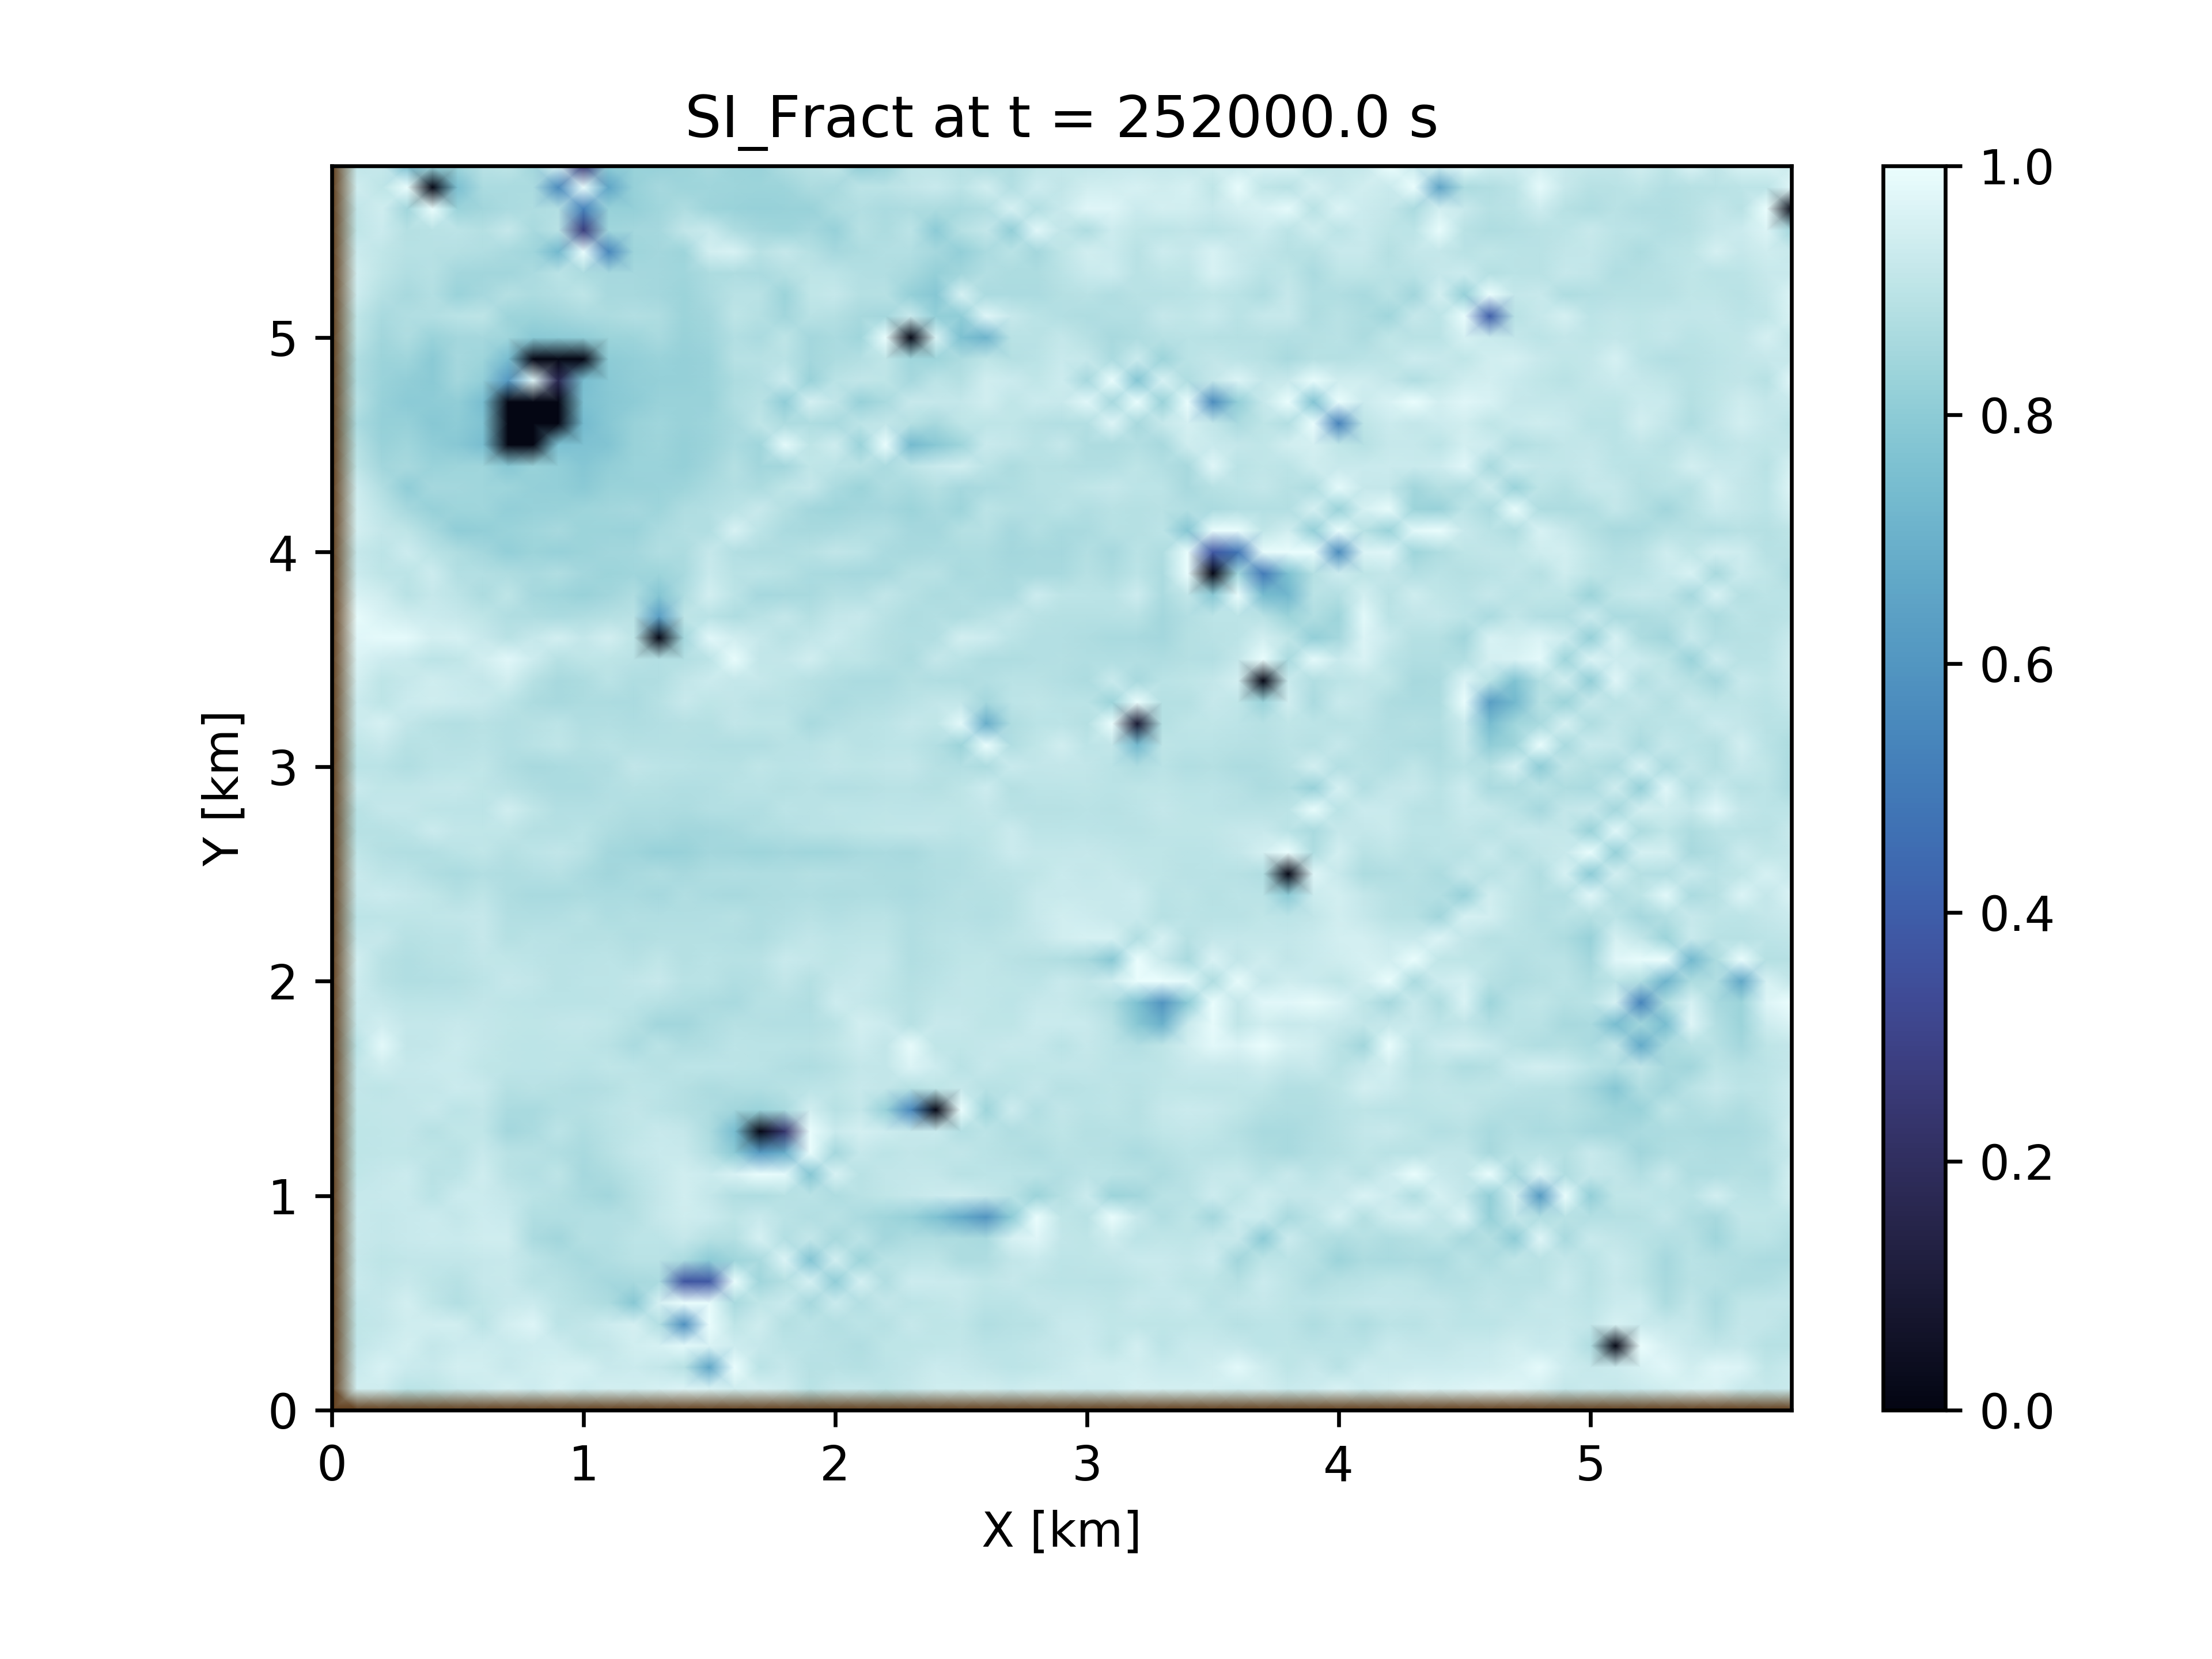
\includegraphics[width=\textwidth]{iceAdvect/advScheme-def-surface-ice-hd-0000025200.png}
	\end{subfigure}
 
	\begin{subfigure}{0.85\textwidth}
		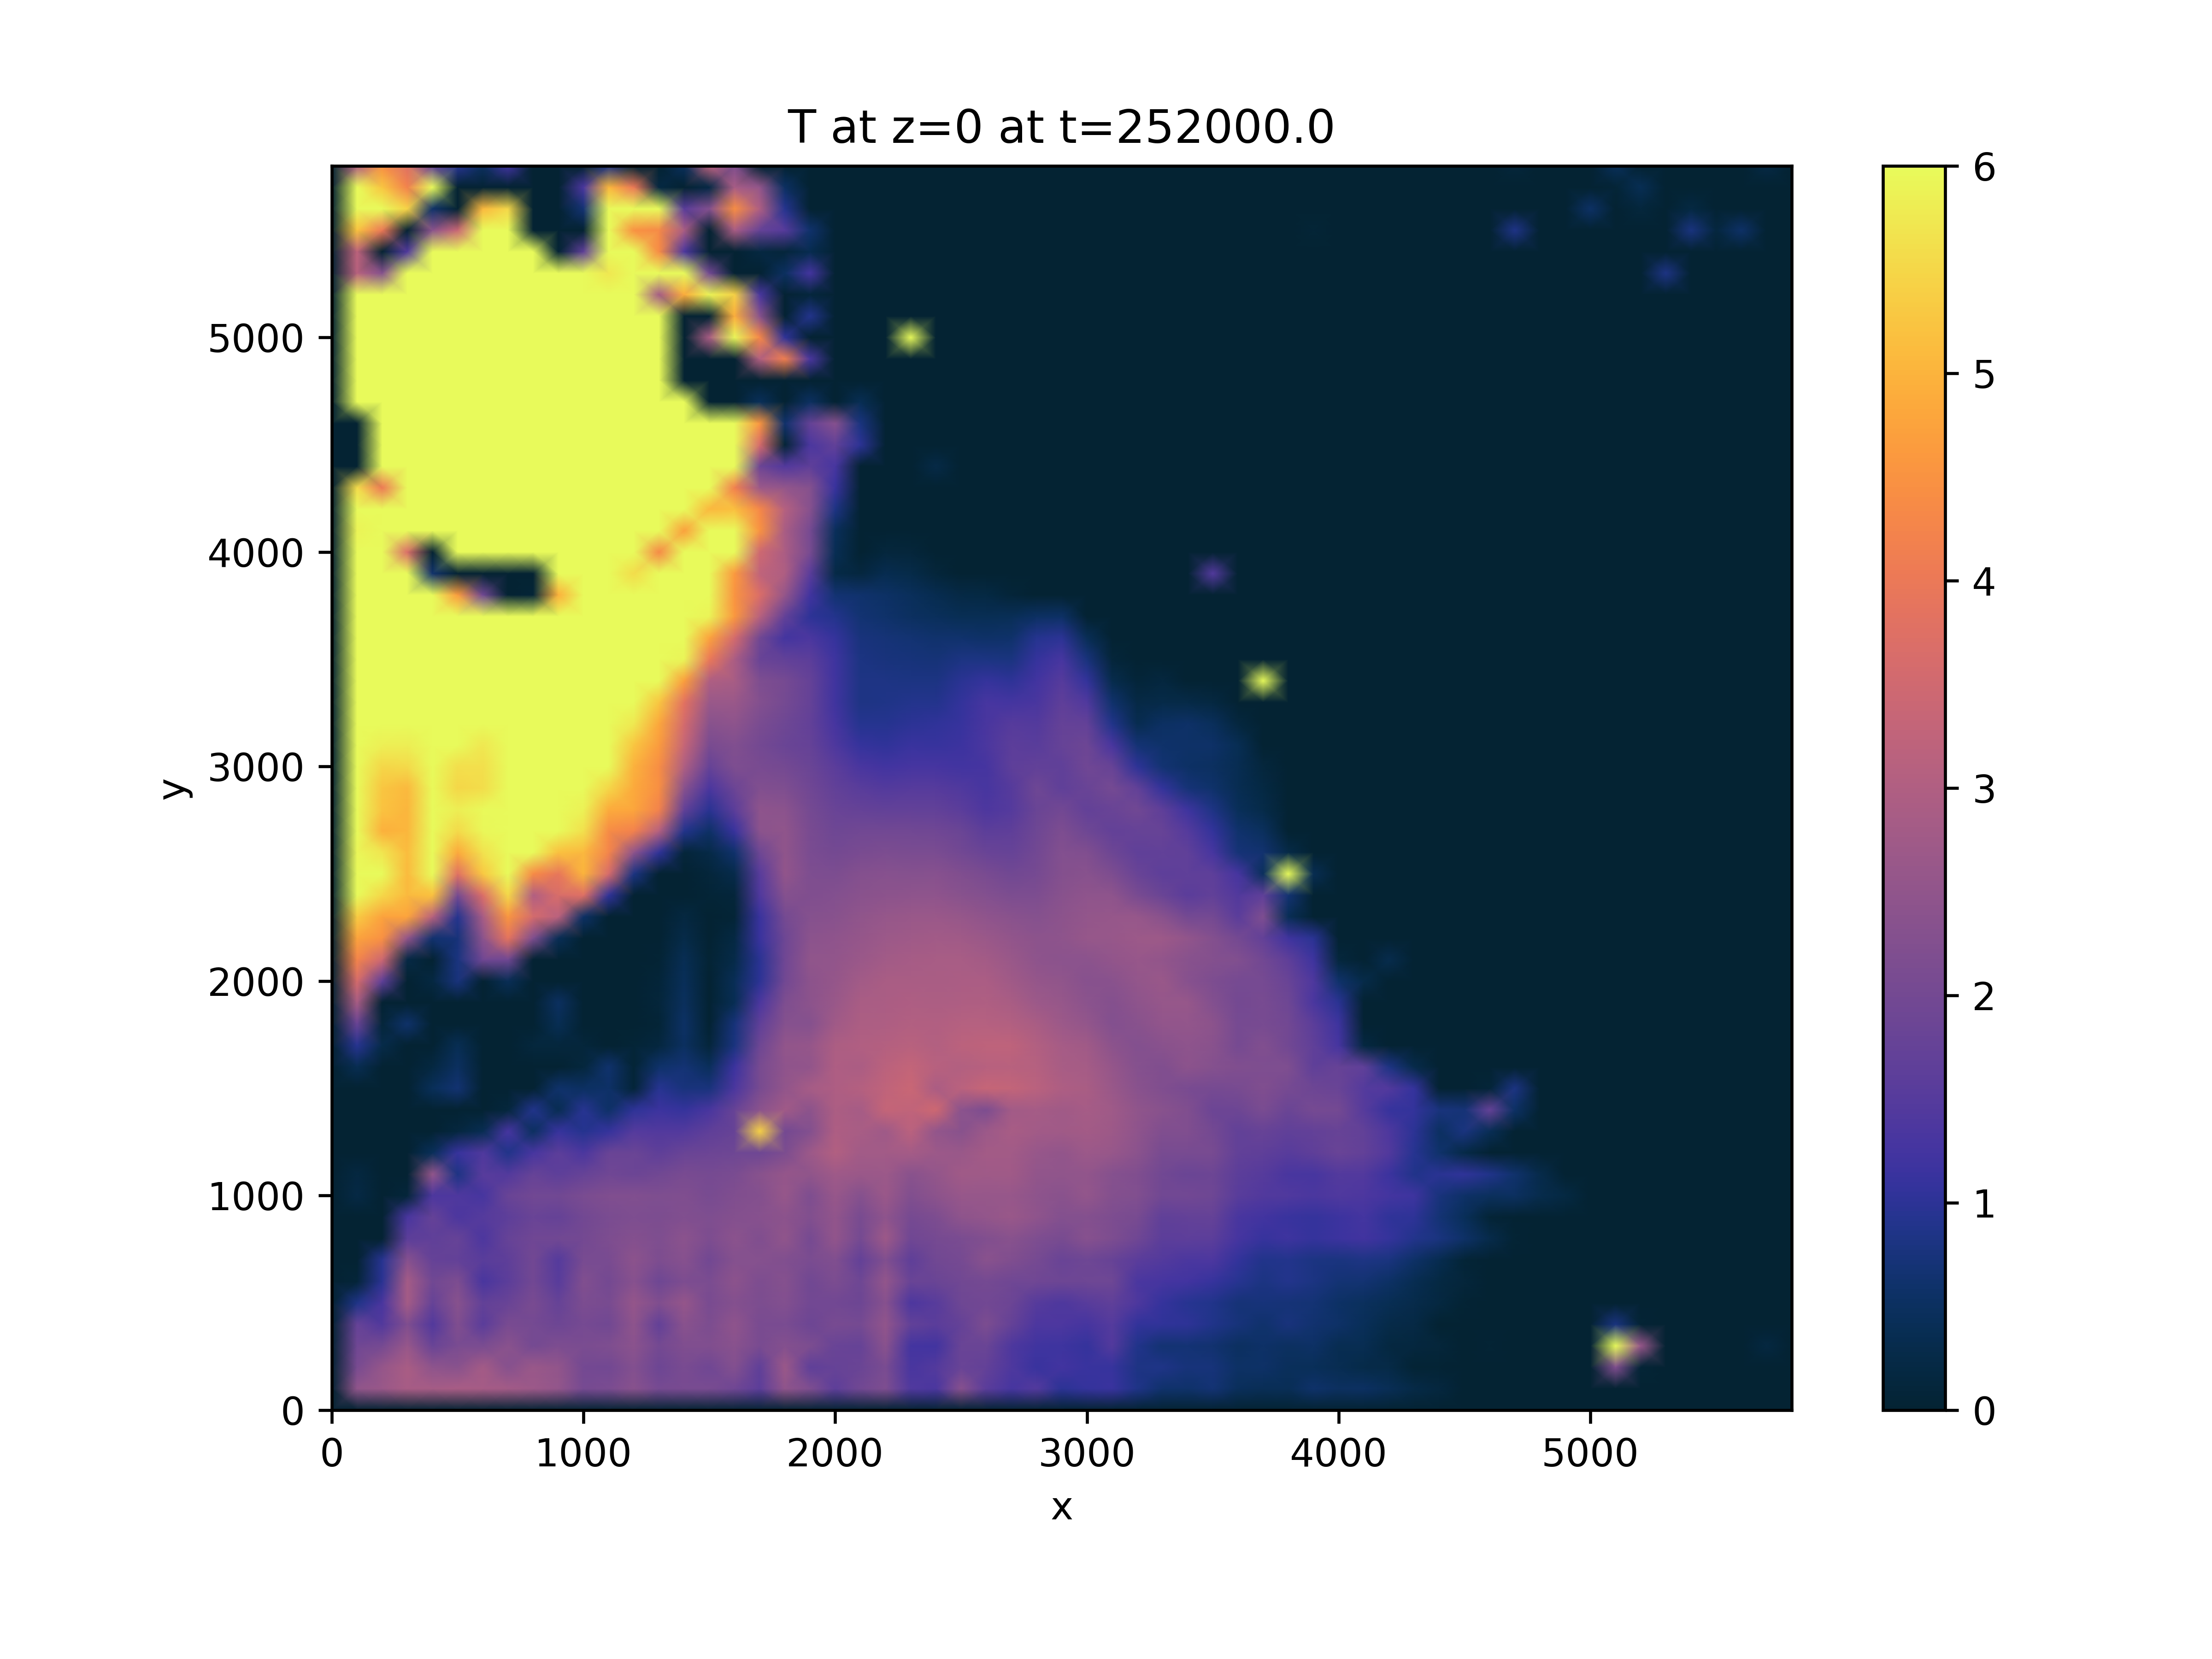
\includegraphics[width=\textwidth]{iceAdvect/advScheme-def-surface-T-hd-0000025200.png}
	\end{subfigure}
\caption{Case 1: Ice area fraction and temperature fields with advection scheme 2 (second order centered difference scheme). Note surface temperature much above freezing where ice has newly formed.}
\label{fig:advScheme2}
\end{figure}

\begin{figure}[h!]
\centering
	\begin{subfigure}{0.85\textwidth}
		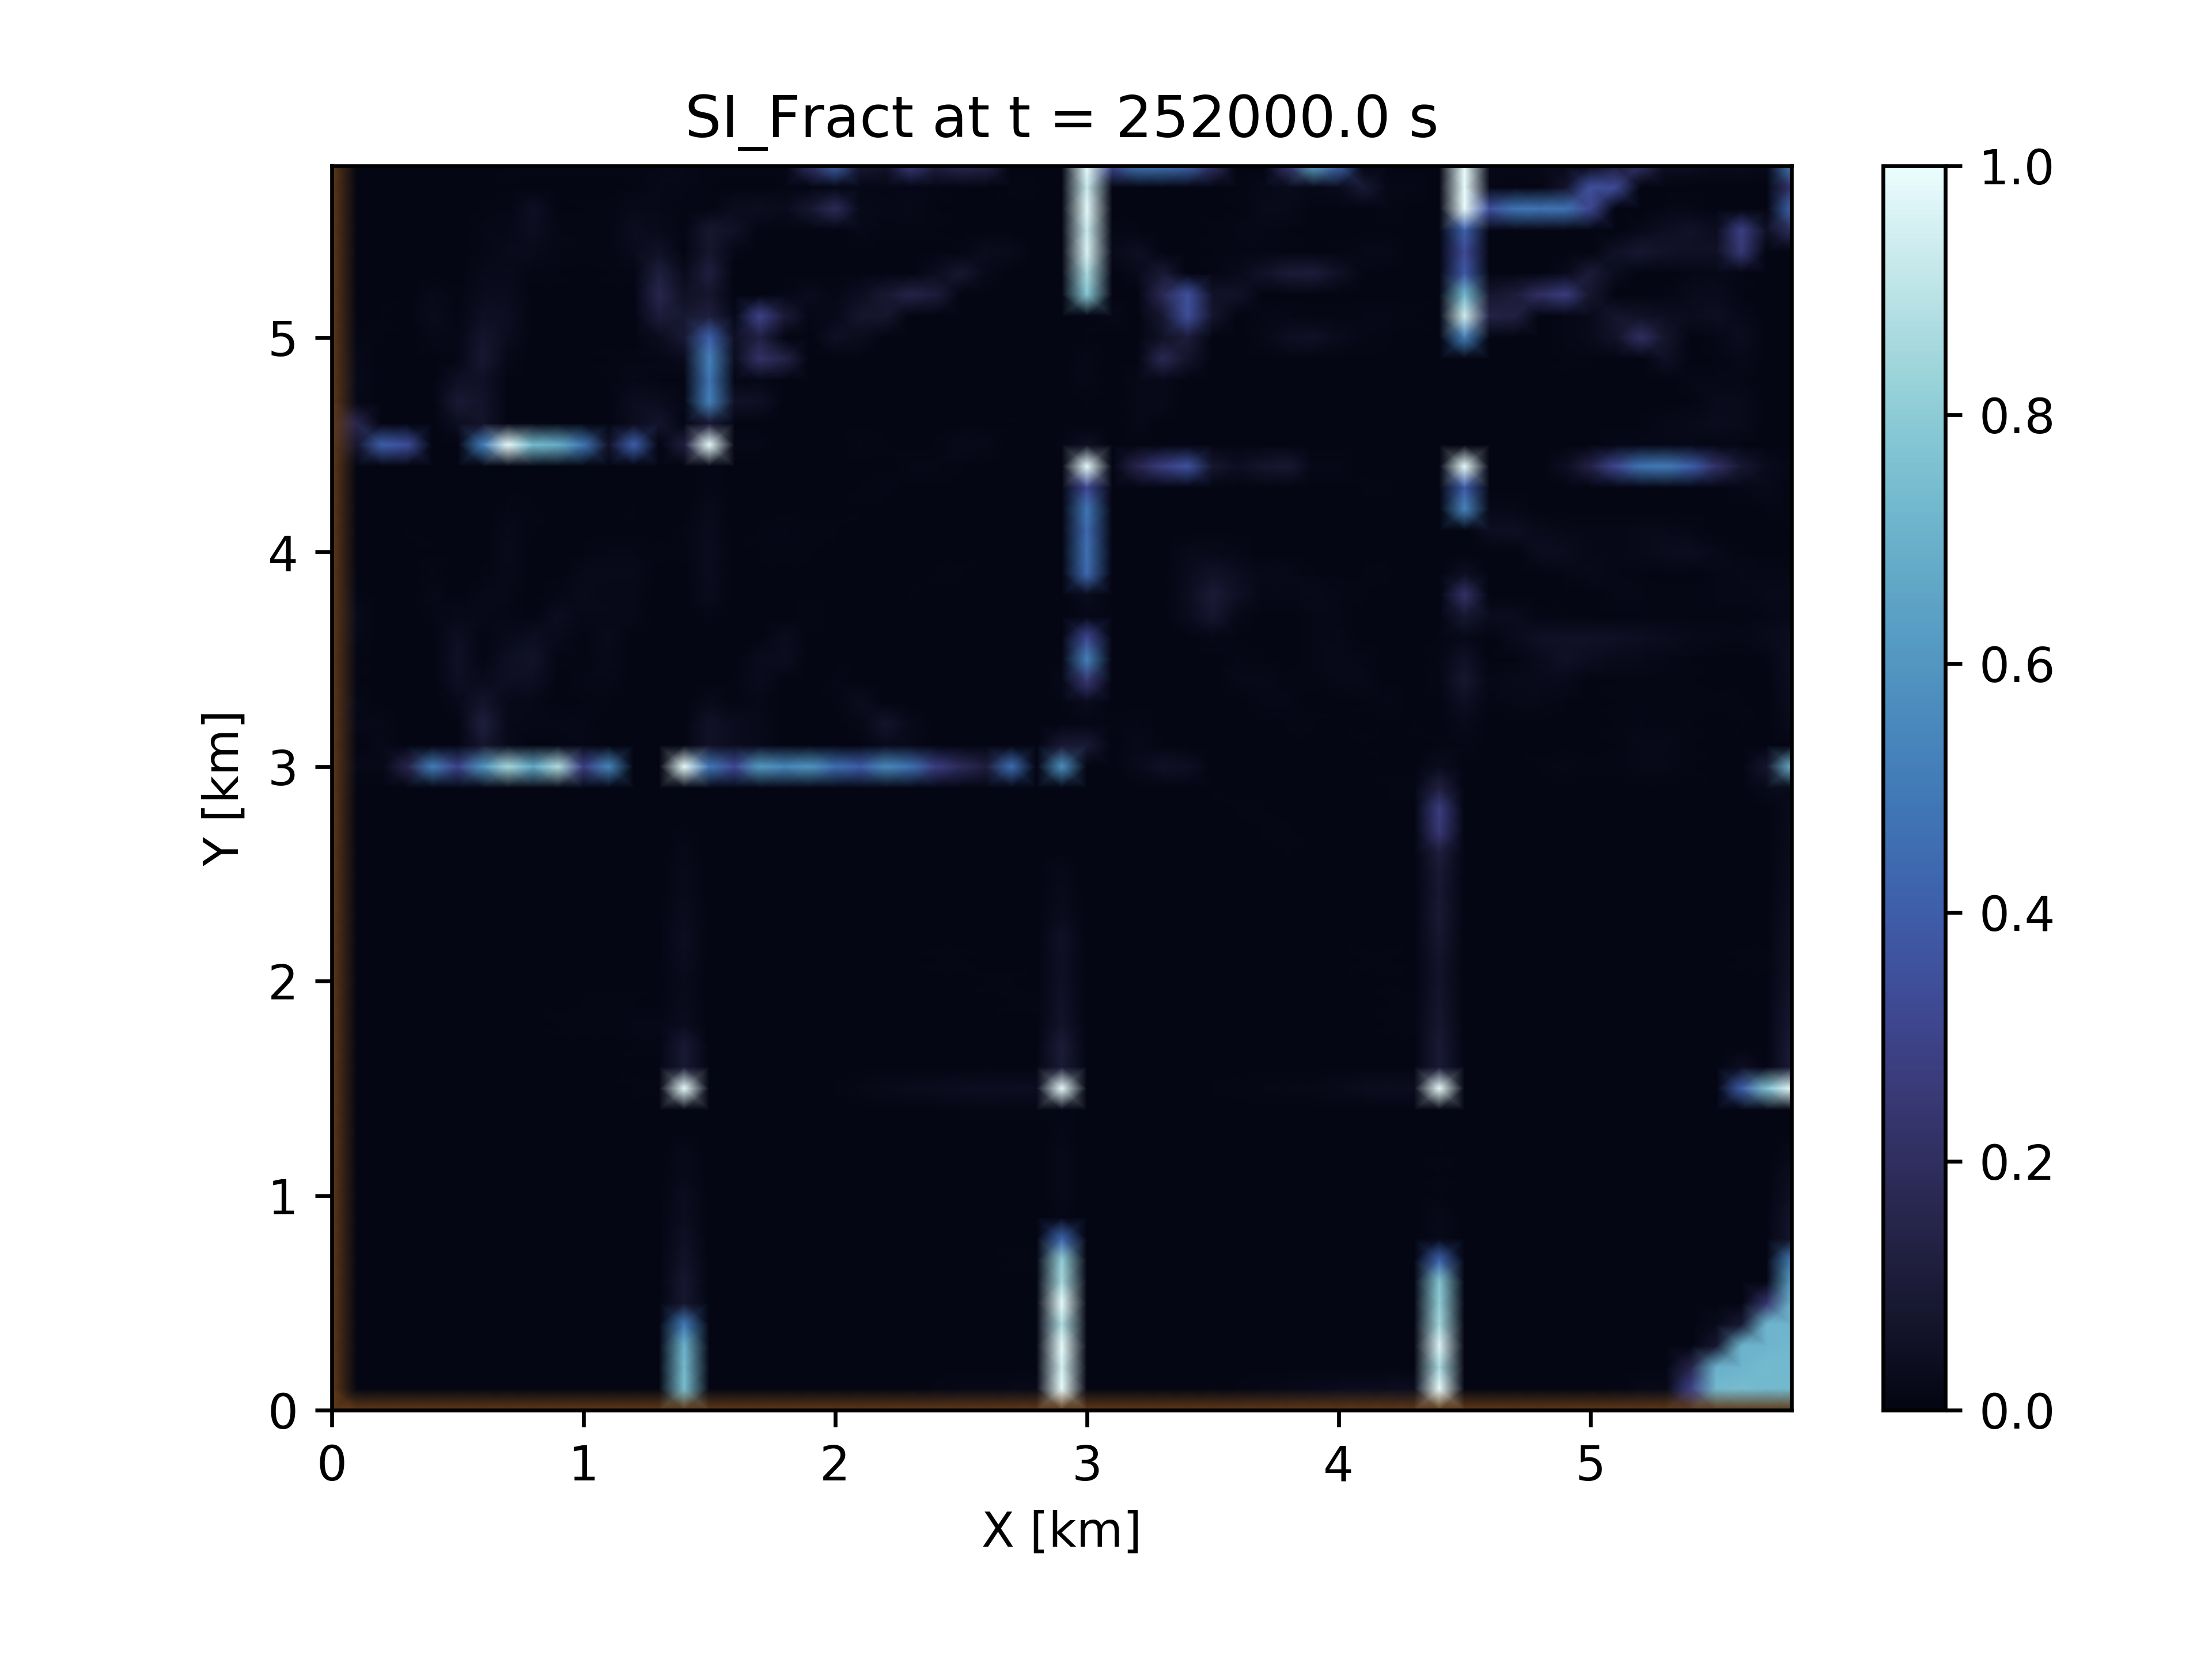
\includegraphics[width=\textwidth]{iceAdvect/advScheme-07-surface-ice-hd-0000025200.png}
	\end{subfigure}
 
	\begin{subfigure}{0.85\textwidth}
		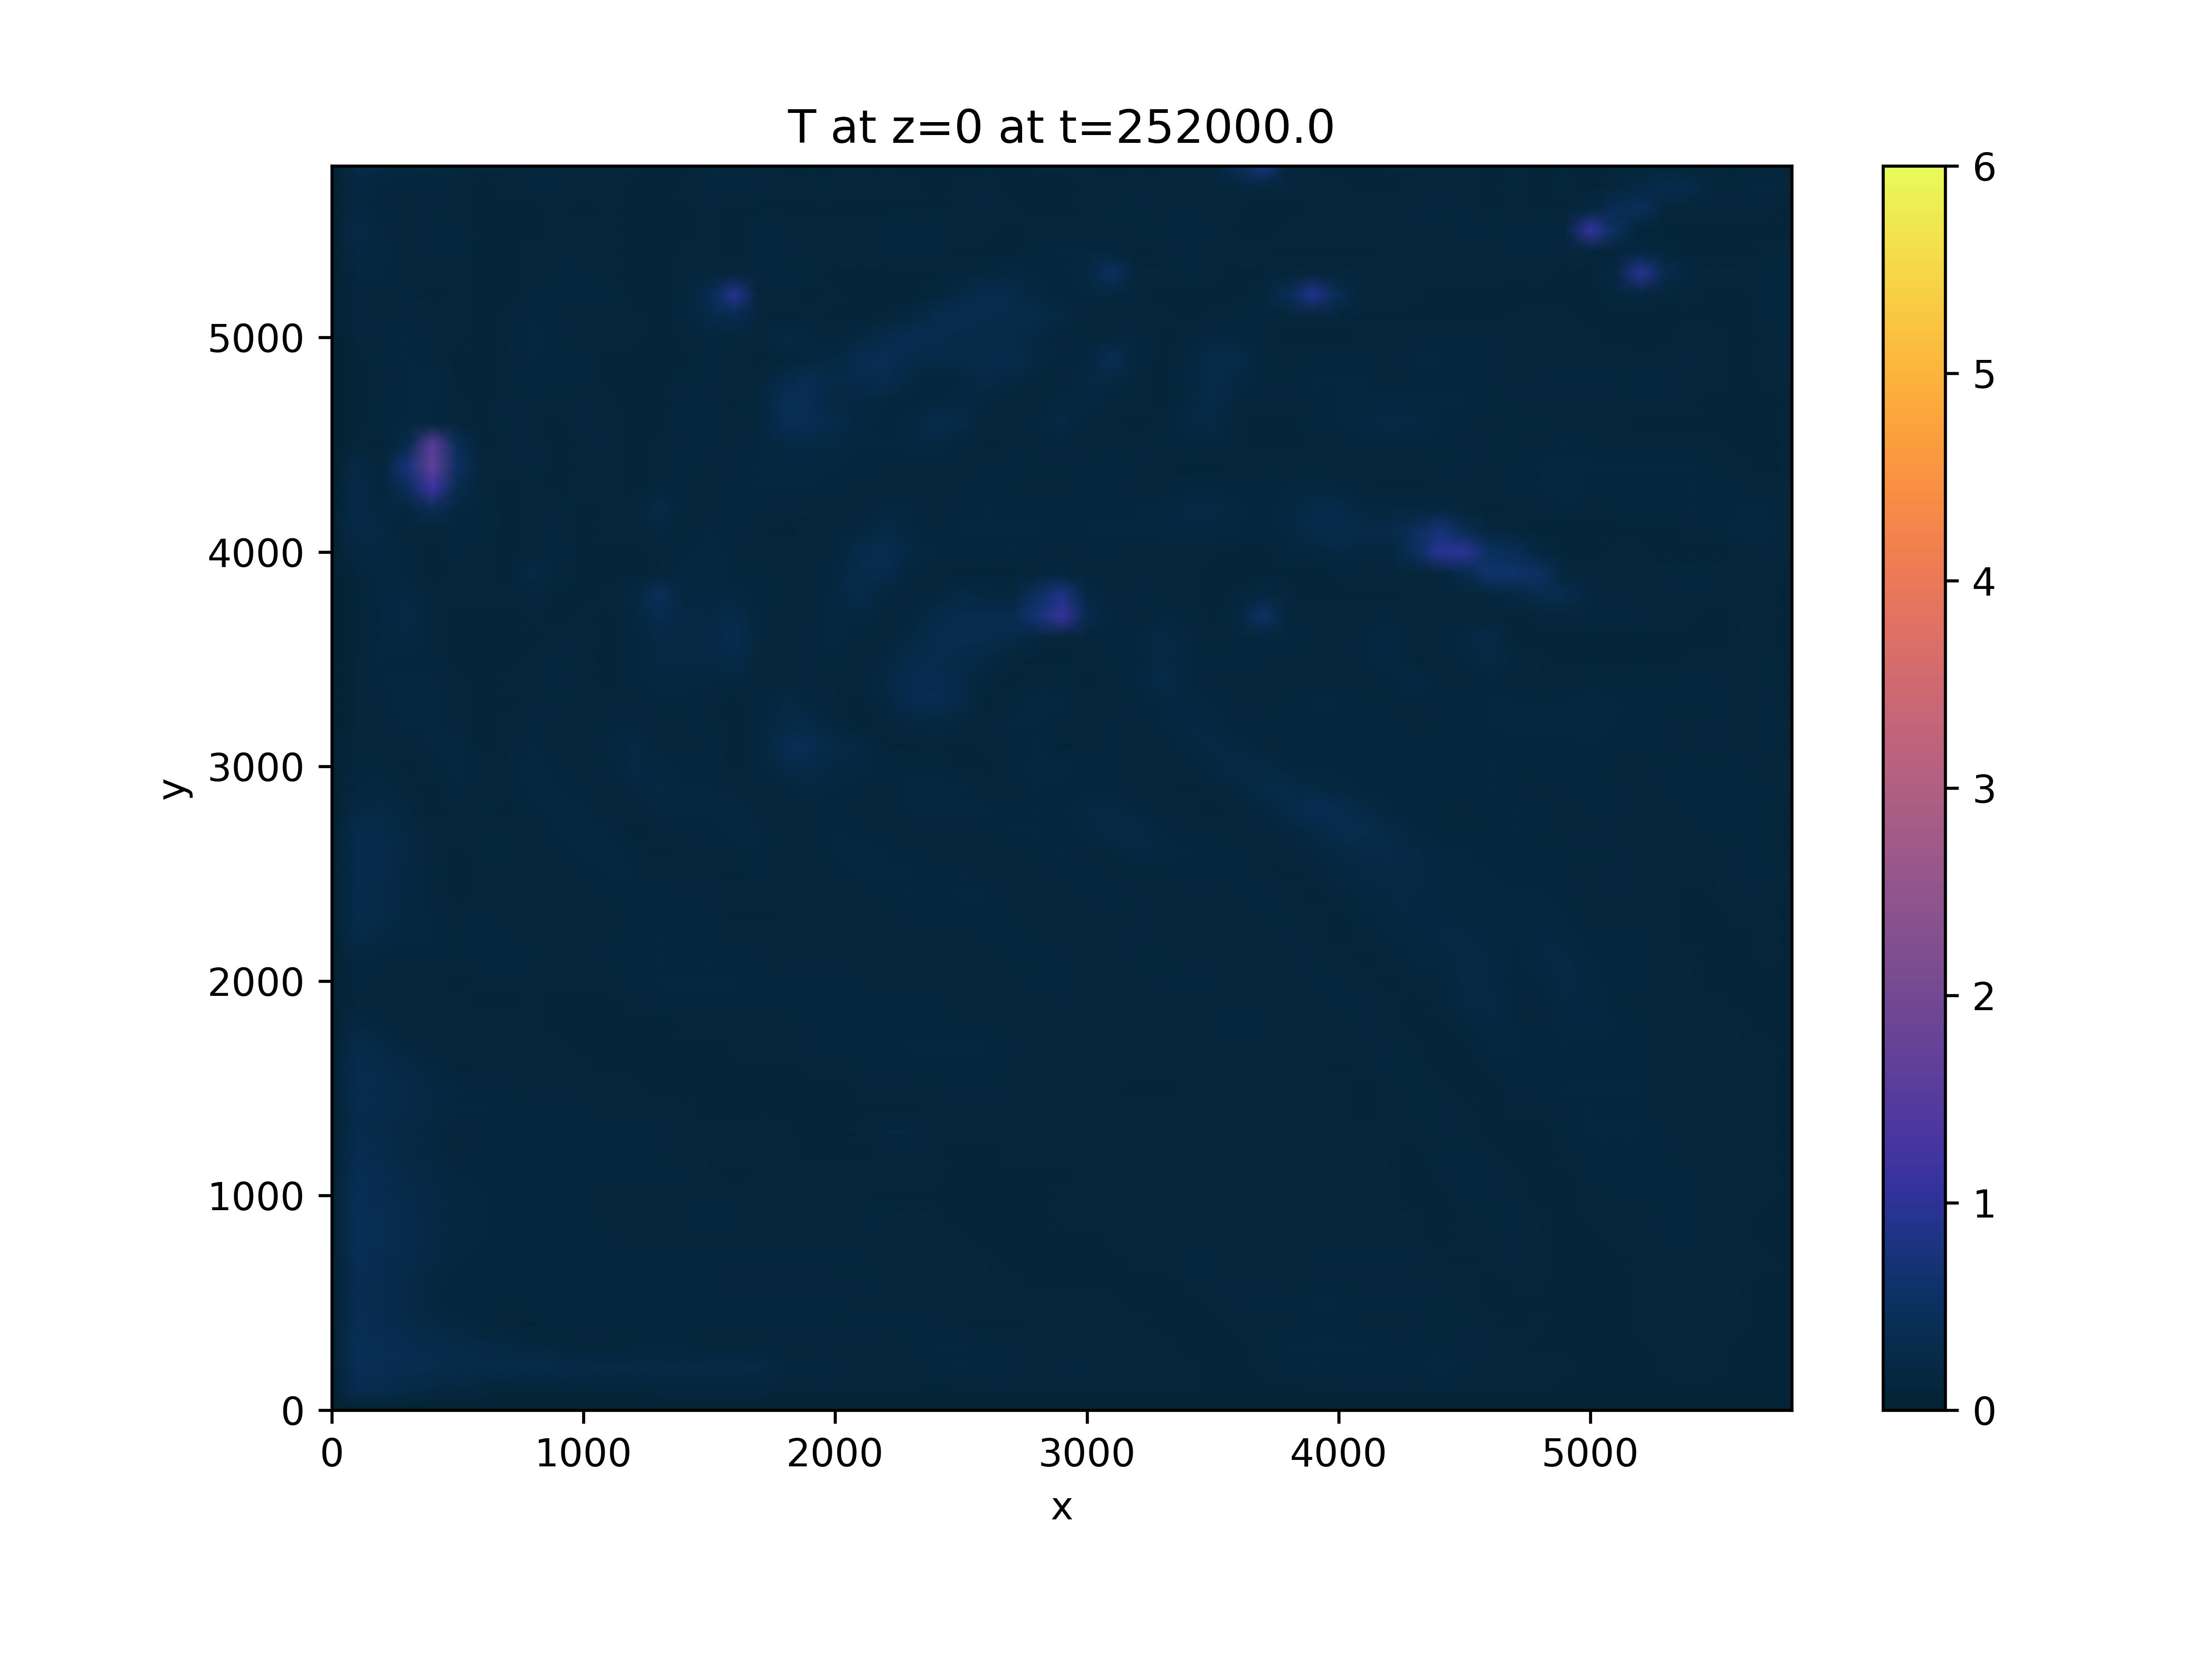
\includegraphics[width=\textwidth]{iceAdvect/advScheme-07-surface-T-hd-0000025200.png}
	\end{subfigure}
\caption{Case 1: Ice area fraction and temperature fields for advection sceheme 7. The obvious gridding pattern comes from the wrong overlap extent in X and Y.}
\label{fig:advScheme7}
\end{figure}

\clearpage

\begin{figure}[h!]
\centering
\begin{subfigure}{0.45\linewidth}
	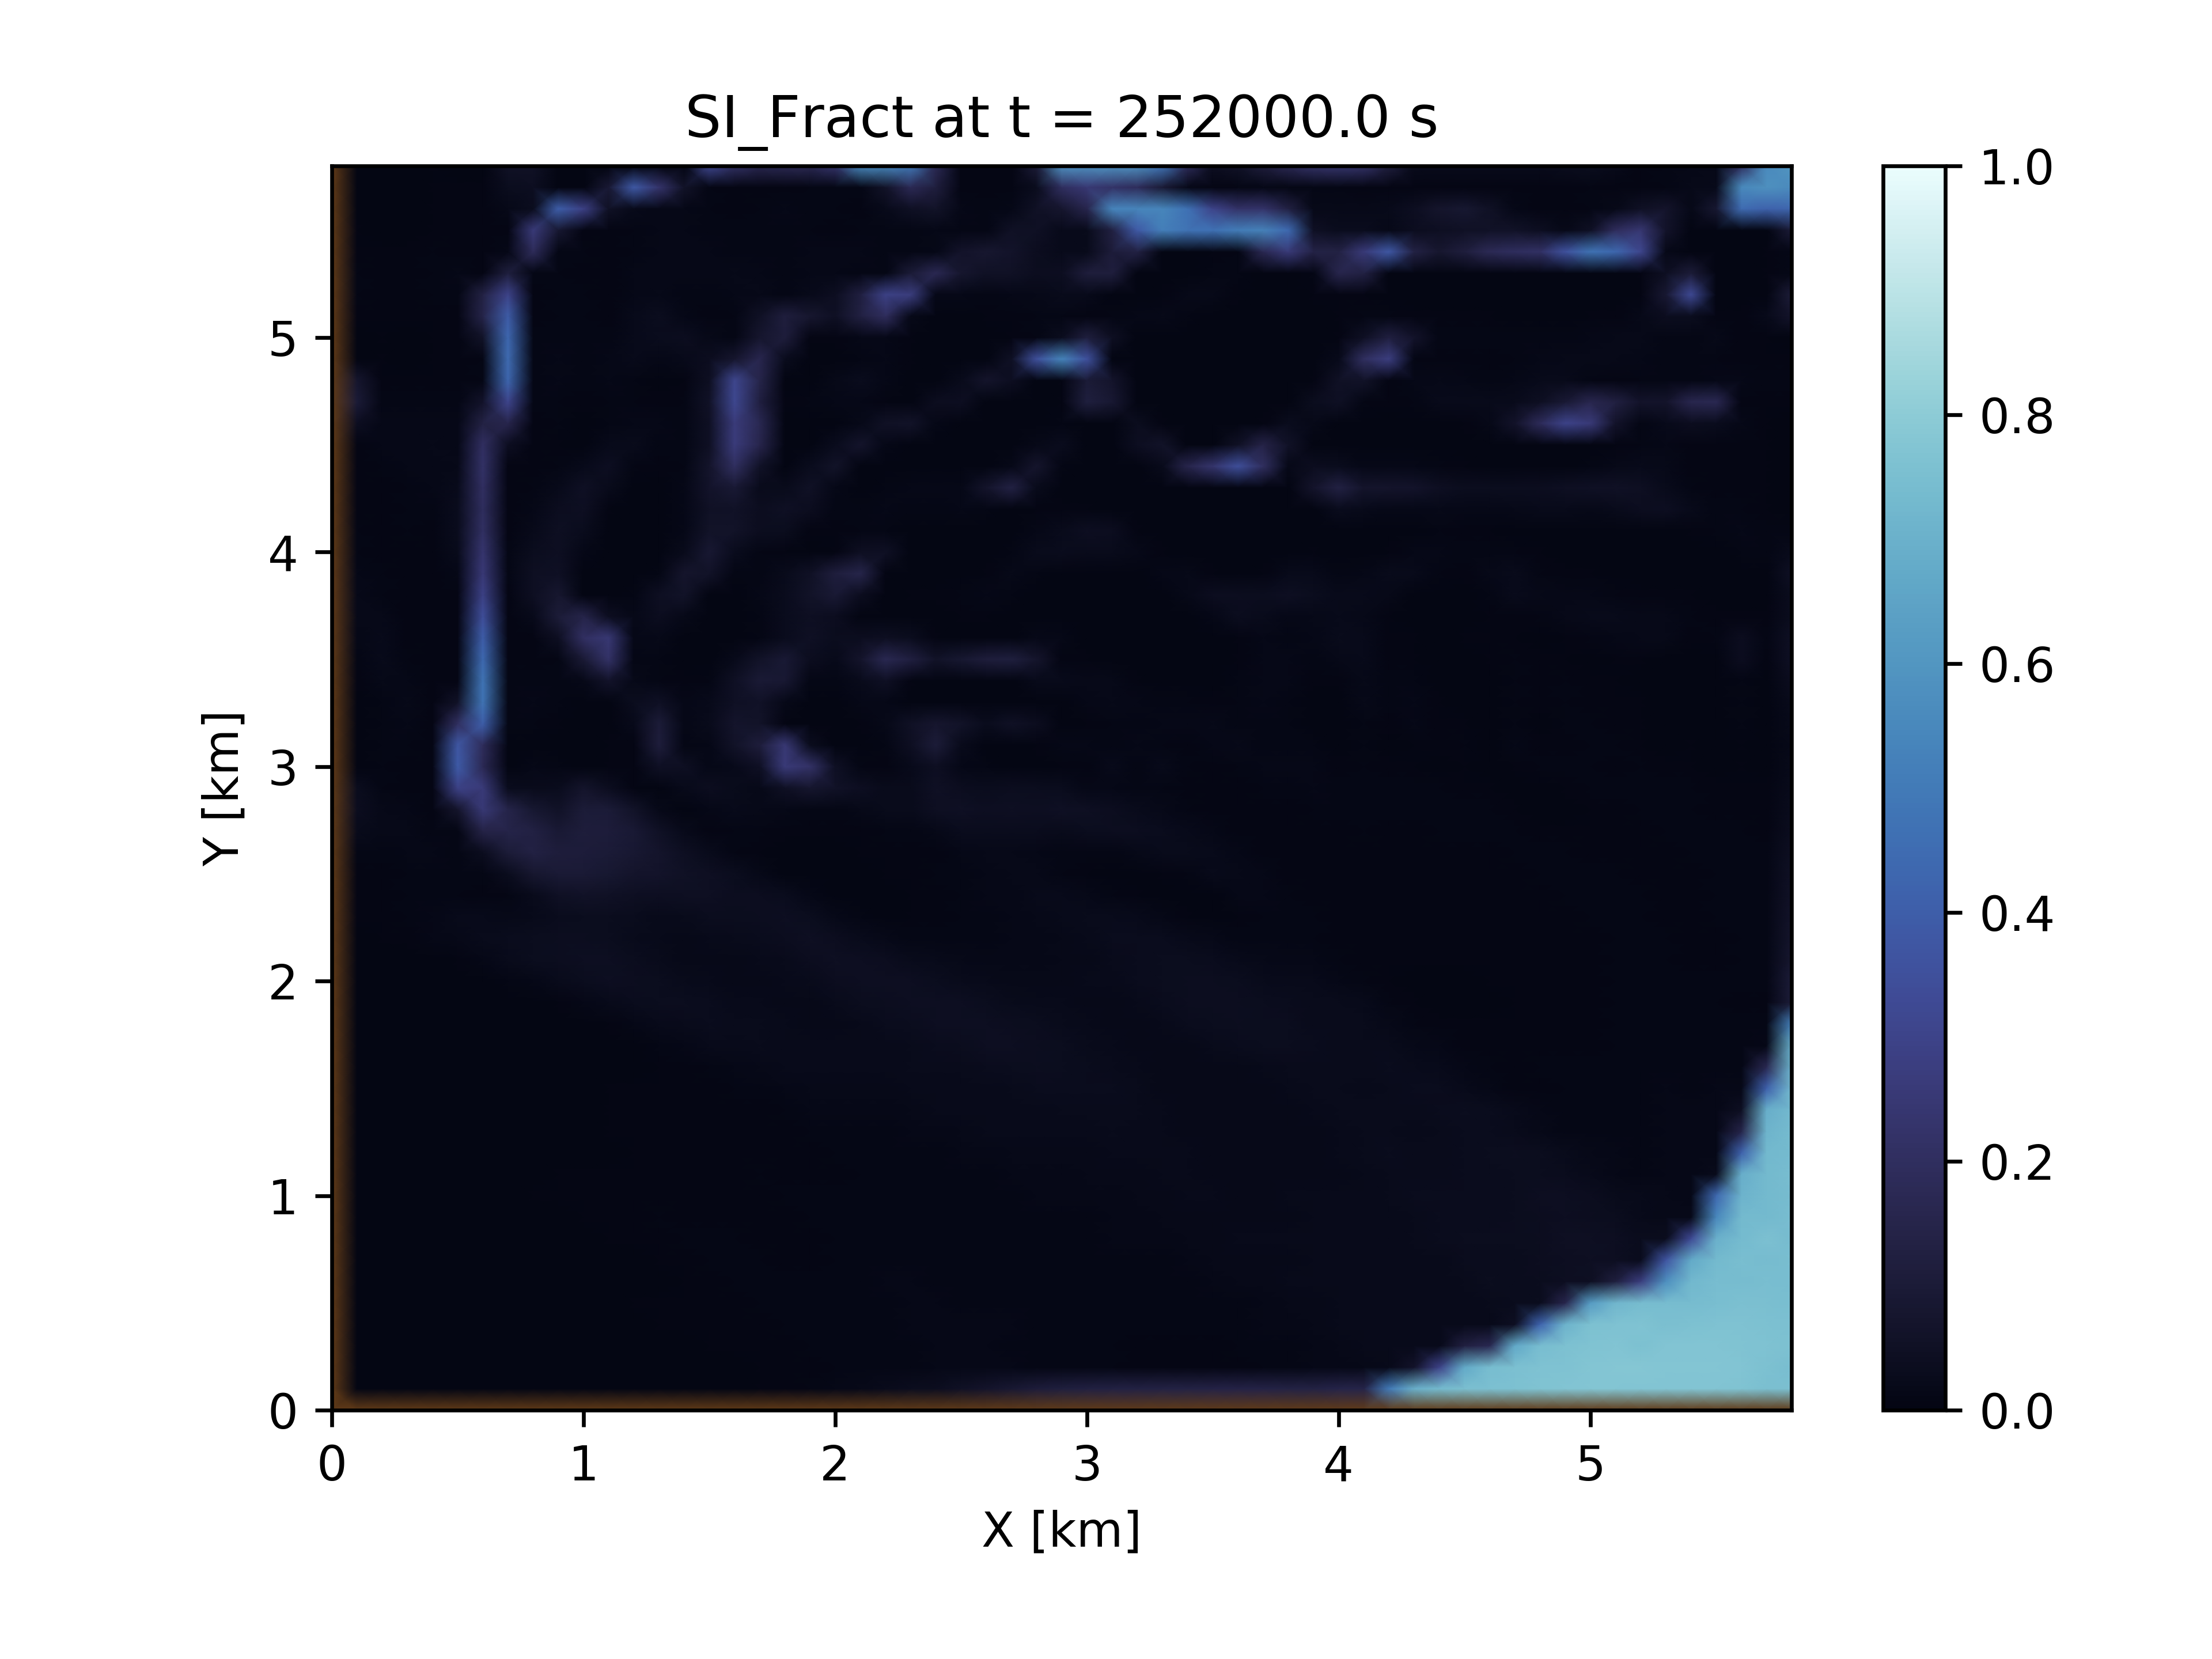
\includegraphics[width=\linewidth]{iceAdvect/advScheme-33-surface-ice-hd-0000025200.png}
\end{subfigure}
\begin{subfigure}{0.45\linewidth}
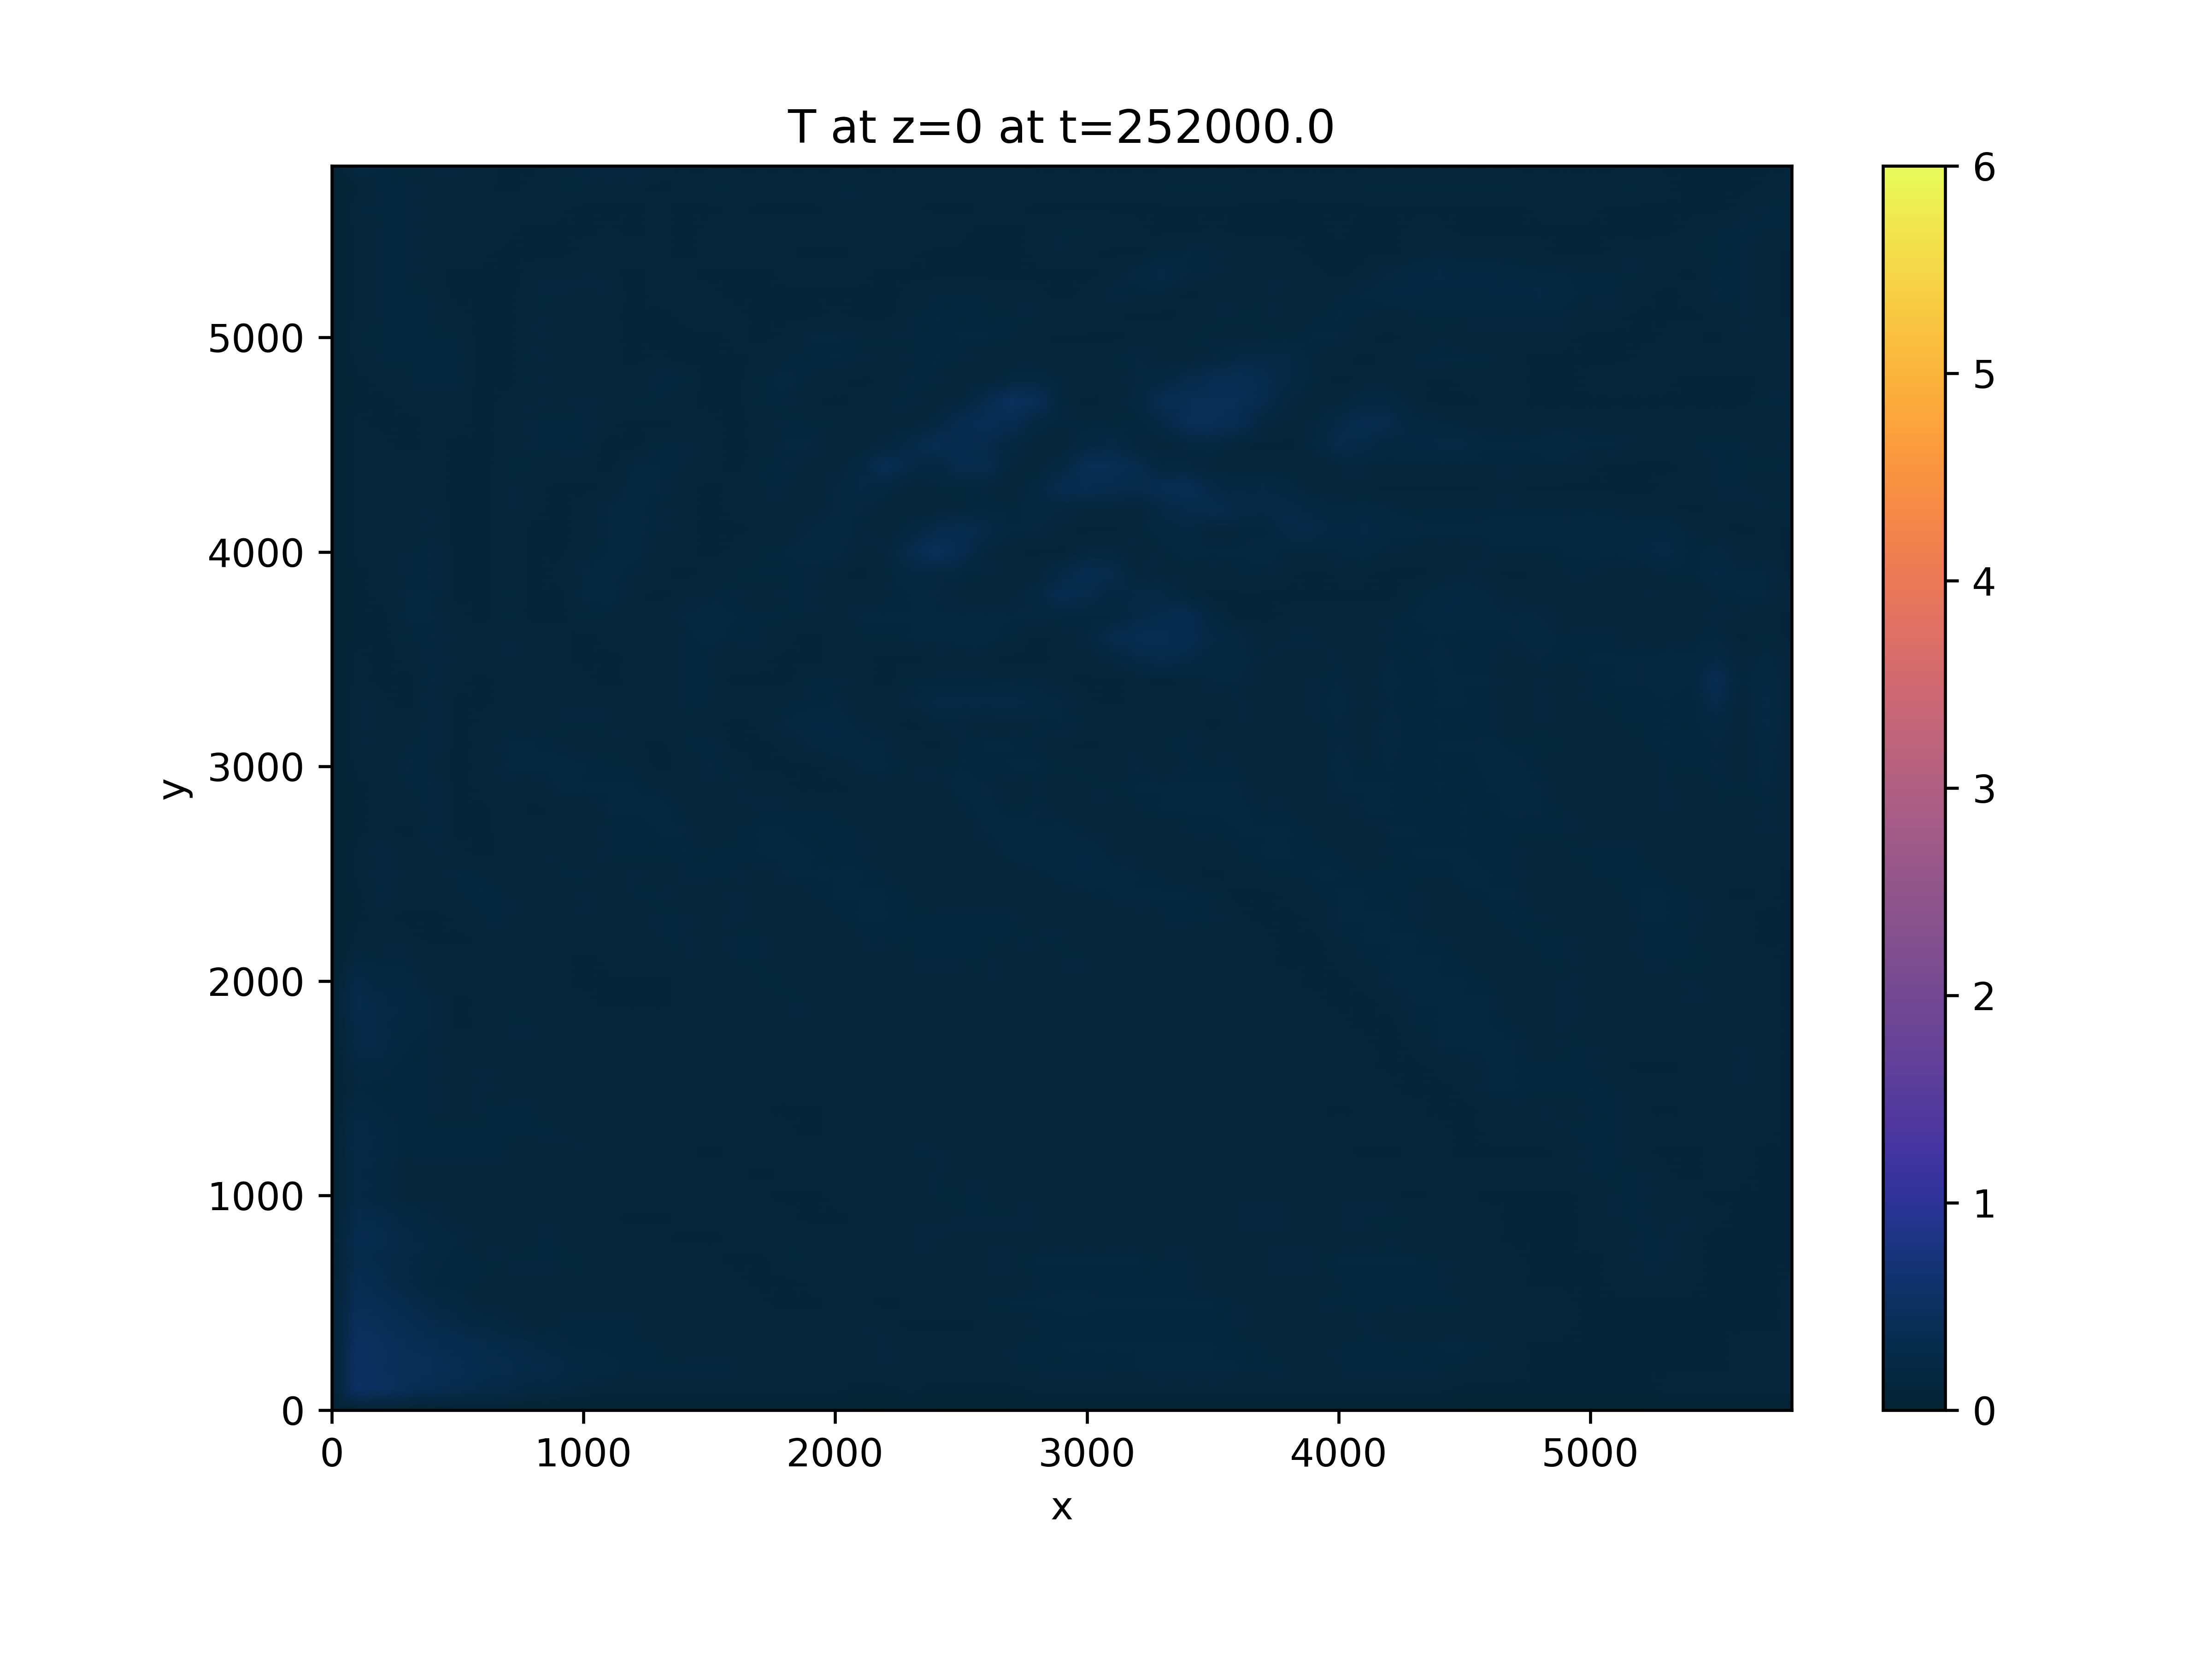
\includegraphics[width=\linewidth]{iceAdvect/advScheme-33-surface-T-hd-0000025200.png}
\end{subfigure}

\begin{subfigure}{0.45\linewidth}
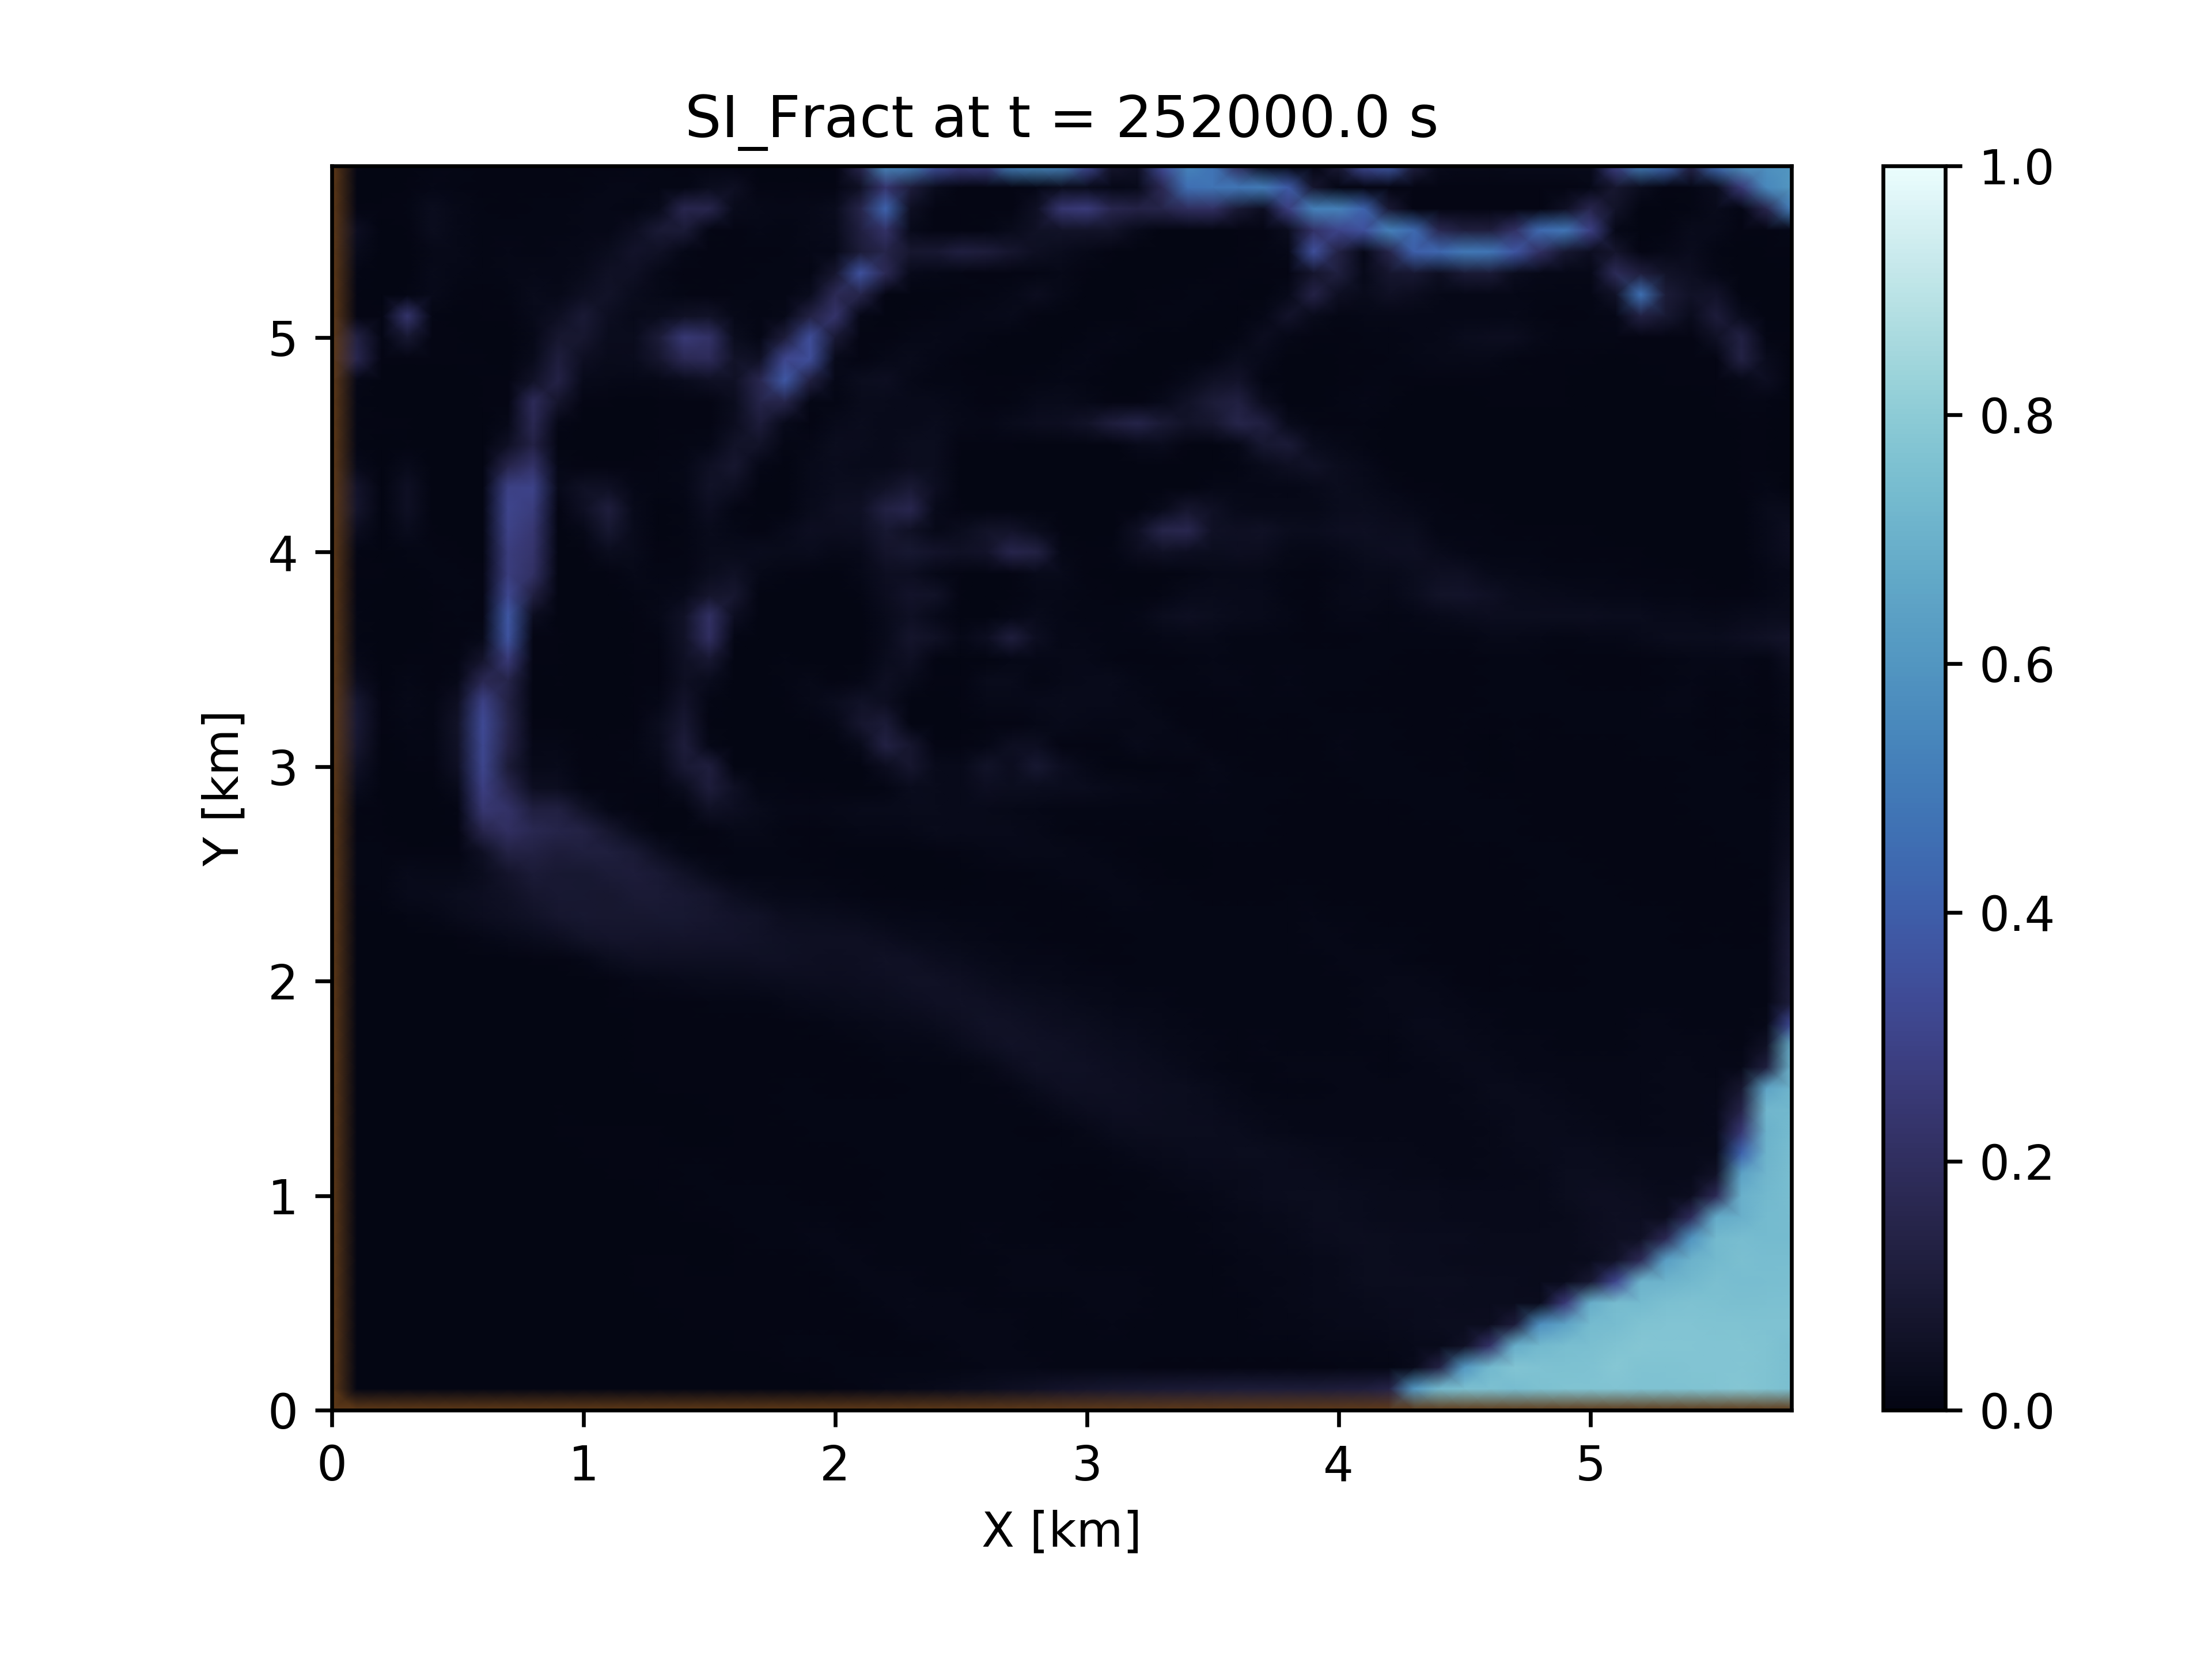
\includegraphics[width=\linewidth]{iceAdvect/advScheme-77-surface-ice-hd-0000025200.png}
\end{subfigure}
\begin{subfigure}{0.45\linewidth}
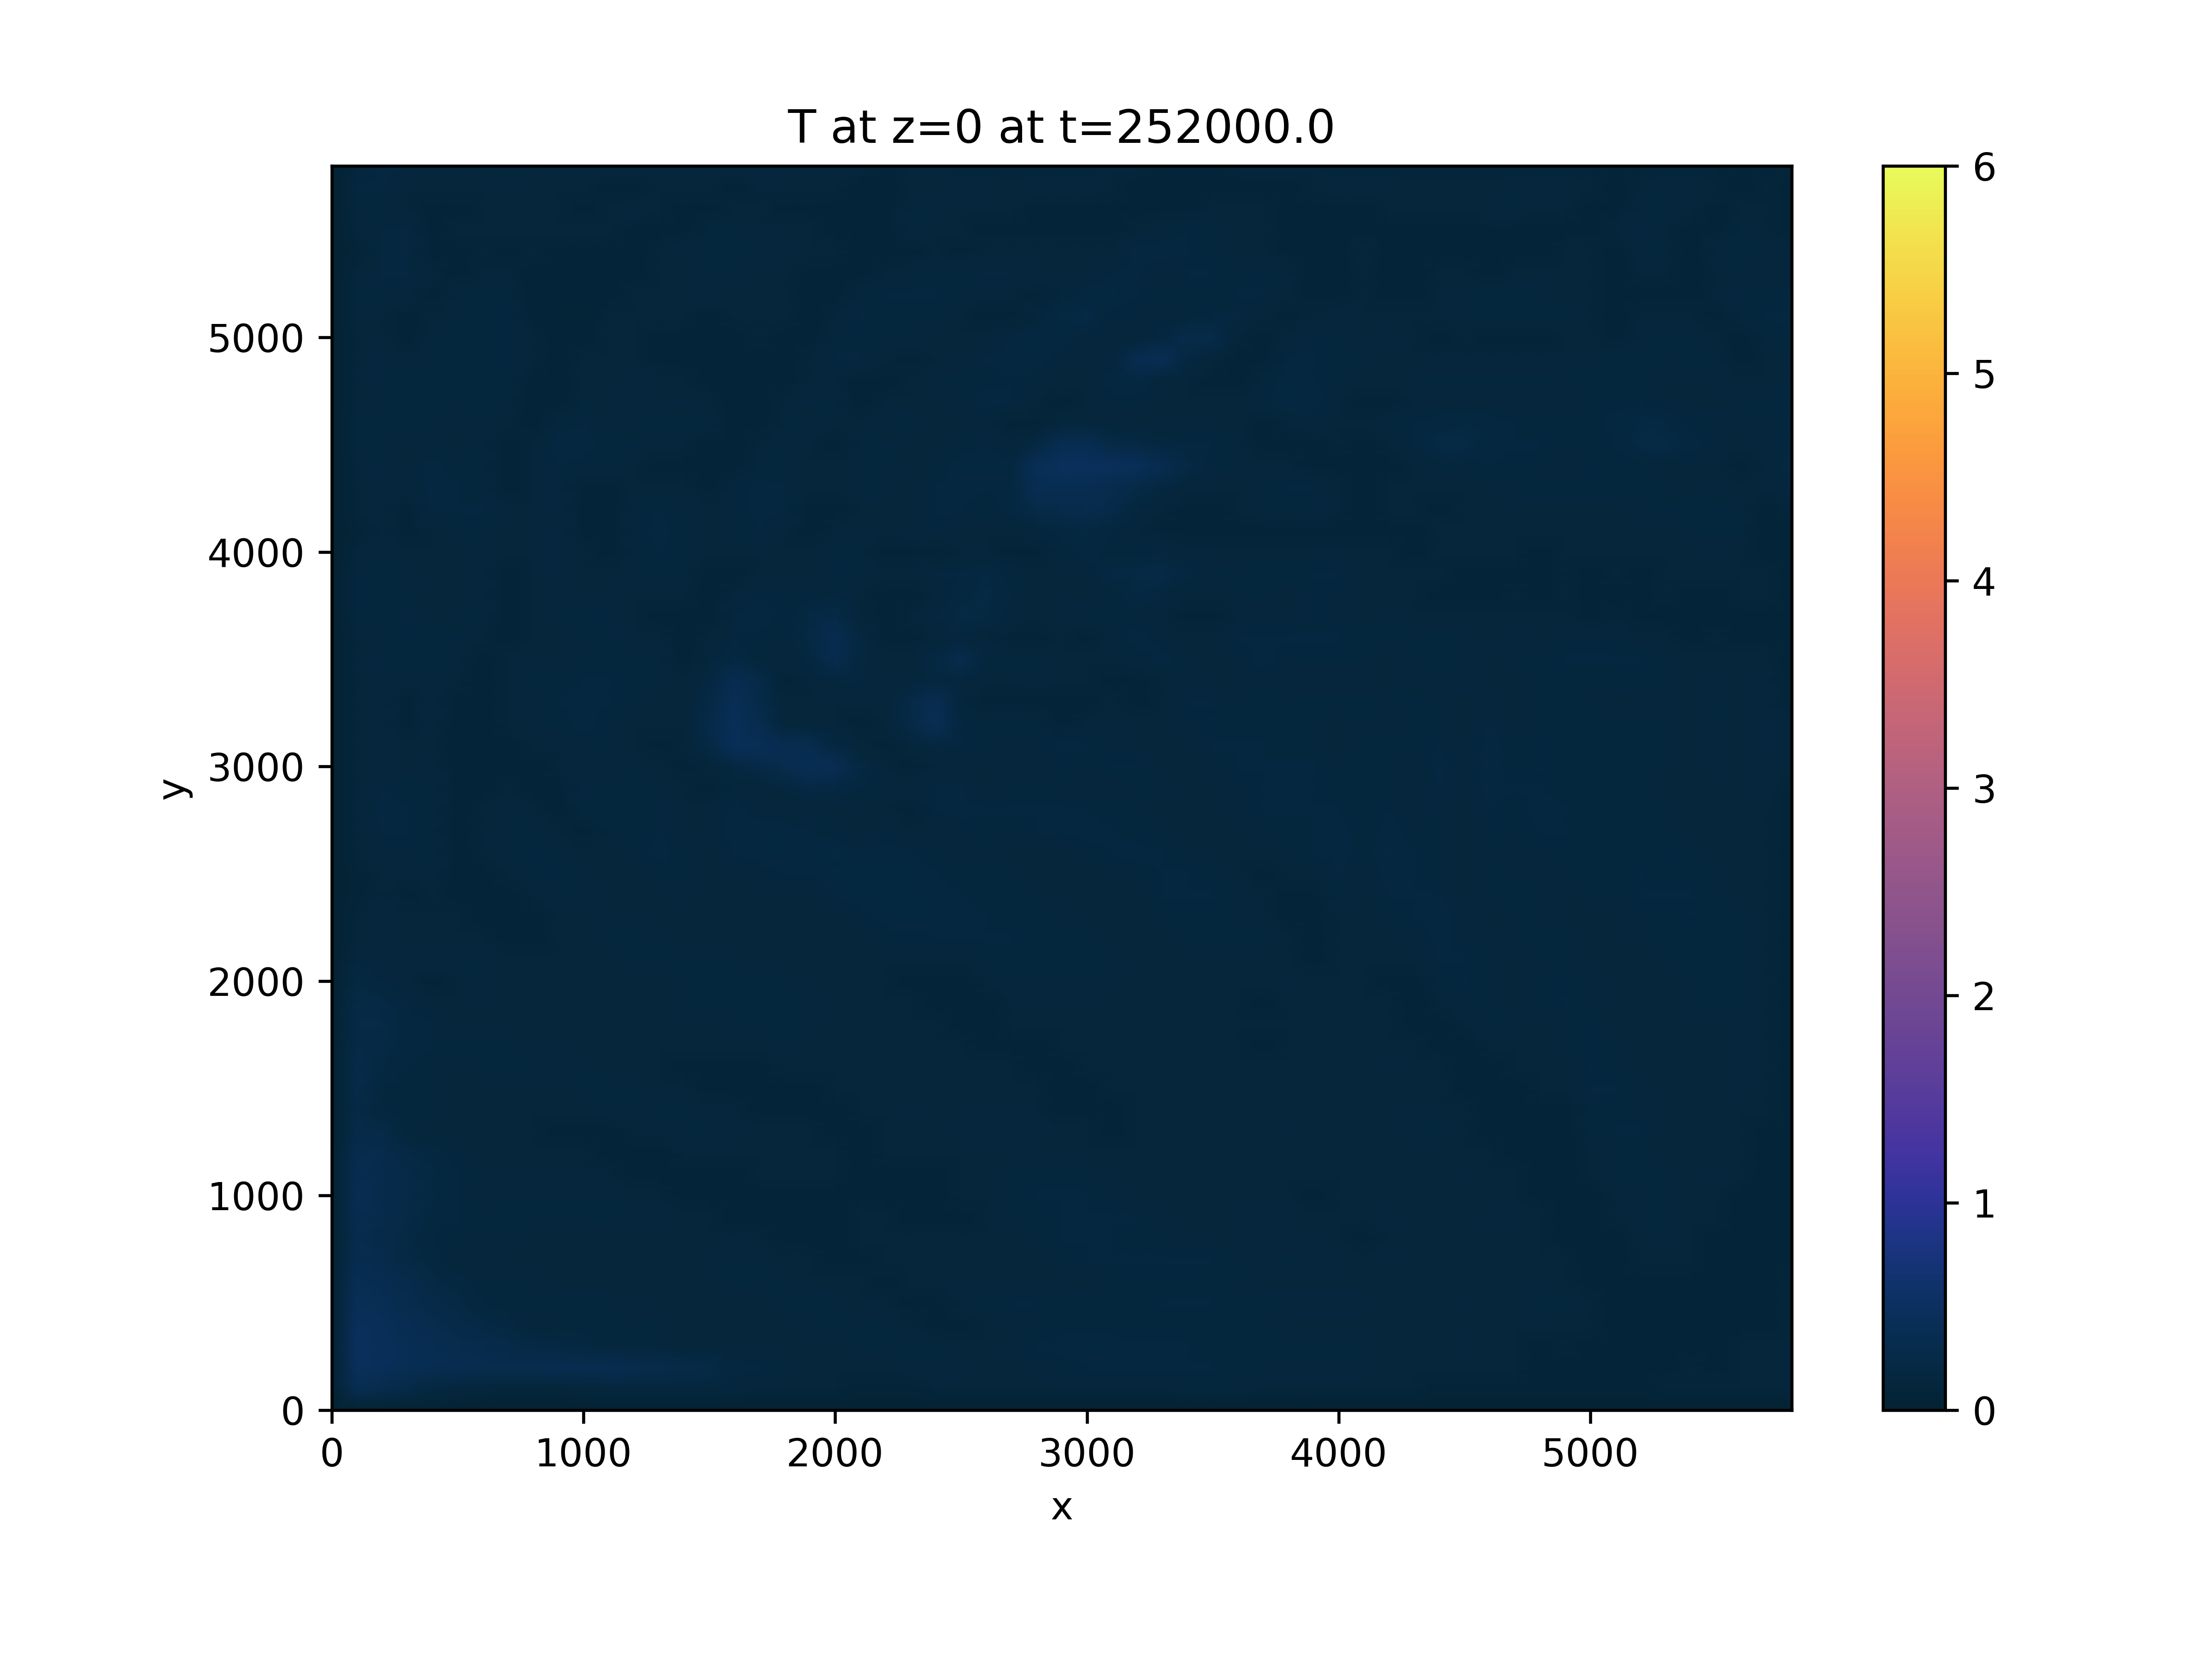
\includegraphics[width=\linewidth]{iceAdvect/advScheme-77-surface-T-hd-0000025200.png}
\end{subfigure}

\caption{Case 1: Ice area fraction and temperature fields for advection scheme 33 (top row) and 77 (bottom row). These agree qualitatively very well, and agree with physical intuition. }
\label{fig:advSchemes}
\end{figure}
The difference between the top and bottom of each panel in figure \ref{fig:advSchemes} is due to the wind. Ice forms in the top half where the water is calmer (because there is no wind there), gets pushed by the surface currents, and then in the bottom half is pushed quickly by the wind. It collects in the bottom right corner.


\subsubsection{What was learned}
From this simulation, we learned and see the following points
\begin{itemize}
\item{With a good advection scheme (33 or 77, high dimensional with flux limiter) the ice is advected physically by the wind and surface currents.}
\item{The water was cooled by the cold air}
\item{Ice melted at first because of the warm water. Ice forms later on when the surface temperature is at or below 0 (assuming we have a good advection scheme).}
\item{The Linear equation of state is a poor choice. Looking at temperature cross-sections the cold water falls to the bottom, and water closer to $\SI{4}{\celsius}$ rises to the top. This is opposite from what should happen. A more accurate EOS would form ice faster since cold water would stay at the top.}
\end{itemize}

\subsection{Case 2: Ice melting}
We wanted to design a scenario which would isolate how the model melts ice. The lake is initialized with constant ice cover, with warm air and moderate downward solar radiation (see complete details in table \ref{table:iceMelt}. There are eastward winds in the south half of the lake. We expect the ice to melt and break up. In particular, we want to see:

\begin{itemize}
\item{Ice to melt until it starts to break up}
\item{The ice to start being moved around once it has space to move (once there is some open water)}
\item{Ice to completely melt, water to be heated by the radiation and air}
\end{itemize}

\begin{longtable}{  p{.30\textwidth}  p{.30\textwidth}  p{.4\textwidth}  }
\hline
\textbf{Paramter Name} & \textbf{Parameter Value} & \textbf{Comment} \\ \hline \hline
\verb|Nx| & 600 & 50 x 12 processors \\ \hline
\verb|Ny| & 600 & 50 x 12 processors \\ \hline
\verb|tempAdvScheme|	&	33	&	High order advection scheme \\ \hline
\verb|nonHydrostatic| & \verb|.FALSE.| & Use hydrostatic configuration \\ \hline
\verb|eosType|		&	JMD95z	&	Polynomial approximation to true equation of state. This EOS respects the max in density at $4^{\circ} \textrm{C}$\\ \hline
\verb|delX|			&	\verb|600*10.0|	&	6 km lake, 100 m resolution \\ \hline
\verb|delY|			&	\verb|600*10.0|	&	6 km lake, 100 m resolution \\ \hline
\verb|delZ|			&	\verb|100*0.1 |	&	10 m deep lake, 0.5 m resolution \\ \hline

\verb|uwind|		&	\begin{equation*} \begin{cases} 1.0 \text{ m/s} & y \leq 3 \text{km} \\ 0 \text{ m/s} & y > 3 \text{km}   \end{cases} \end{equation*} & \\ \hline
\verb|vwind| 	& 0	& \\ \hline
\verb|atemp| 	& $10^{\circ} \text{C}$		& Constant cold air temperature \\ \hline
\verb|aqh| 		& $0.01$		&	Specific humidity \\ \hline
\verb|swdown| 	& $300 \text{ W} \text{ m}^{-2}$	& Minimum shortwave downward radiation \\ \hline
\verb|lwdown| 	& $300 \text{ W} \text{ m}^{-2}$	& Minimum longwave downward radiation \\ \hline

\verb|SEAICEuseDYNAMICS| & \verb|.TRUE.| & Allow SEAICE dynamics \\ \hline
\verb|SEAICE_area_reg|   & \verb|1.0E-5| & Ice fraction less than this will be treated as zero ice for next time step \\ \hline
\verb|SEAICE_hice_reg|   & \verb|1.0E-5| & Height cutoff \\ \hline
\verb|SEAICEadvHEFF|     & \verb|.TRUE.| & Advect effective height \\ \hline
\verb|SEAICEadvAREA|     & \verb|.TRUE.| & Advect seaice area fraction \\ \hline
\verb|SEAICEadvScheme|   & $33$			& Advection scheme 33: Flux limited direct space and time advection scheme \\ \hline

Temperature & \begin{equation*} \begin{cases} 0^{\circ} \text{C} & z = 0 \text{ m} \\ 4 ^{\circ} \text{C} & z = -10 \text{ m}   \end{cases} \end{equation*} & Temperature stratified lake \\ \hline
Initial SEAICE area fraction   & $0.9$ & Constant ice covered fraction \\ \hline
Initial SEAICE thickness    & $0.1$ & Constant ice thickness \\ \hline

\caption{Parameter values for case 2: ice melt}
\label{table:iceMelt}
\end{longtable}
The model was run with these parameters, as well as:
\begin{itemize}
\item{Change \verb|nonHydrostatic| to \verb|.TRUE.| to test sensitivity to hydrostatic/non-hydrostatic configuration}
\item{Double the number of grid points in X and Y to test resolution sensitivity}
\item{Set surface winds to 0 to test effect of wind}
\end{itemize}

\subsubsection{Results}
The first results are for the case outlined in table \ref{table:iceMelt}. This is hydrostatic with $\SI{12.5}{m}$ horizontal resolution and $\SI{0.5}{m.s^{-1}}$ winds in the south half. See pseudocolour plots of the ice thickness and temperature in figure \ref{fig:iceMelt0}, and the ice mass time-series in figure \ref{fig:iceMelt0IceMass}. Psuedocolour plots aren't presented for other cases with wind, since they are qualitatively similar.

\begin{figure}[h!]
\centering
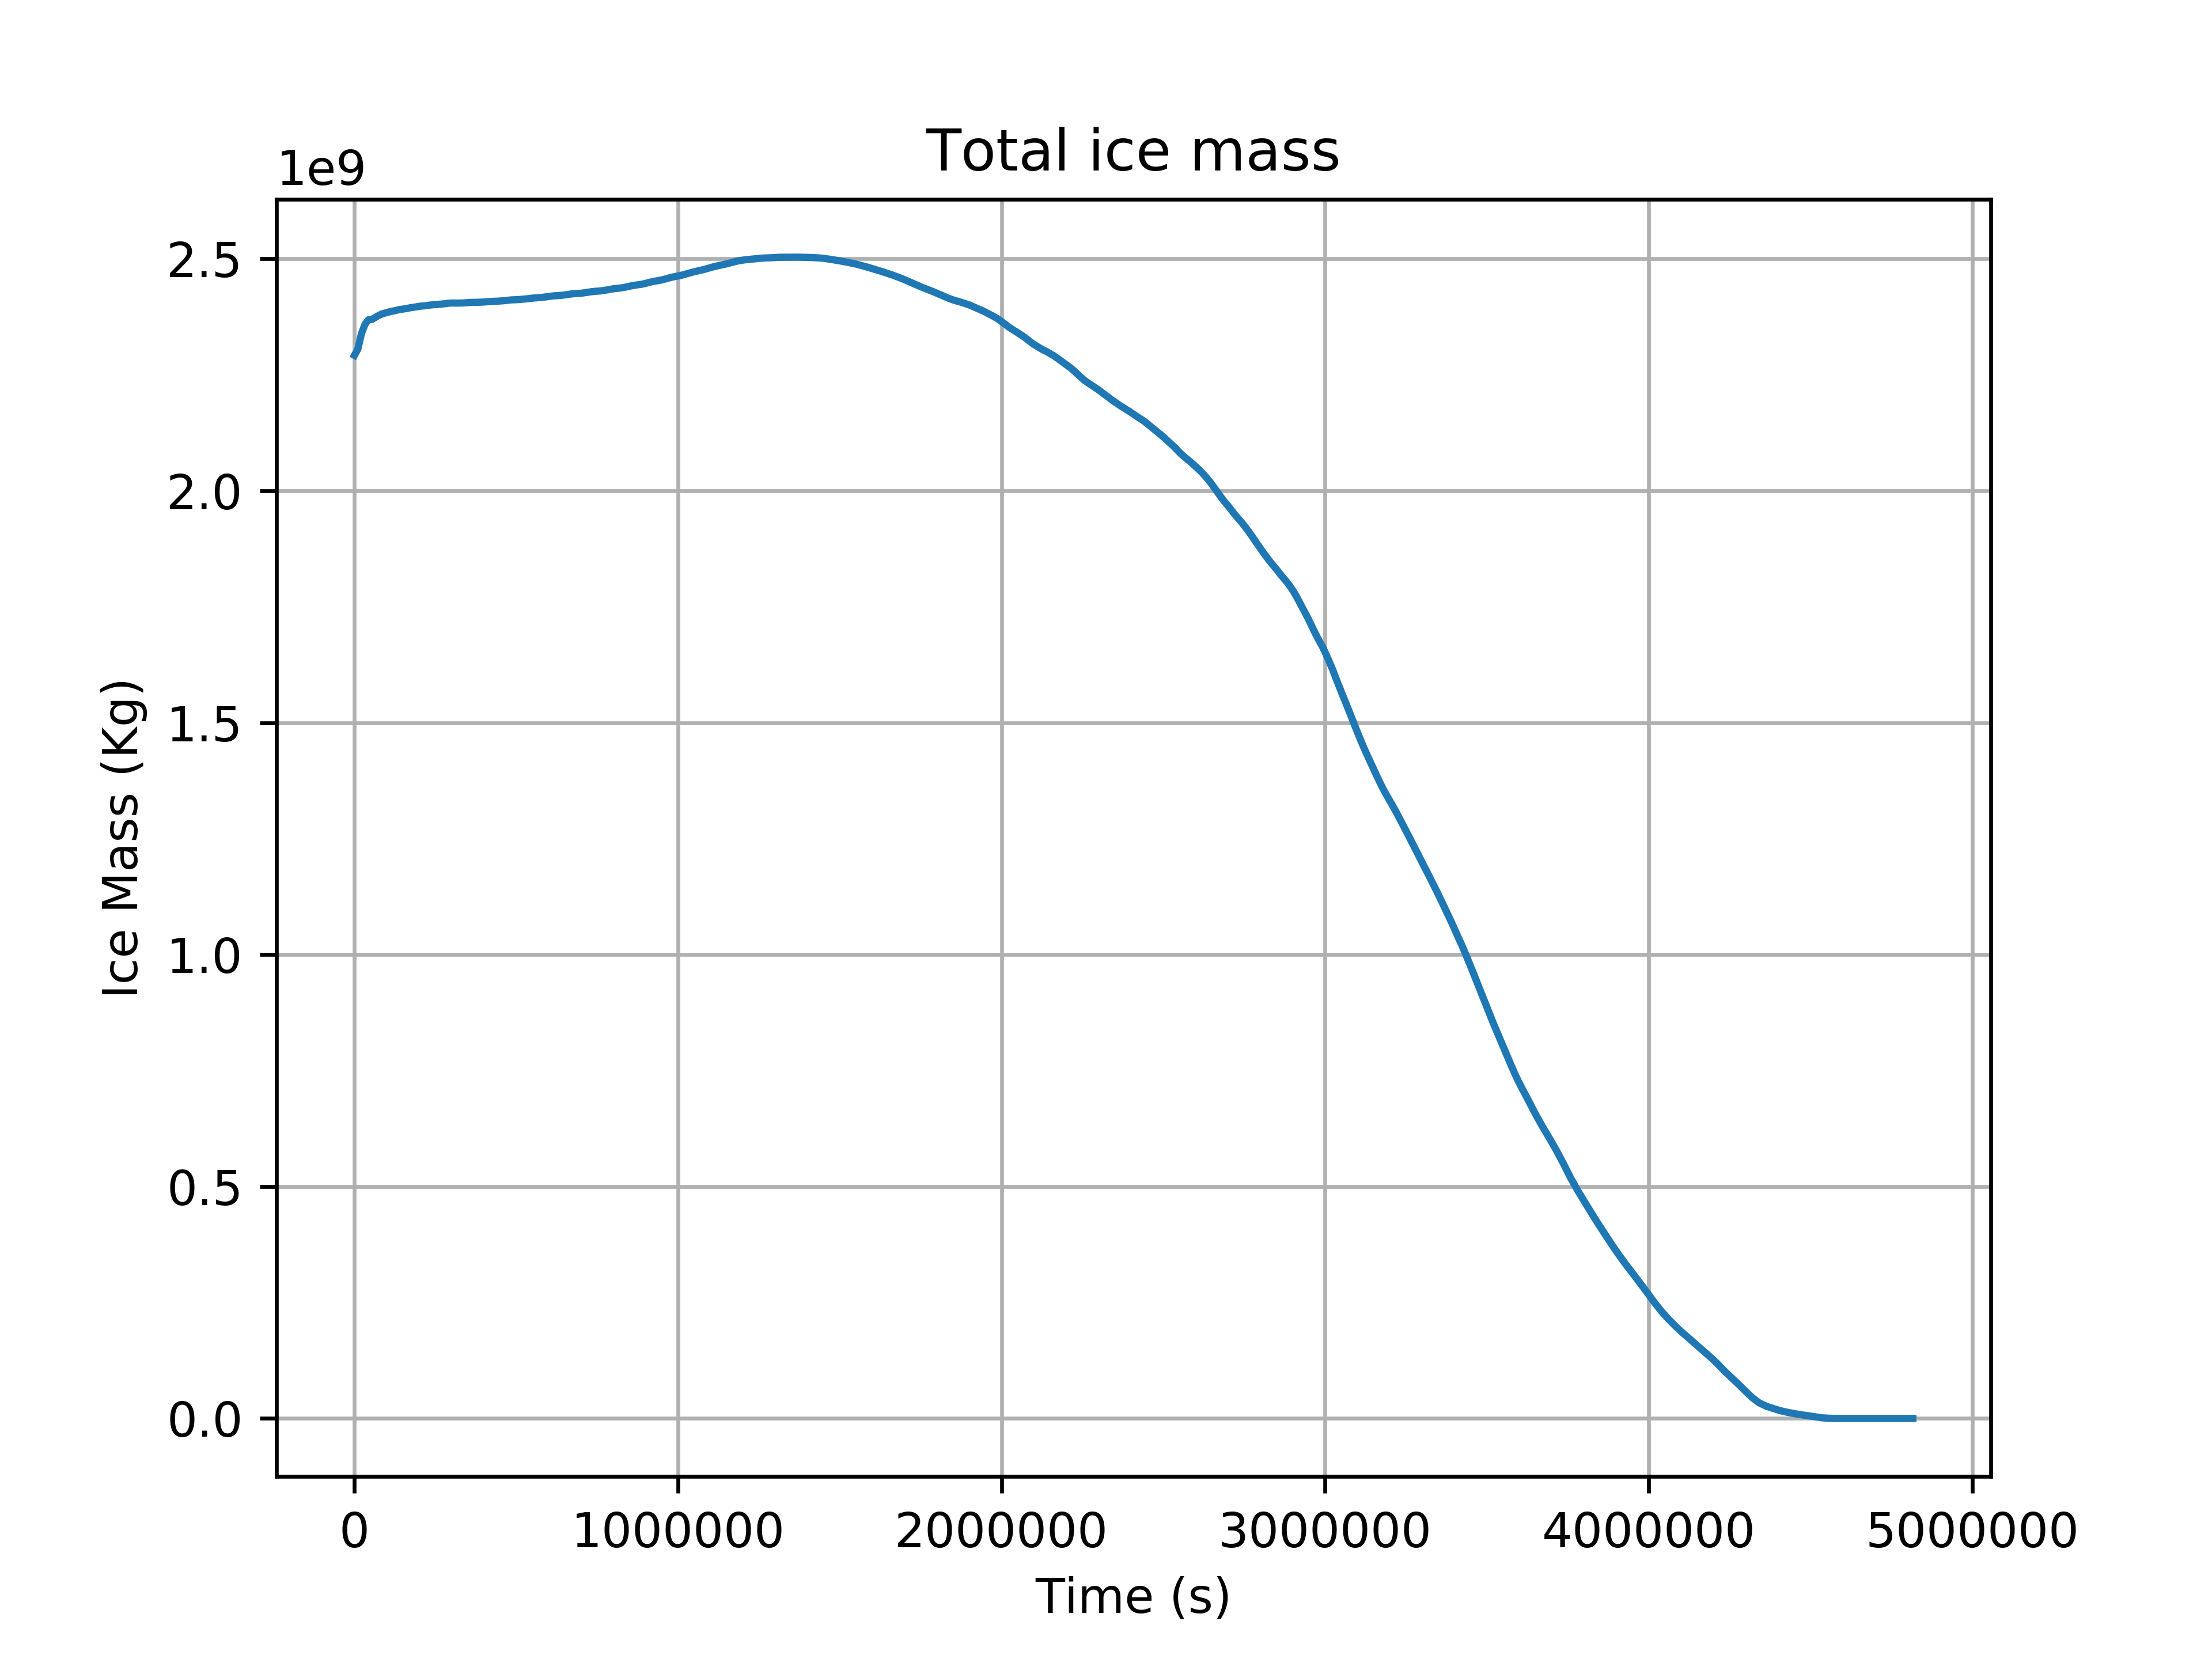
\includegraphics[width=0.8\linewidth]{iceMelt/icemeltsmooth-icemass}
\caption{Total ice mass for case 2. The ice initially grows in the cold water, and later is melted by the warm air temperature and solar radiation.}
\label{fig:iceMelt0IceMass}
\end{figure}

\clearpage
\begin{figure}[h!]
\begin{subfigure}{0.8\linewidth}
\centering
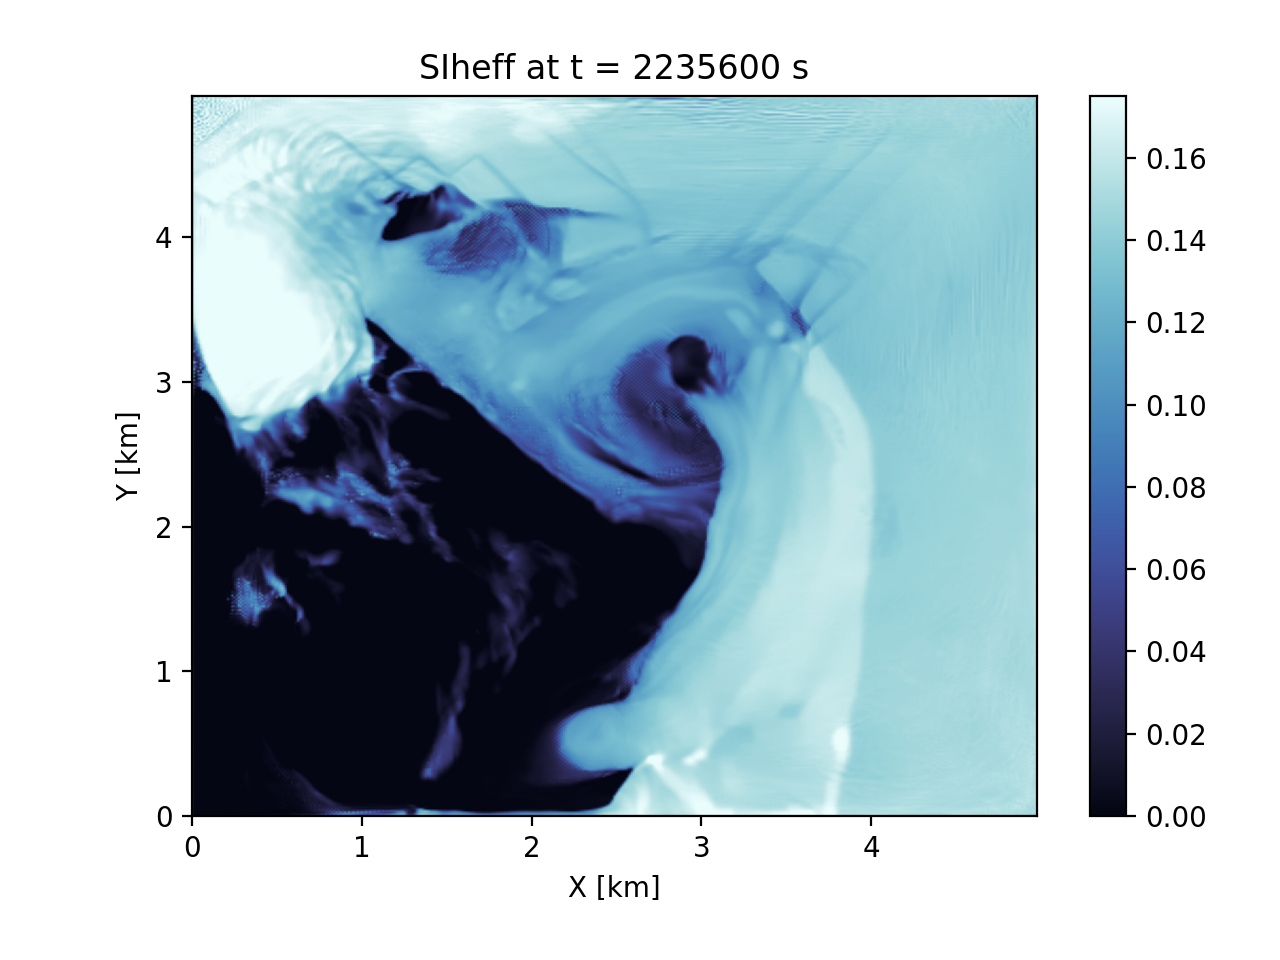
\includegraphics[width=\linewidth]{iceMelt/icemeltsmooth-surface-ice-thick-0001117800}
\end{subfigure}
\begin{subfigure}{0.8\linewidth}
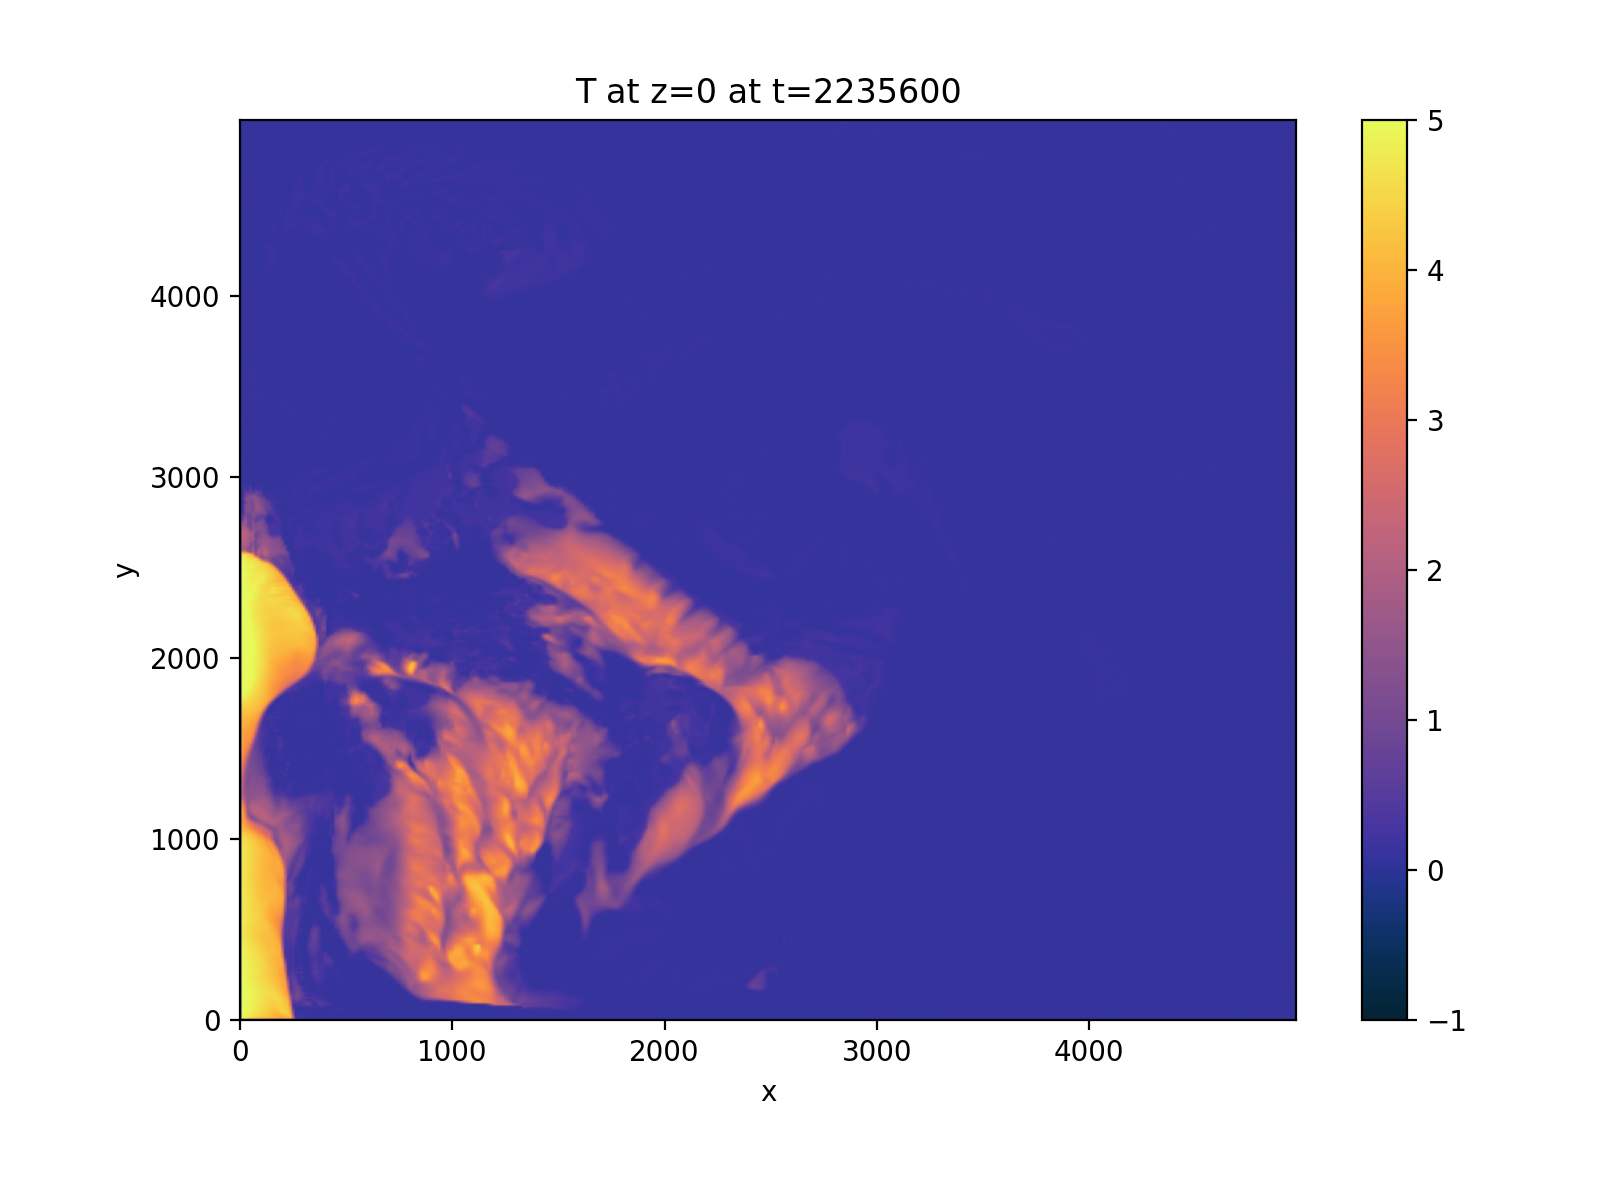
\includegraphics[width=\linewidth]{iceMelt/icemeltsmooth-surface-T-0001117800}
\end{subfigure}
\caption{Effective ice thickness (top) and surface temperature (bottom) for case 2. The ice has melted in the bottom left corner from the wind. Notice the ridge built up to the right of the open water, and the cracking in the ice above the open water.}
\label{fig:iceMelt0}
\end{figure}

\subsubsection*{Parameter comparisons}
We want to see how sensitive the results are to changes in some parameters. We compare
\begin{itemize}
\item{Hydrostatic and non-hydrostatic model configurations}
\item{Higher resolution}
\item{Removing surface winds}
\end{itemize}
The model runs much faster in hydrostatic configuration than non-hydrostatic, and eventually we will need to use the hydrostatic configuration to run a full lake-scale model. Therefore, we'd like to know how much of a difference this approximation makes for our cases. Similarly, we want to understand what impact resolution will have in our simulations. Therefore, we run 4 cases: high and low resolution for both hydrostatic and non-hydrostatic configurations. We start with 12.5 m horizontal resolution, and increase to 6.25 m resolution. Total kinetic energy in the water (not including kinetic energy of the ice) is compared in figure \ref{fig:iceMeltCompareTKE}. The case with no surface wind is not shown since the kinetic energy is significantly lower.

\begin{figure}[h!]
\centering
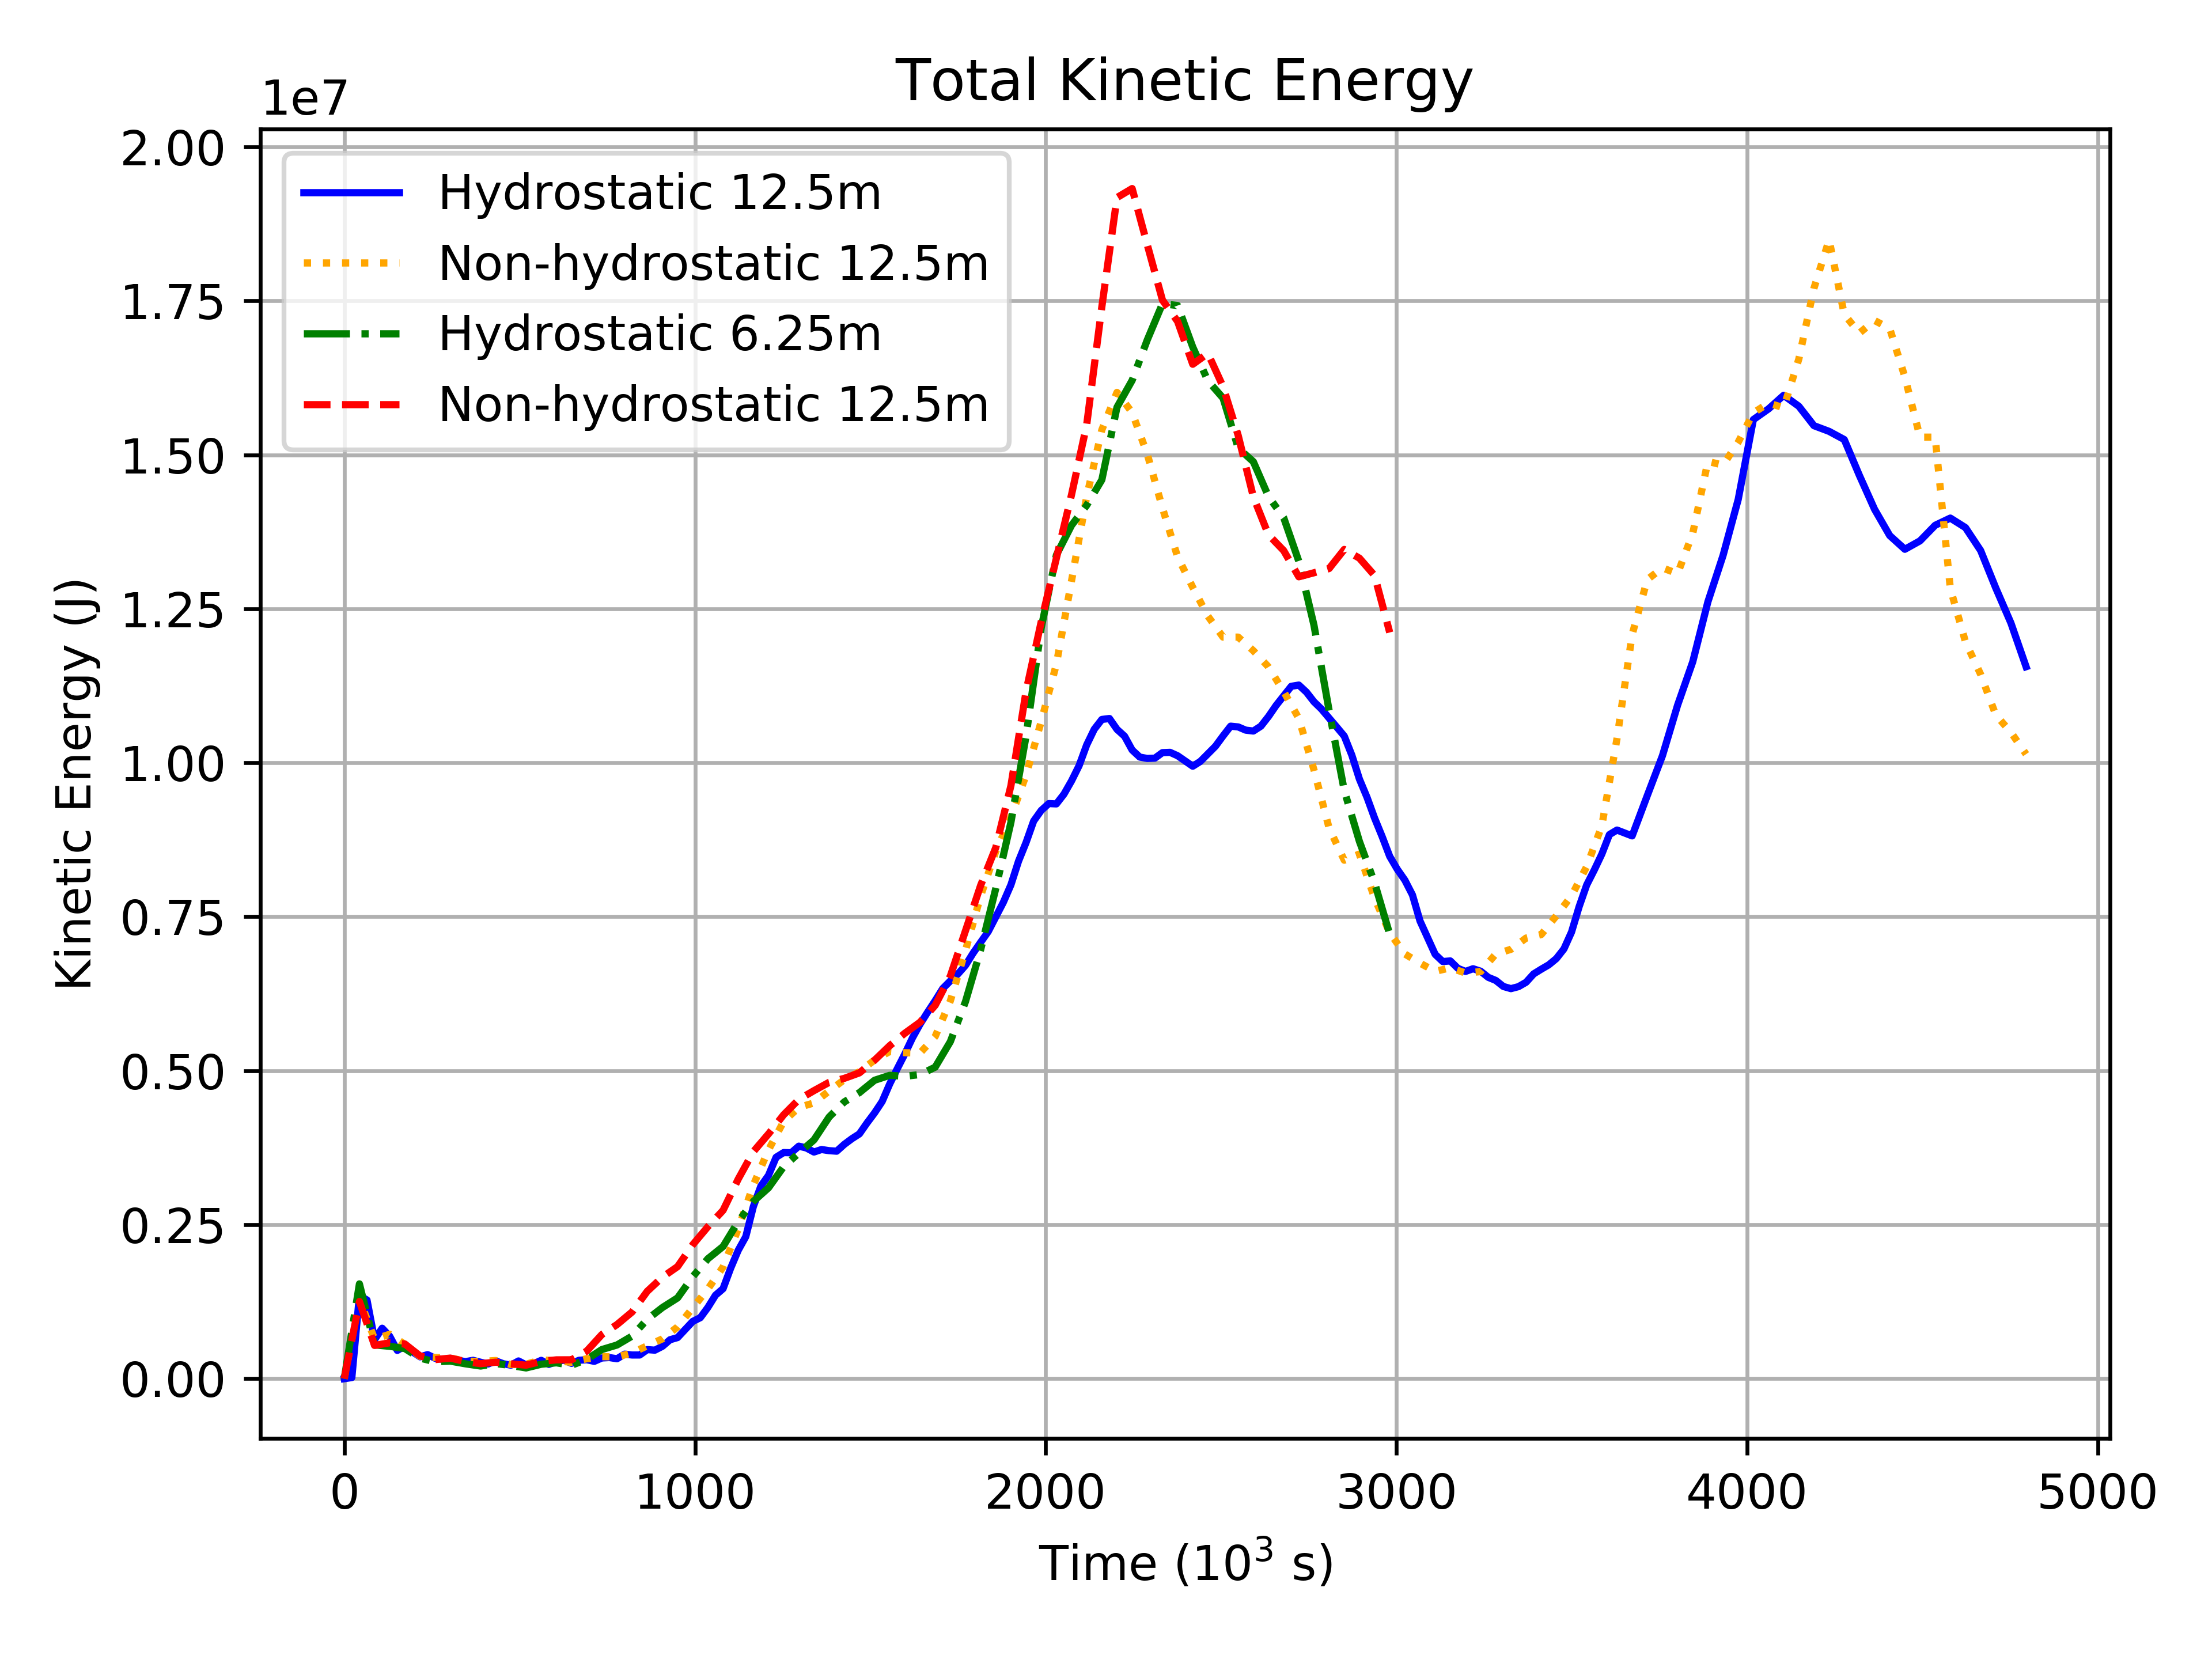
\includegraphics[width=0.85\linewidth]{iceMelt/icemeltsmooth-deltaTKE}
\caption{Case 2: Comparison of total kinetic energy of the water for different model configurations.}
\label{fig:iceMeltCompareTKE}
\end{figure}

The high-resolution simulations have good agreement between hydrostatic and non-hydrostatic configurations, and agree well with the lower resolution non-hydrostatic configuration. The low resolution hydrostatic configuration underestimates the first maximum of kinetic energy compared to the other simulations.

We can compare the mean ice thickness and total internal energy in the water between model configurations. We compare the above simulations, as well as the simulation with no surface winds. Intuitively removing the winds should change the rate of heat transfer and ice break-up, so we investigate this. The results are in figure \ref{fig:iceMeltCompareWinds}.

In each case, the ice melts most rapidly at about 5 weeks into the simulation. Call this the break-up time. All simulations have relatively good agreement on ice thickness until the break-up time. The case with no wind takes longer to start melting, and then melts faster, than the other cases. At break-up time the case with no wind seems to be able to transfer heat from the water into the ice to melt it more efficiently than the other cases. There could be more evaporative cooling in the water when there are now winds, which could be a possible mechanicsm for the different warming rates. This might explain the dip in internal energy compared to the other cases.

\clearpage
\begin{figure}[h!]
\begin{subfigure}{0.95\linewidth}
\centering
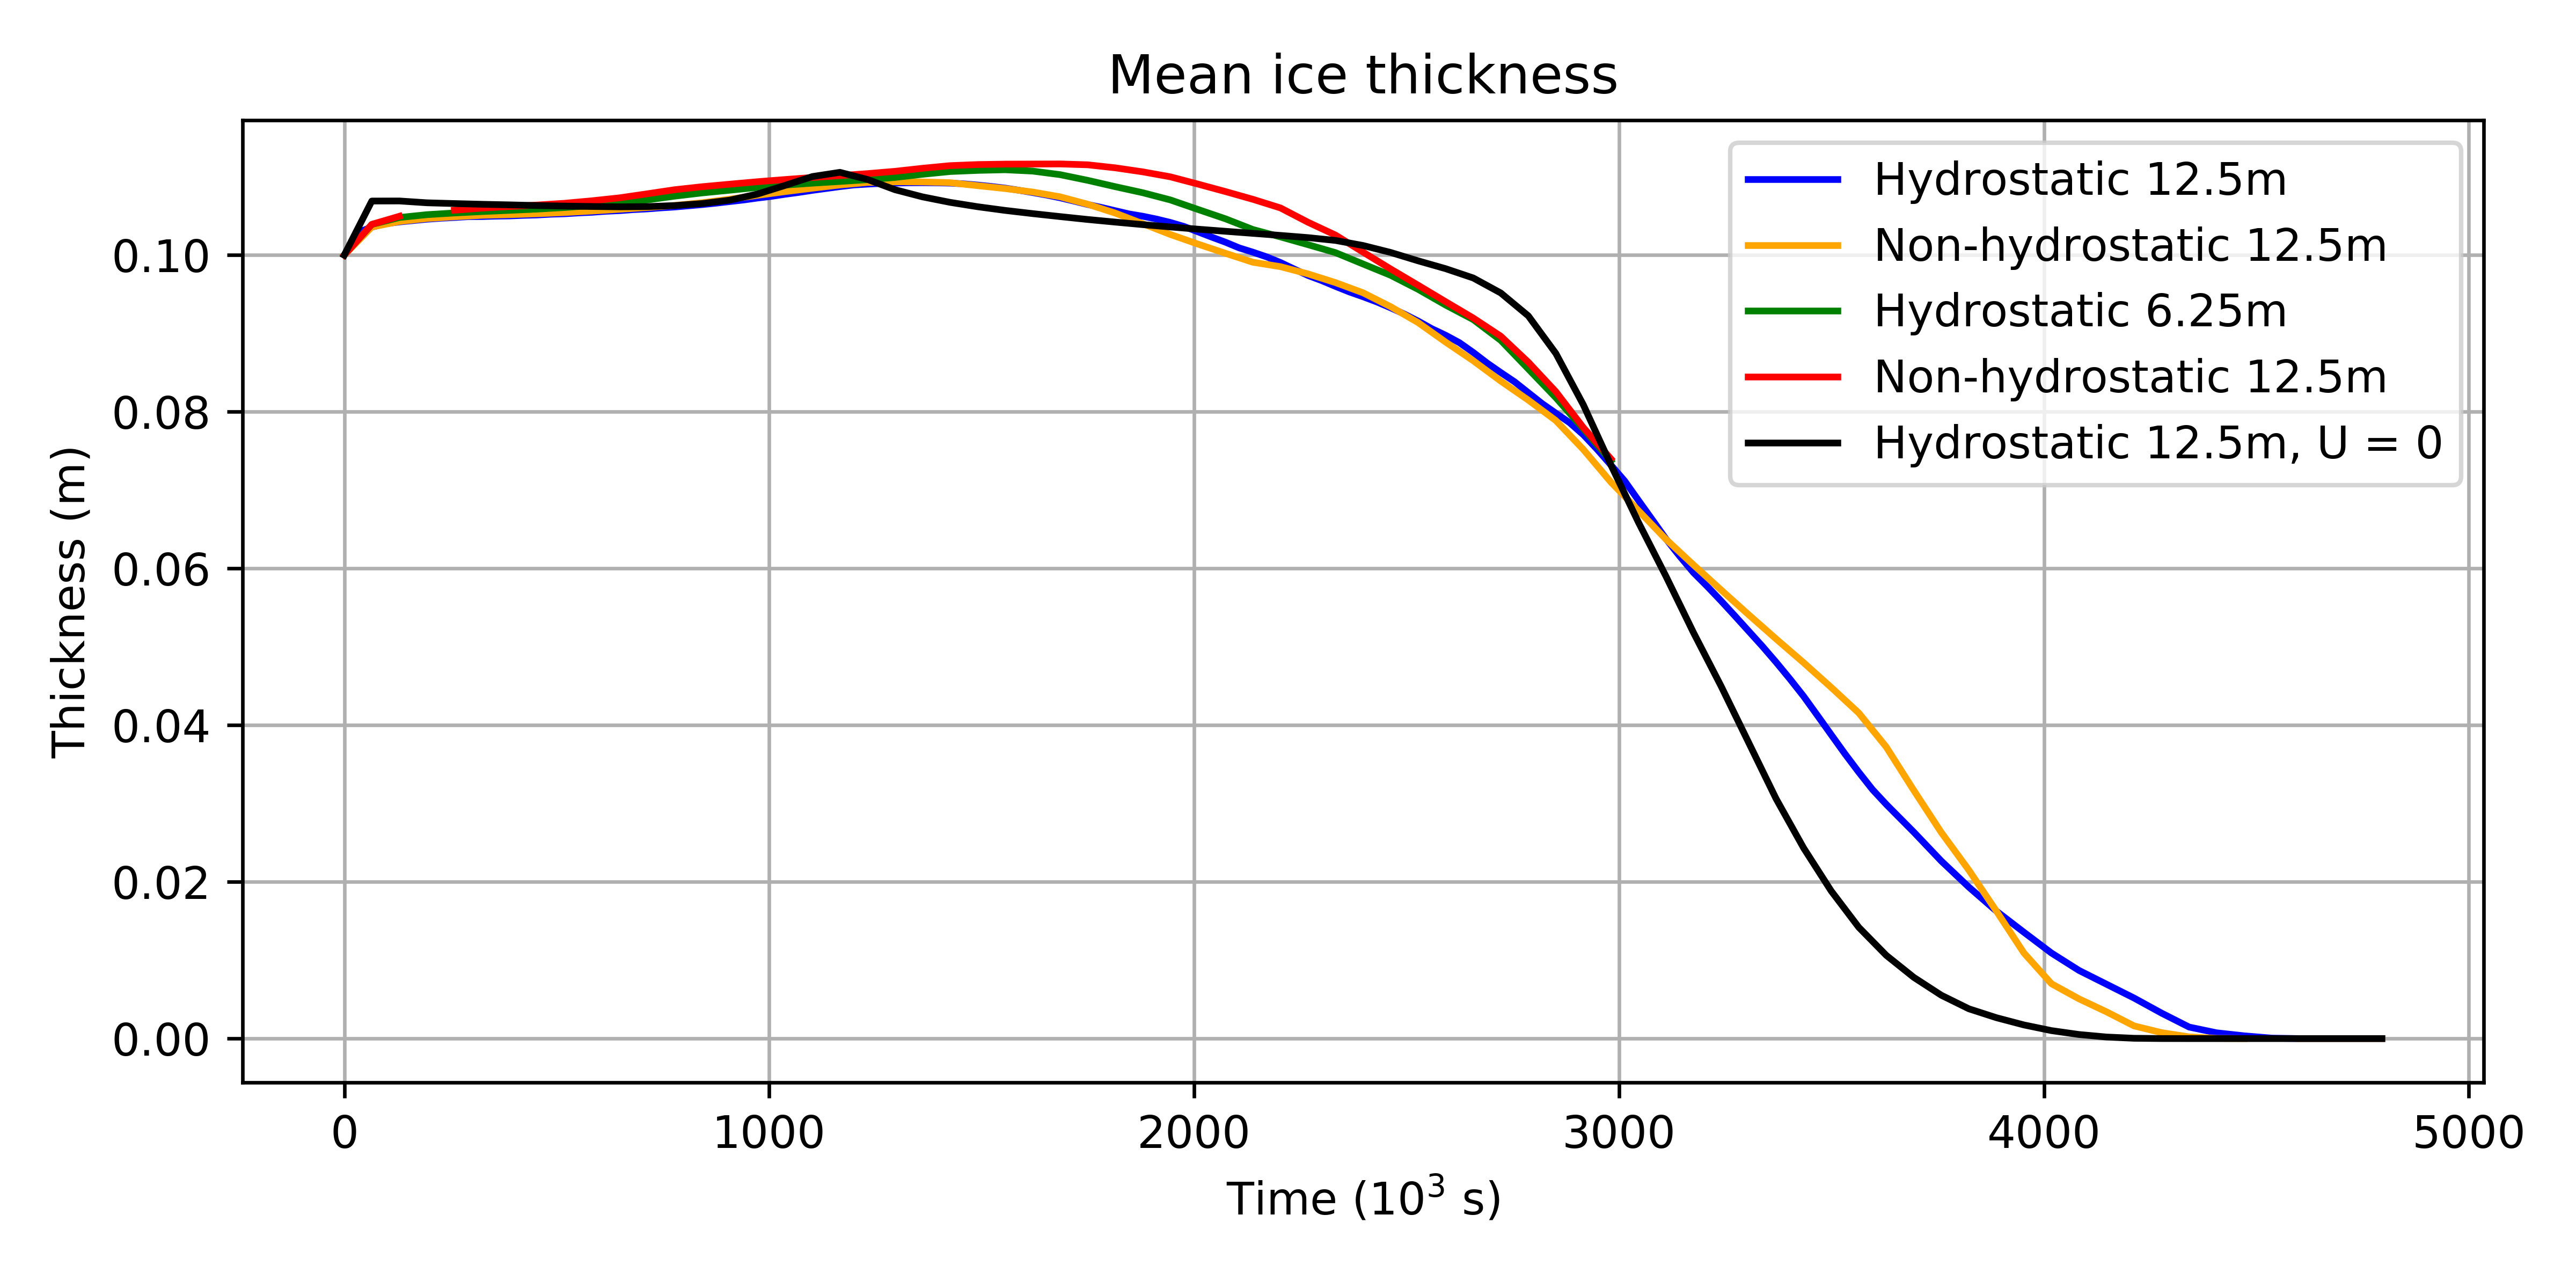
\includegraphics[width=\linewidth]{iceMelt/icemeltsmooth-deltaIce}
\end{subfigure}
\begin{subfigure}{0.95\linewidth}
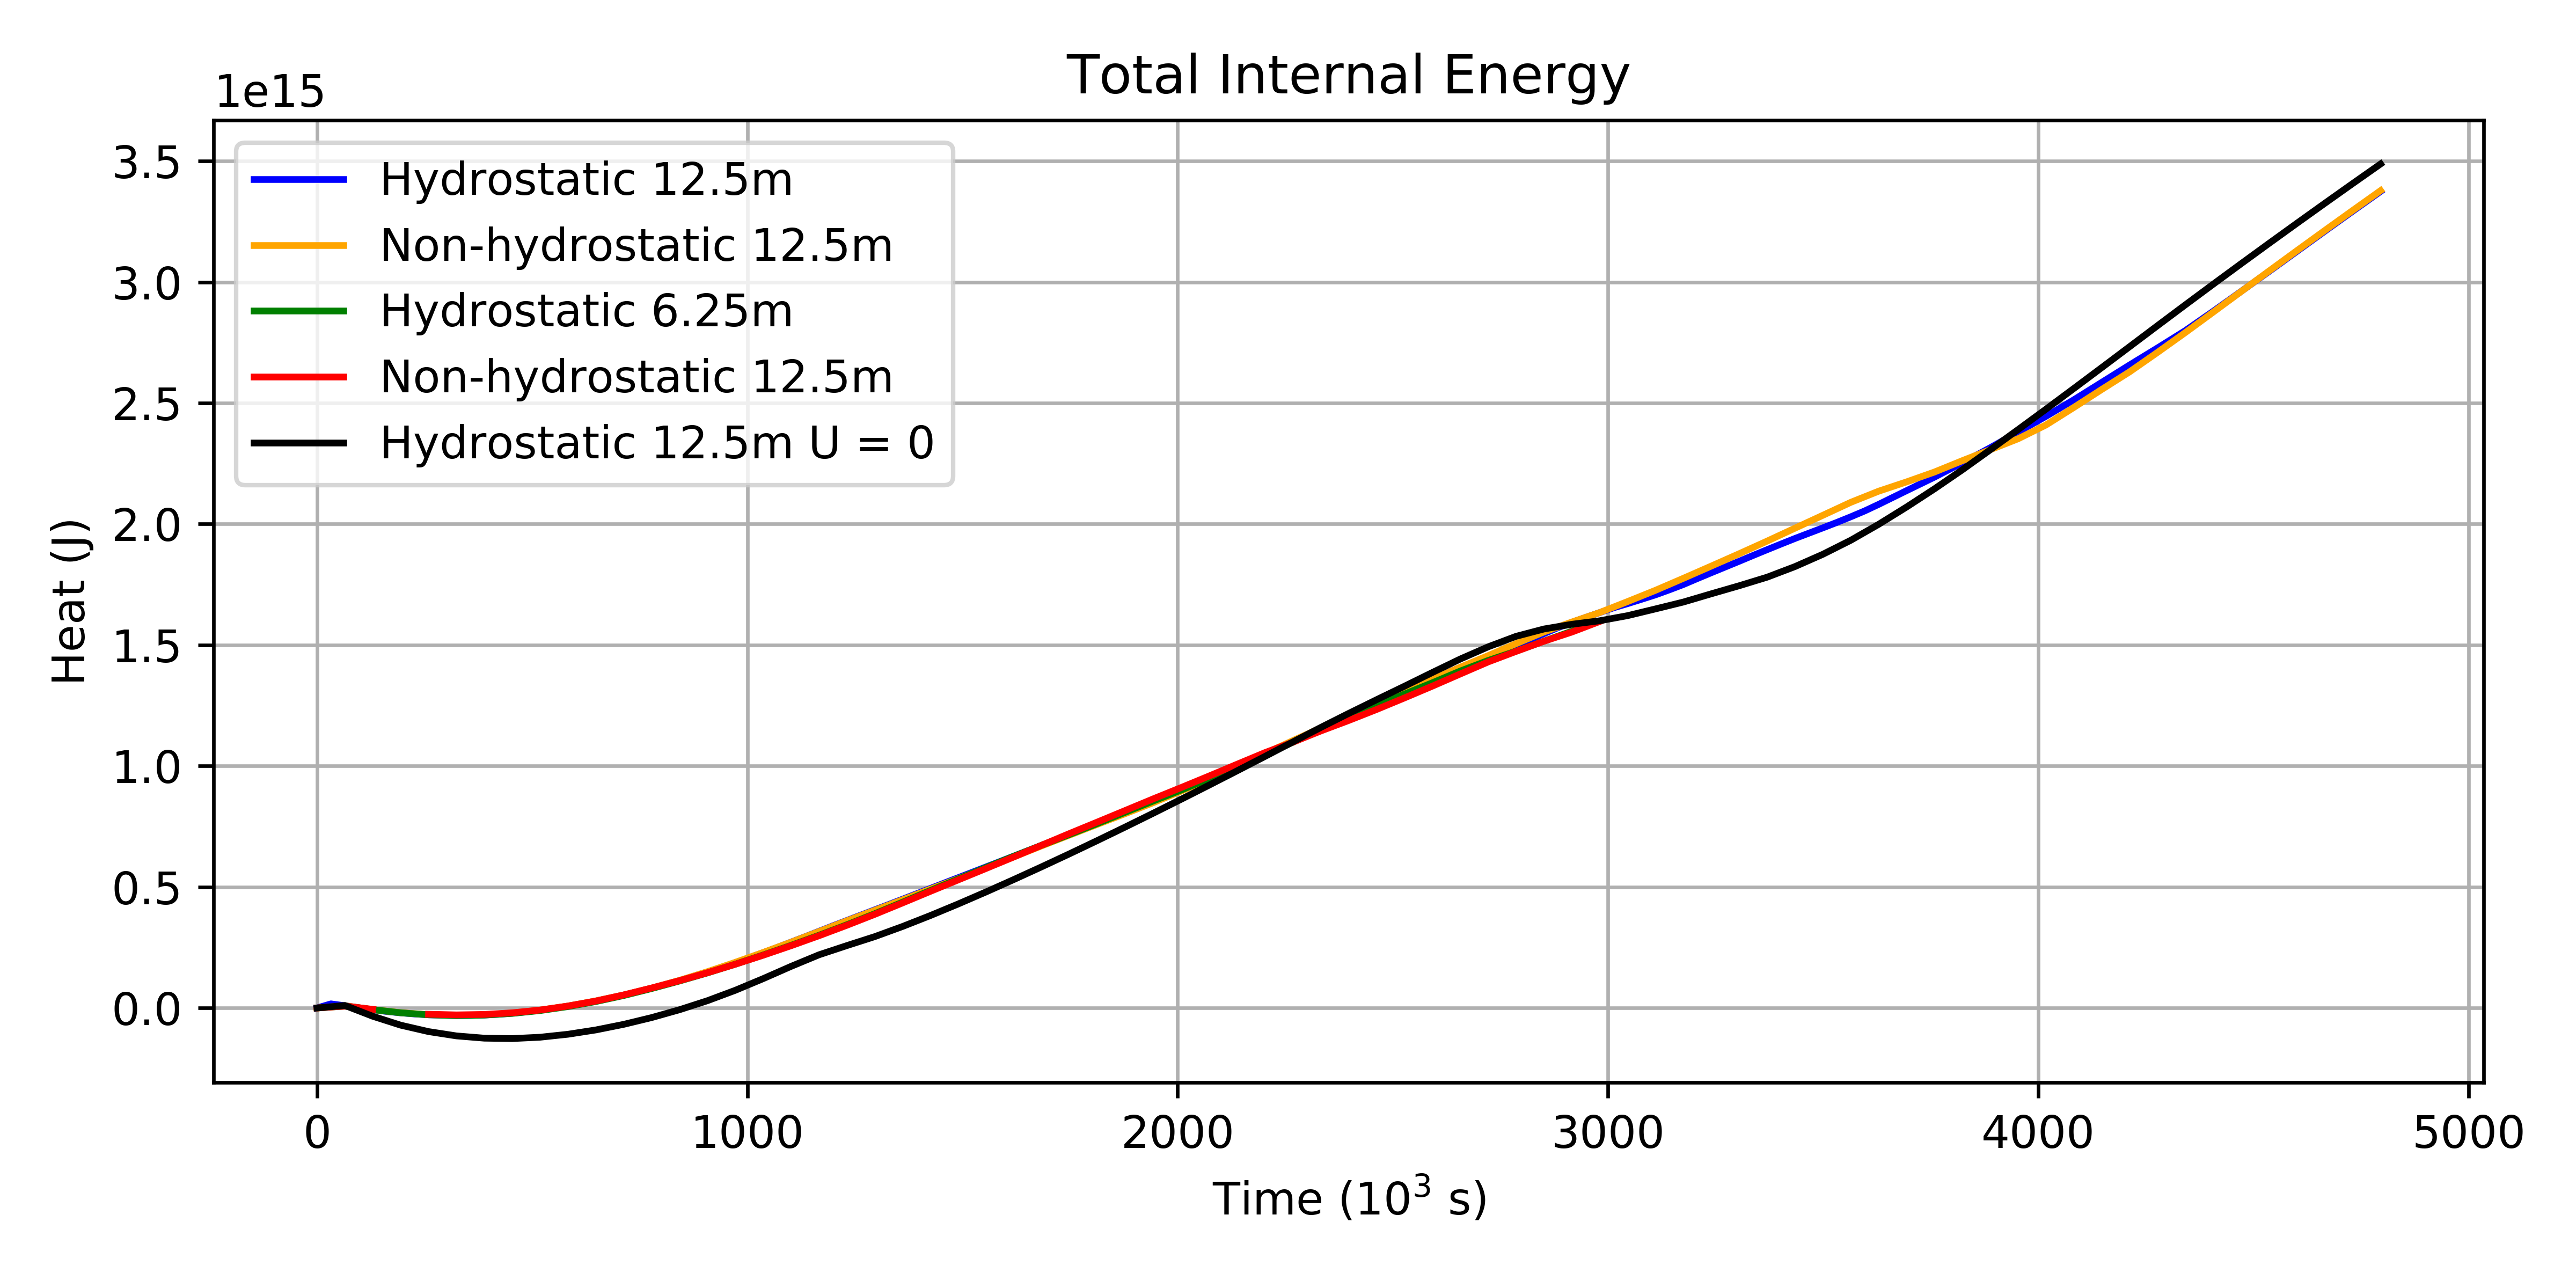
\includegraphics[width=\linewidth]{iceMelt/icemeltsmooth-deltaQ}
\end{subfigure}
\caption{Case 2: Comparison of mean ice thickness (top) and total internal energy of the water (bottom) between model configurations.}
\label{fig:iceMeltCompareWinds}
\end{figure}

The case with no surface wind has very different qualitative ice distributions when it melts than the case with surface wind (fig \ref{fig:iceMeltNoWind}). The ice mostly melts from the edges, but still forms coherent clumps. It maintains a more even distribution throughout the domain, which may contribute to melting faster. The spatial variability seen in figure \ref{fig:iceMeltNoWind} is likely from noise in the numerics. MITgcm is a finite volume formulation which will introduce some noise into the solution.

\begin{figure}[h!]
\centering
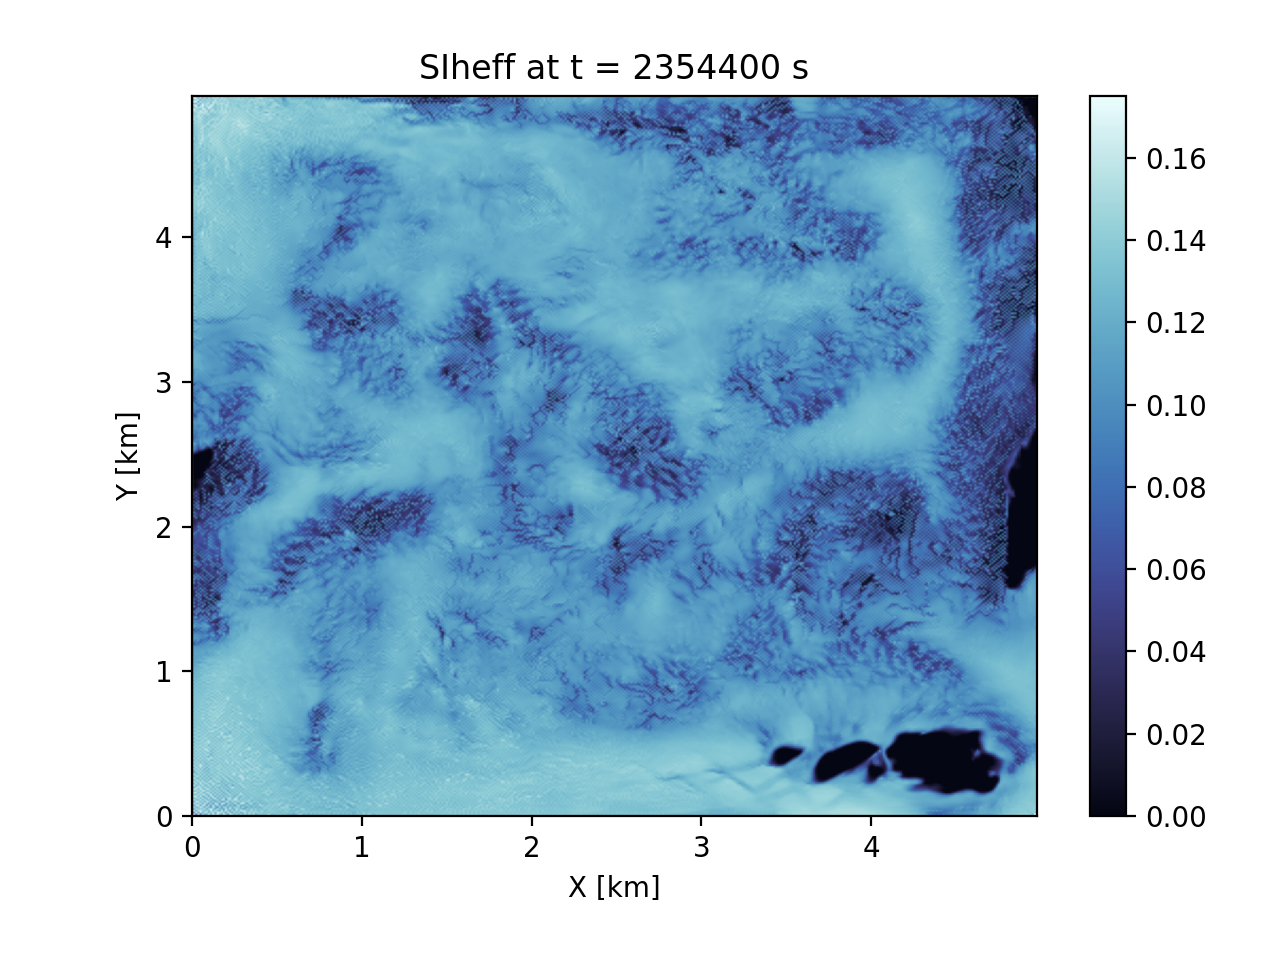
\includegraphics[width=0.9\linewidth]{iceMelt/icemeltsmooth-nowind-surface-ice-thick-0001177200}
\caption{Surface ice thickness for case 2 with no surface winds. The ice largely melts from the edges, with some spatial variability}
\label{fig:iceMeltNoWind}
\end{figure}

\subsubsection{What was learned}
From running the main case, we can say the model melts ice reasonably physically. The ice melts until it gets thin enough to break up, at which point it cracks and starts being pushed around by the wind and surface currents. The ice continues to move and melt, eventually melting entirely. The remaining water is heated by the downward radiation and warm air temperature.

The total kinetic energy varies significantly between different parameter sets. In particular, the kinetic energy is significantly different between hydrostatic and non-hydrostatic configurations at lower resolutions. This could be a problem for lake scale simulations, where the resolution would be relatively large. However, we expect that for large resolutions the difference between hydrostatic and non-hydrostatic configurations should be small. Nevertheless, even with the large difference in kinetic energy, the total internal energy and average ice thickness are relatively insensitive to changing the hydrostatic flag. They are more sensitive to the inclusion of surface winds, which may be expected.

Regarding running the model, I had to include a very small wind speed instead of truly 0 winds. This is discussed in more detail in section \ref{sec:epsilonWinds}. These cases were also run without all the recommended modifications to the default parameters given in listing \ref{listing:seaiceDefaults}. These results should be checked with those improved parameters and flags.

\subsubsection{Next steps}
This case with the same initial conditions has been studied thoroughly. It could be worthwhile to compare the melting rate to initial conditions with some small variability in the initial ice distribution, which is more realistic. This could also be a good case to introduce more interesting bathymetry and see what effect lake shape has on the dynamics.

\subsection{Case 3: Solar forcing}
We are interested in how the model simulates solar forcing over open water and ice covered water. This is clearly important to lake dynamics, and likely needs to be studied in more detail than I have done so far.

To study the different solar forcing for ice-covered and open water, I initialize a lake to be completely covered in $\SI{1}{m}$ thick ice in the north half and open water in the south half. This is an idealized interface between an ice sheet and open water in a real lake. I set the air temperature to be $\SI{0}{\celsius}$, and send down $\SI{300}{W.m^{-2}}$ of both shortwave and longwave radiation. I continue to use eastward winds in only the south half of the lake. See more details on the setup in table \ref{table:solarForcing}.

From this case, I want to see
\begin{itemize}
\item{More warming in the open water than under ice covered water, since the ice should reflect most of the incoming radiation and absorb heat from the water in melting}
\item{A layer of cold water staying under the ice since the water at $\SI{0}{\celsius}$ is less dense than sun-heated water closer to $\SI{4}{\celsius}$}
\end{itemize}

\begin{longtable}{  p{.30\textwidth}  p{.30\textwidth}  p{.4\textwidth}  }
\hline
\textbf{Paramter Name} & \textbf{Parameter Value} & \textbf{Comment} \\ \hline \hline
\verb|Nx| & 600 & 50 x 12 processors \\ \hline
\verb|Ny| & 600 & 50 x 12 processors \\ \hline
\verb|tempAdvScheme|	&	33	&	High order advection scheme \\ \hline
\verb|nonHydrostatic| & \verb|.FALSE.| & Hydrostatic model configuration \\ \hline
\verb|eosType|		&	JMD95z	&	Polynomial approximation to true equation of state. This EOS respects the max in density at $4^{\circ} \textrm{C}$\\ \hline
\verb|delX|			&	\verb|600*10.0|	&	6 km lake, 100 m resolution \\ \hline
\verb|delY|			&	\verb|600*10.0|	&	6 km lake, 100 m resolution \\ \hline
\verb|delZ|			&	\verb|100*0.1 |	&	10 m deep lake, 0.5 m resolution \\ \hline

\verb|uwind|		&	\begin{equation*} \begin{cases} 0.5 \text{ m/s} & y \leq 3 \text{km} \\ 0 \text{ m/s} & y > 3 \text{km}   \end{cases} \end{equation*} & \\ \hline
\verb|vwind| 	& 0	& \\ \hline
\verb|atemp| 	& $0^{\circ} \text{C}$		& Constant cold air temperature \\ \hline
\verb|aqh| 		& $0.01$		&	Specific humidity \\ \hline
\verb|swdown| 	& $300 \text{ W} \text{ m}^{-2}$	& Minimum shortwave downward radiation \\ \hline
\verb|lwdown| 	& $300 \text{ W} \text{ m}^{-2}$	& Minimum longwave downward radiation \\ \hline

\verb|SEAICEuseDYNAMICS| & \verb|.TRUE.| & Allow SEAICE dynamics \\ \hline
\verb|SEAICE_area_reg|   & \verb|1.0E-5| & Ice fraction less than this will be treated as zero ice for next time step \\ \hline
\verb|SEAICE_hice_reg|   & \verb|1.0E-5| & Height cutoff \\ \hline
\verb|SEAICEadvHEFF|     & \verb|.TRUE.| & Advect effective height \\ \hline
\verb|SEAICEadvAREA|     & \verb|.TRUE.| & Advect seaice area fraction \\ \hline
\verb|SEAICEadvScheme|   & $33$			& Advection scheme 33: Flux limited direct space and time advection scheme \\ \hline

Temperature & \begin{equation*} \begin{cases} 0^{\circ} \text{C} & z = 0 \text{ m} \\ 4 ^{\circ} \text{C} & z = -10 \text{ m}   \end{cases} \end{equation*} & Temperature stratified lake \\ \hline
Initial SEAICE area fraction   & $1.0, y \geq 3 \text{ km}$ & Constant ice in North half \\ \hline
Initial SEAICE thickness    & $1.0, y \geq 3 \text{ km}$ & Constant ice in North half \\ \hline

\caption{Parameter values for case 3: solar forcing}
\label{table:solarForcing}
\end{longtable}
This case was run in hydrostatic and non-hydrostatic configuration.

\subsubsection{Results}
A plot of the surface temperature is shown in figure \ref{fig:solarForcingSurfaceT}. Figure \ref{fig:solarForcingConstantT} shows constant temperature contours. Note the warm water pushing the $\SI{0}{\celsius}$ contour up under the ice in the east end of the lake. The ripples in the contours are cased by velocity shear. Since the wind has a smooth transition (hyperbolic tangent function), the wind at the ice edge is half the magnitude of the maximum wind in the south half. The surface currents are then in the negative X direction against the ice and positive X in the bulk of the open water, creating shear.

\begin{figure}[h!]
\centering
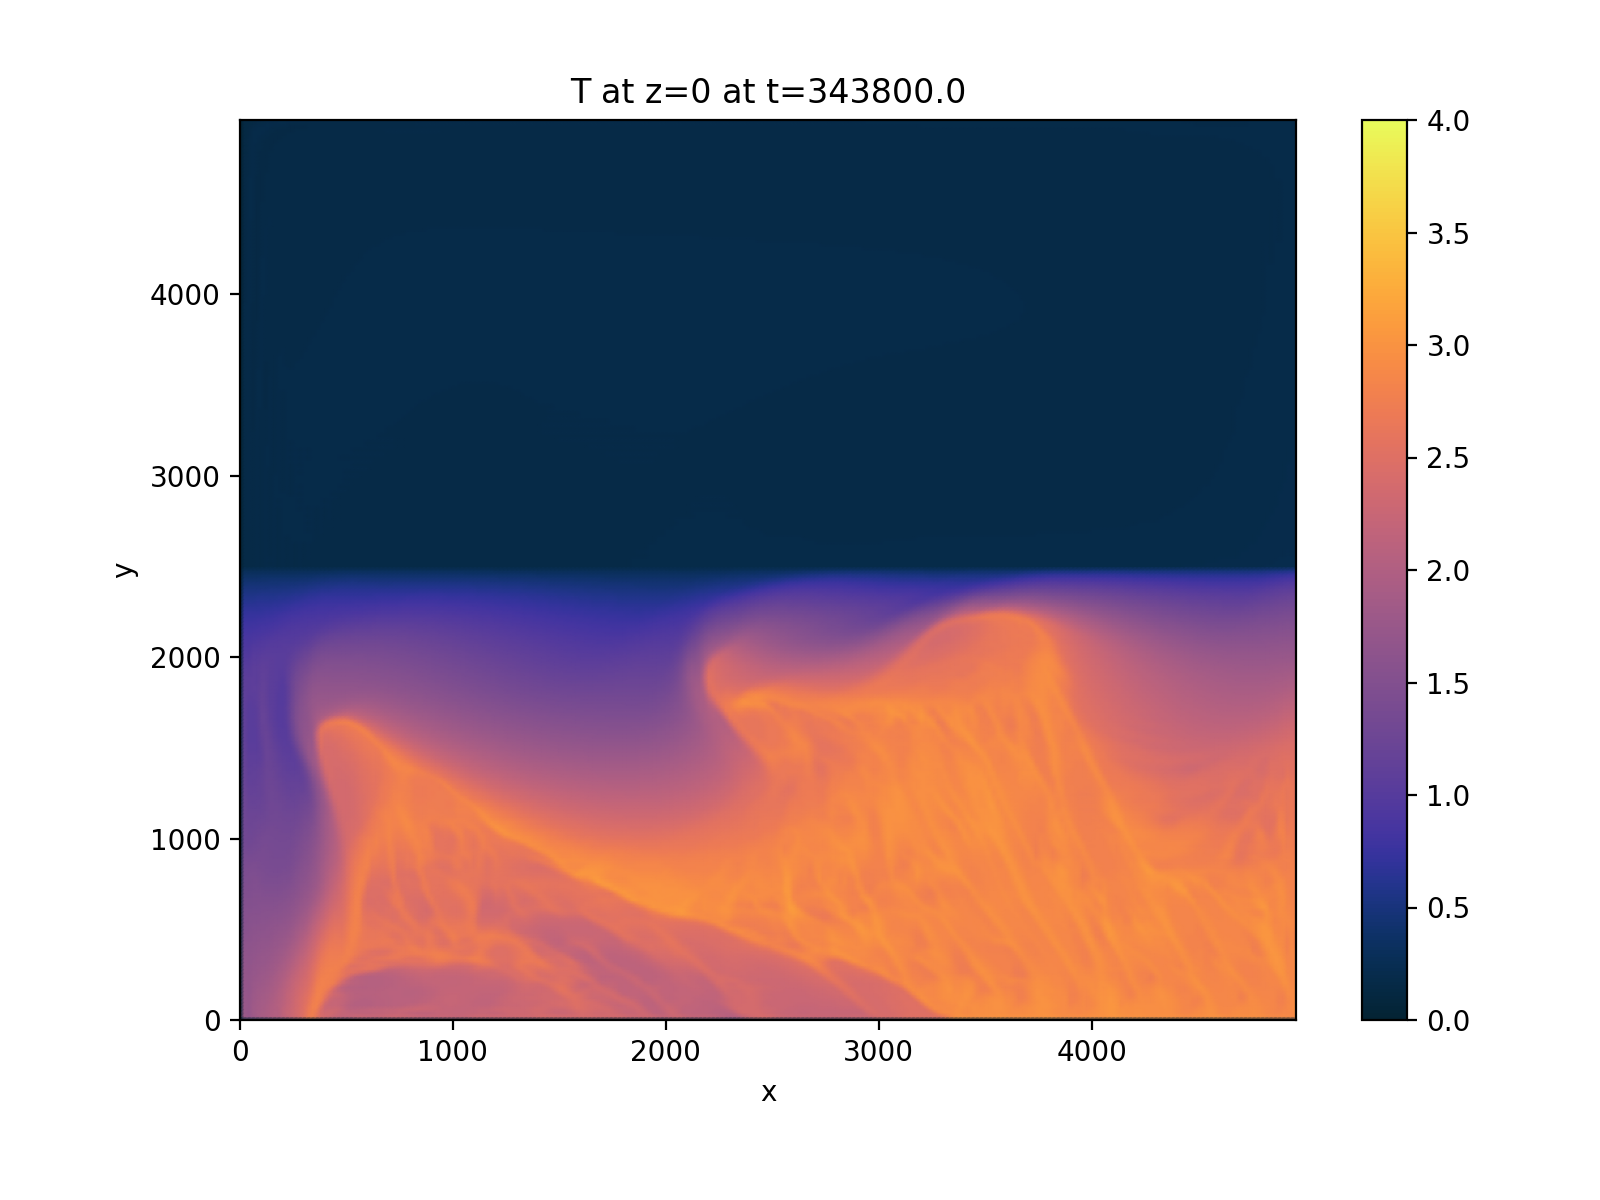
\includegraphics[width=0.85\linewidth]{solarForcing/solarforcing-surface-T-0000034380}
\caption{Surface temperature at the end of the model run for case 3. The surface layer under the ice remains at exactly $\SI{0}{\celsius}$, while the open water is warmed by the sun.}
\label{fig:solarForcingSurfaceT}
\end{figure}

\clearpage
\begin{figure}[h!]
\centering
\begin{subfigure}{0.99\linewidth}
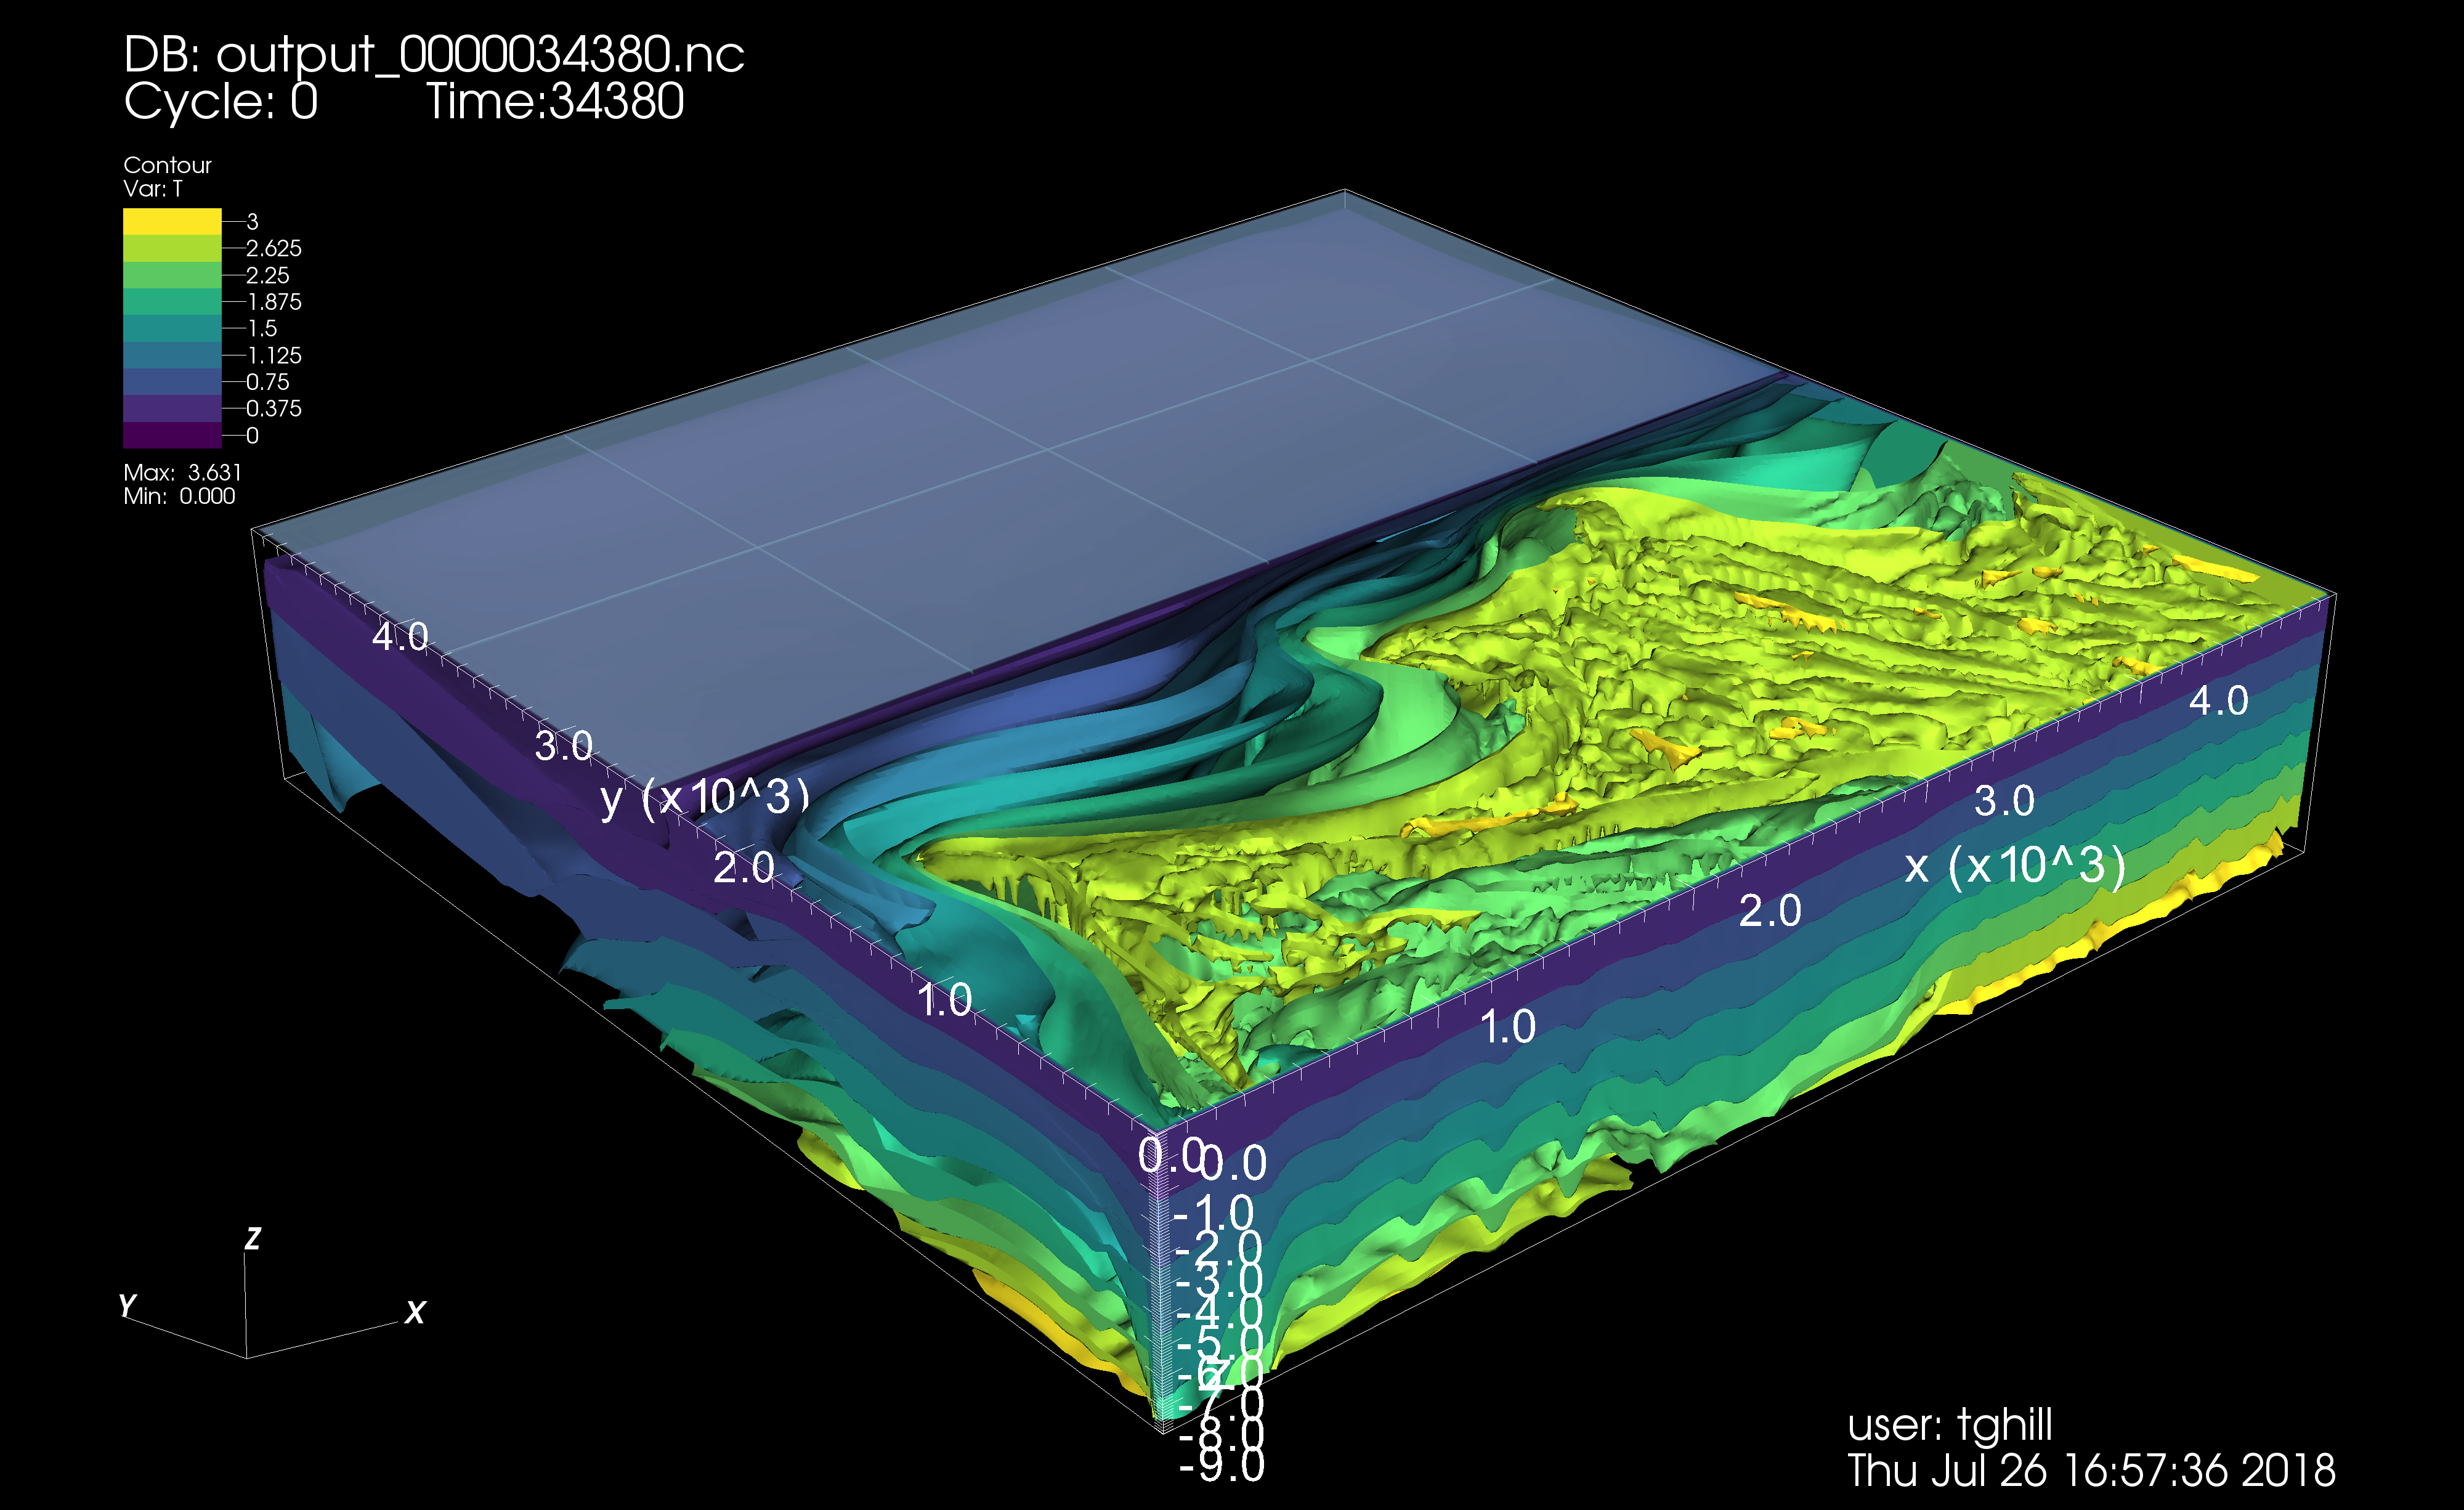
\includegraphics[width=\linewidth]{solarForcing/solarforcing-constantT}
\end{subfigure}

\begin{subfigure}{0.49\linewidth}
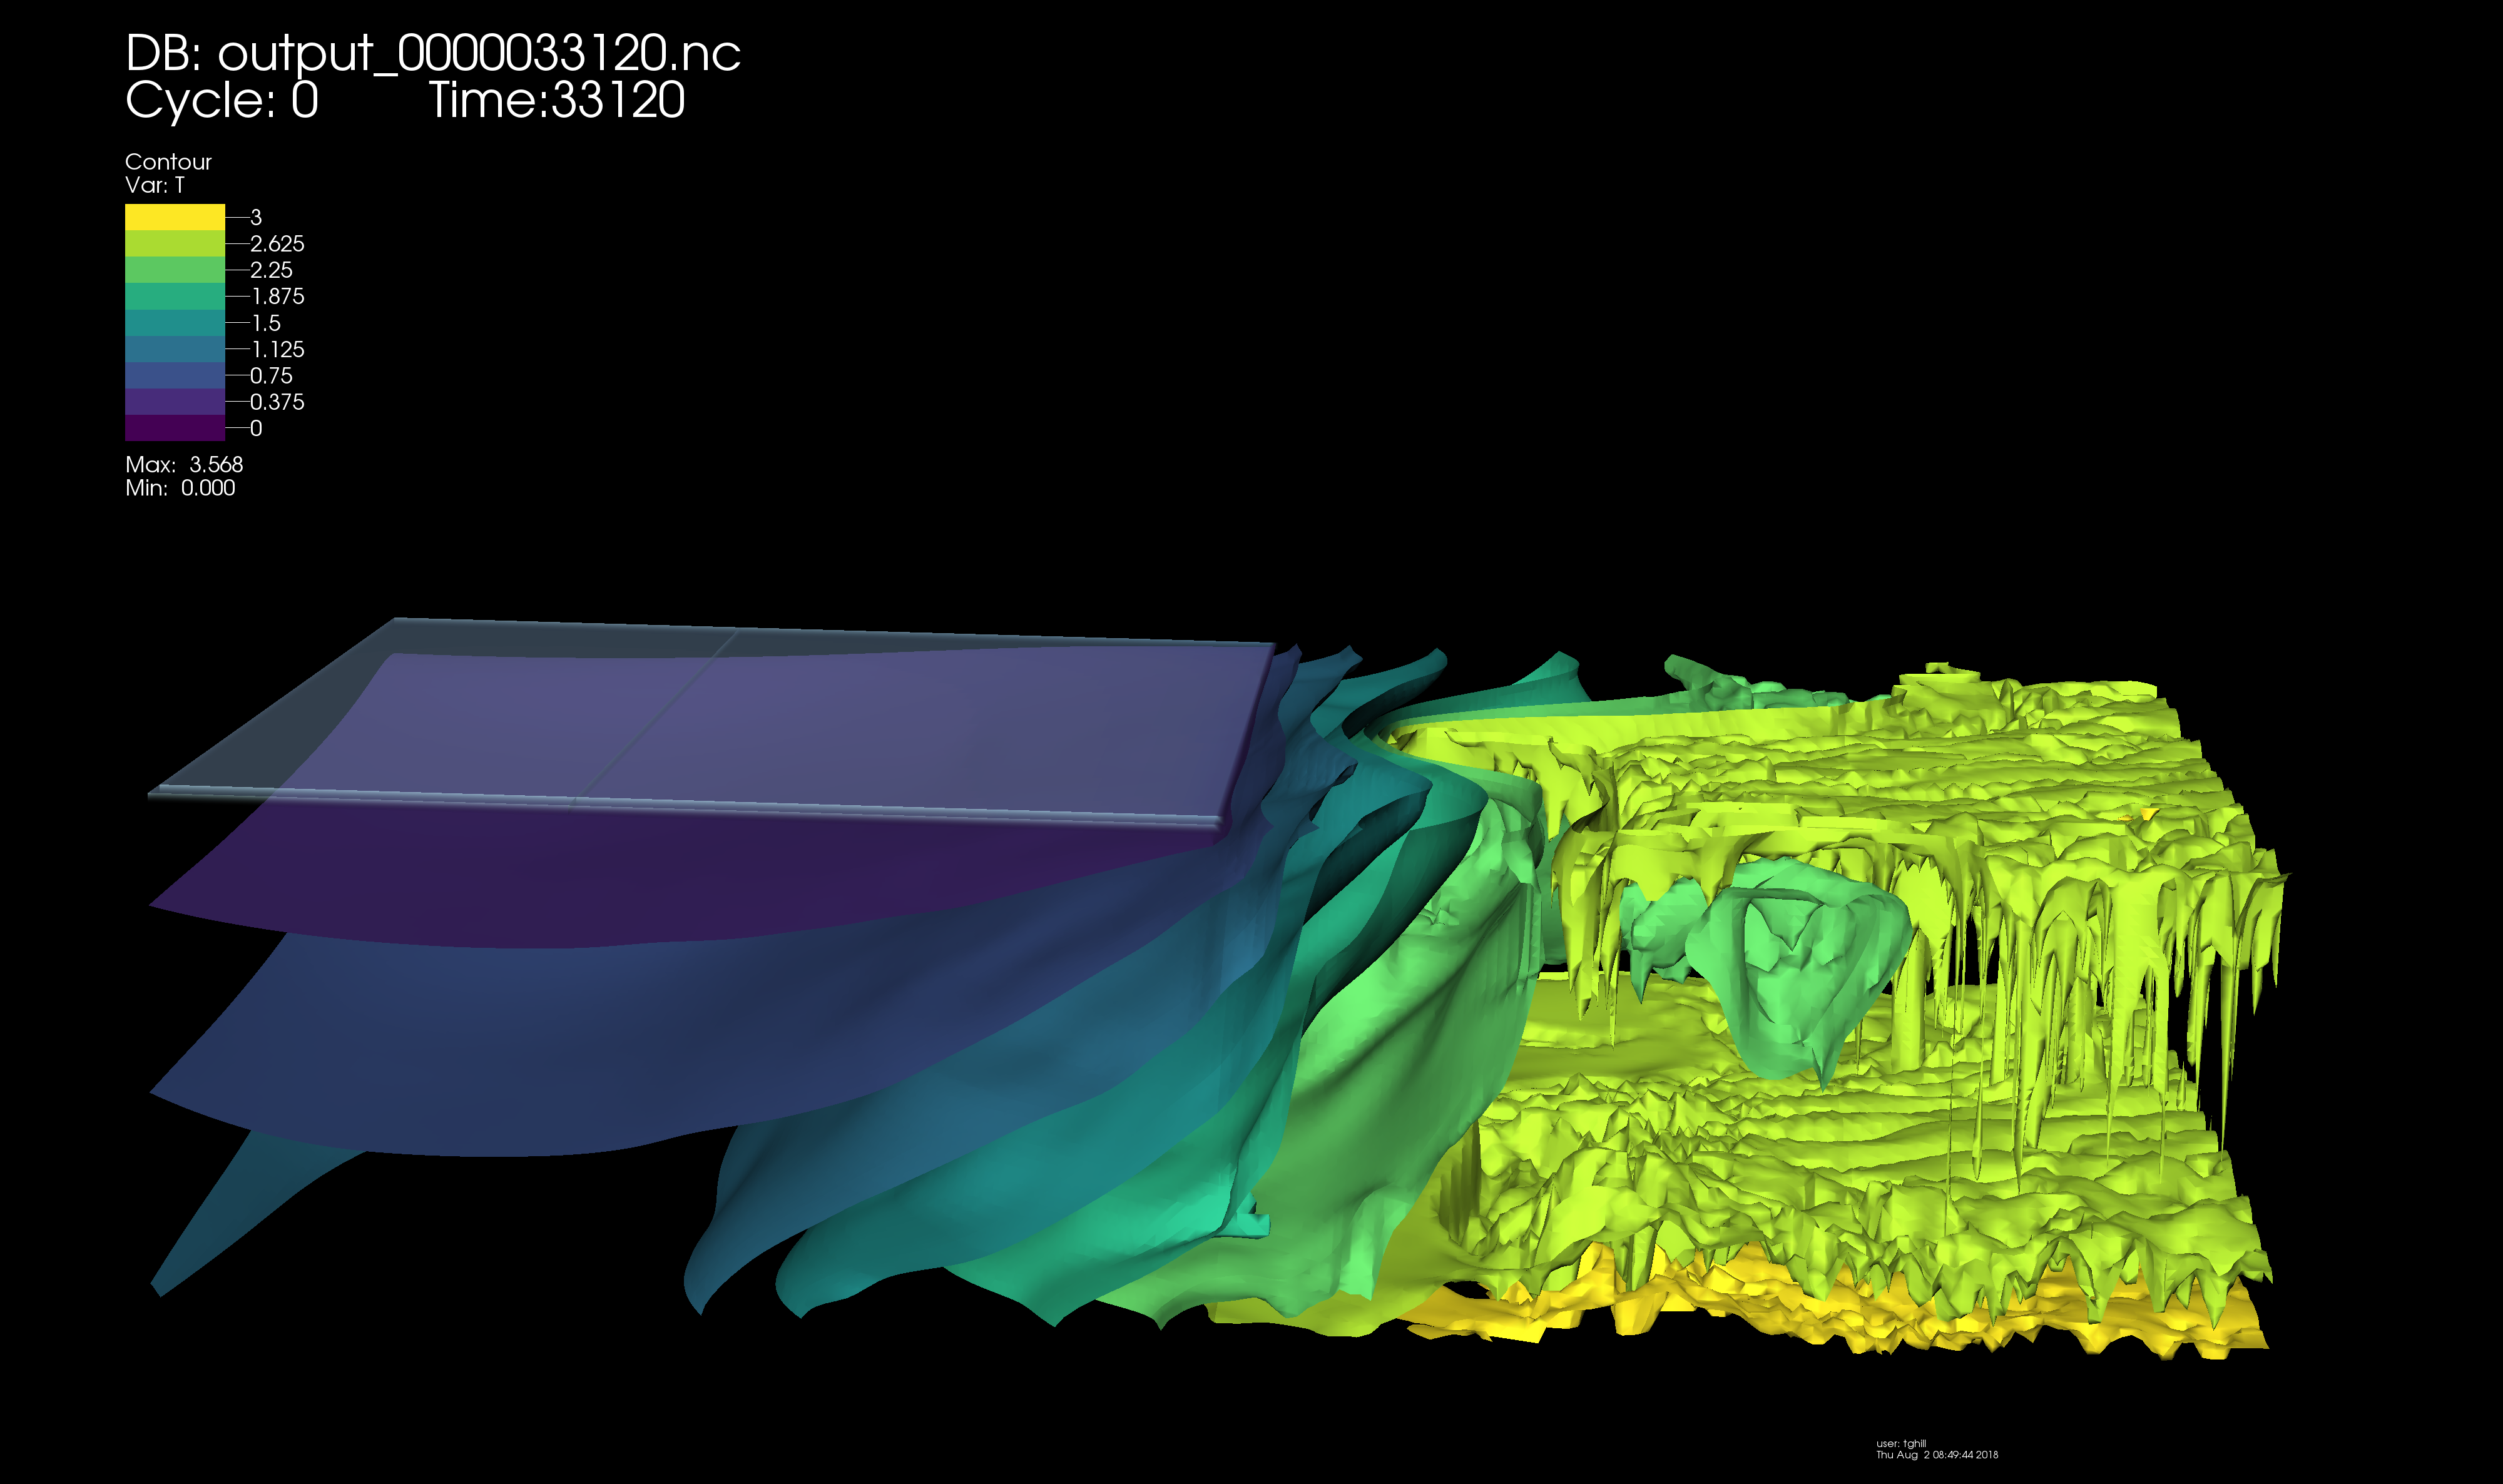
\includegraphics[width=\linewidth]{solarForcing/solarforcing-section01}
\end{subfigure}
\begin{subfigure}{0.49\linewidth}
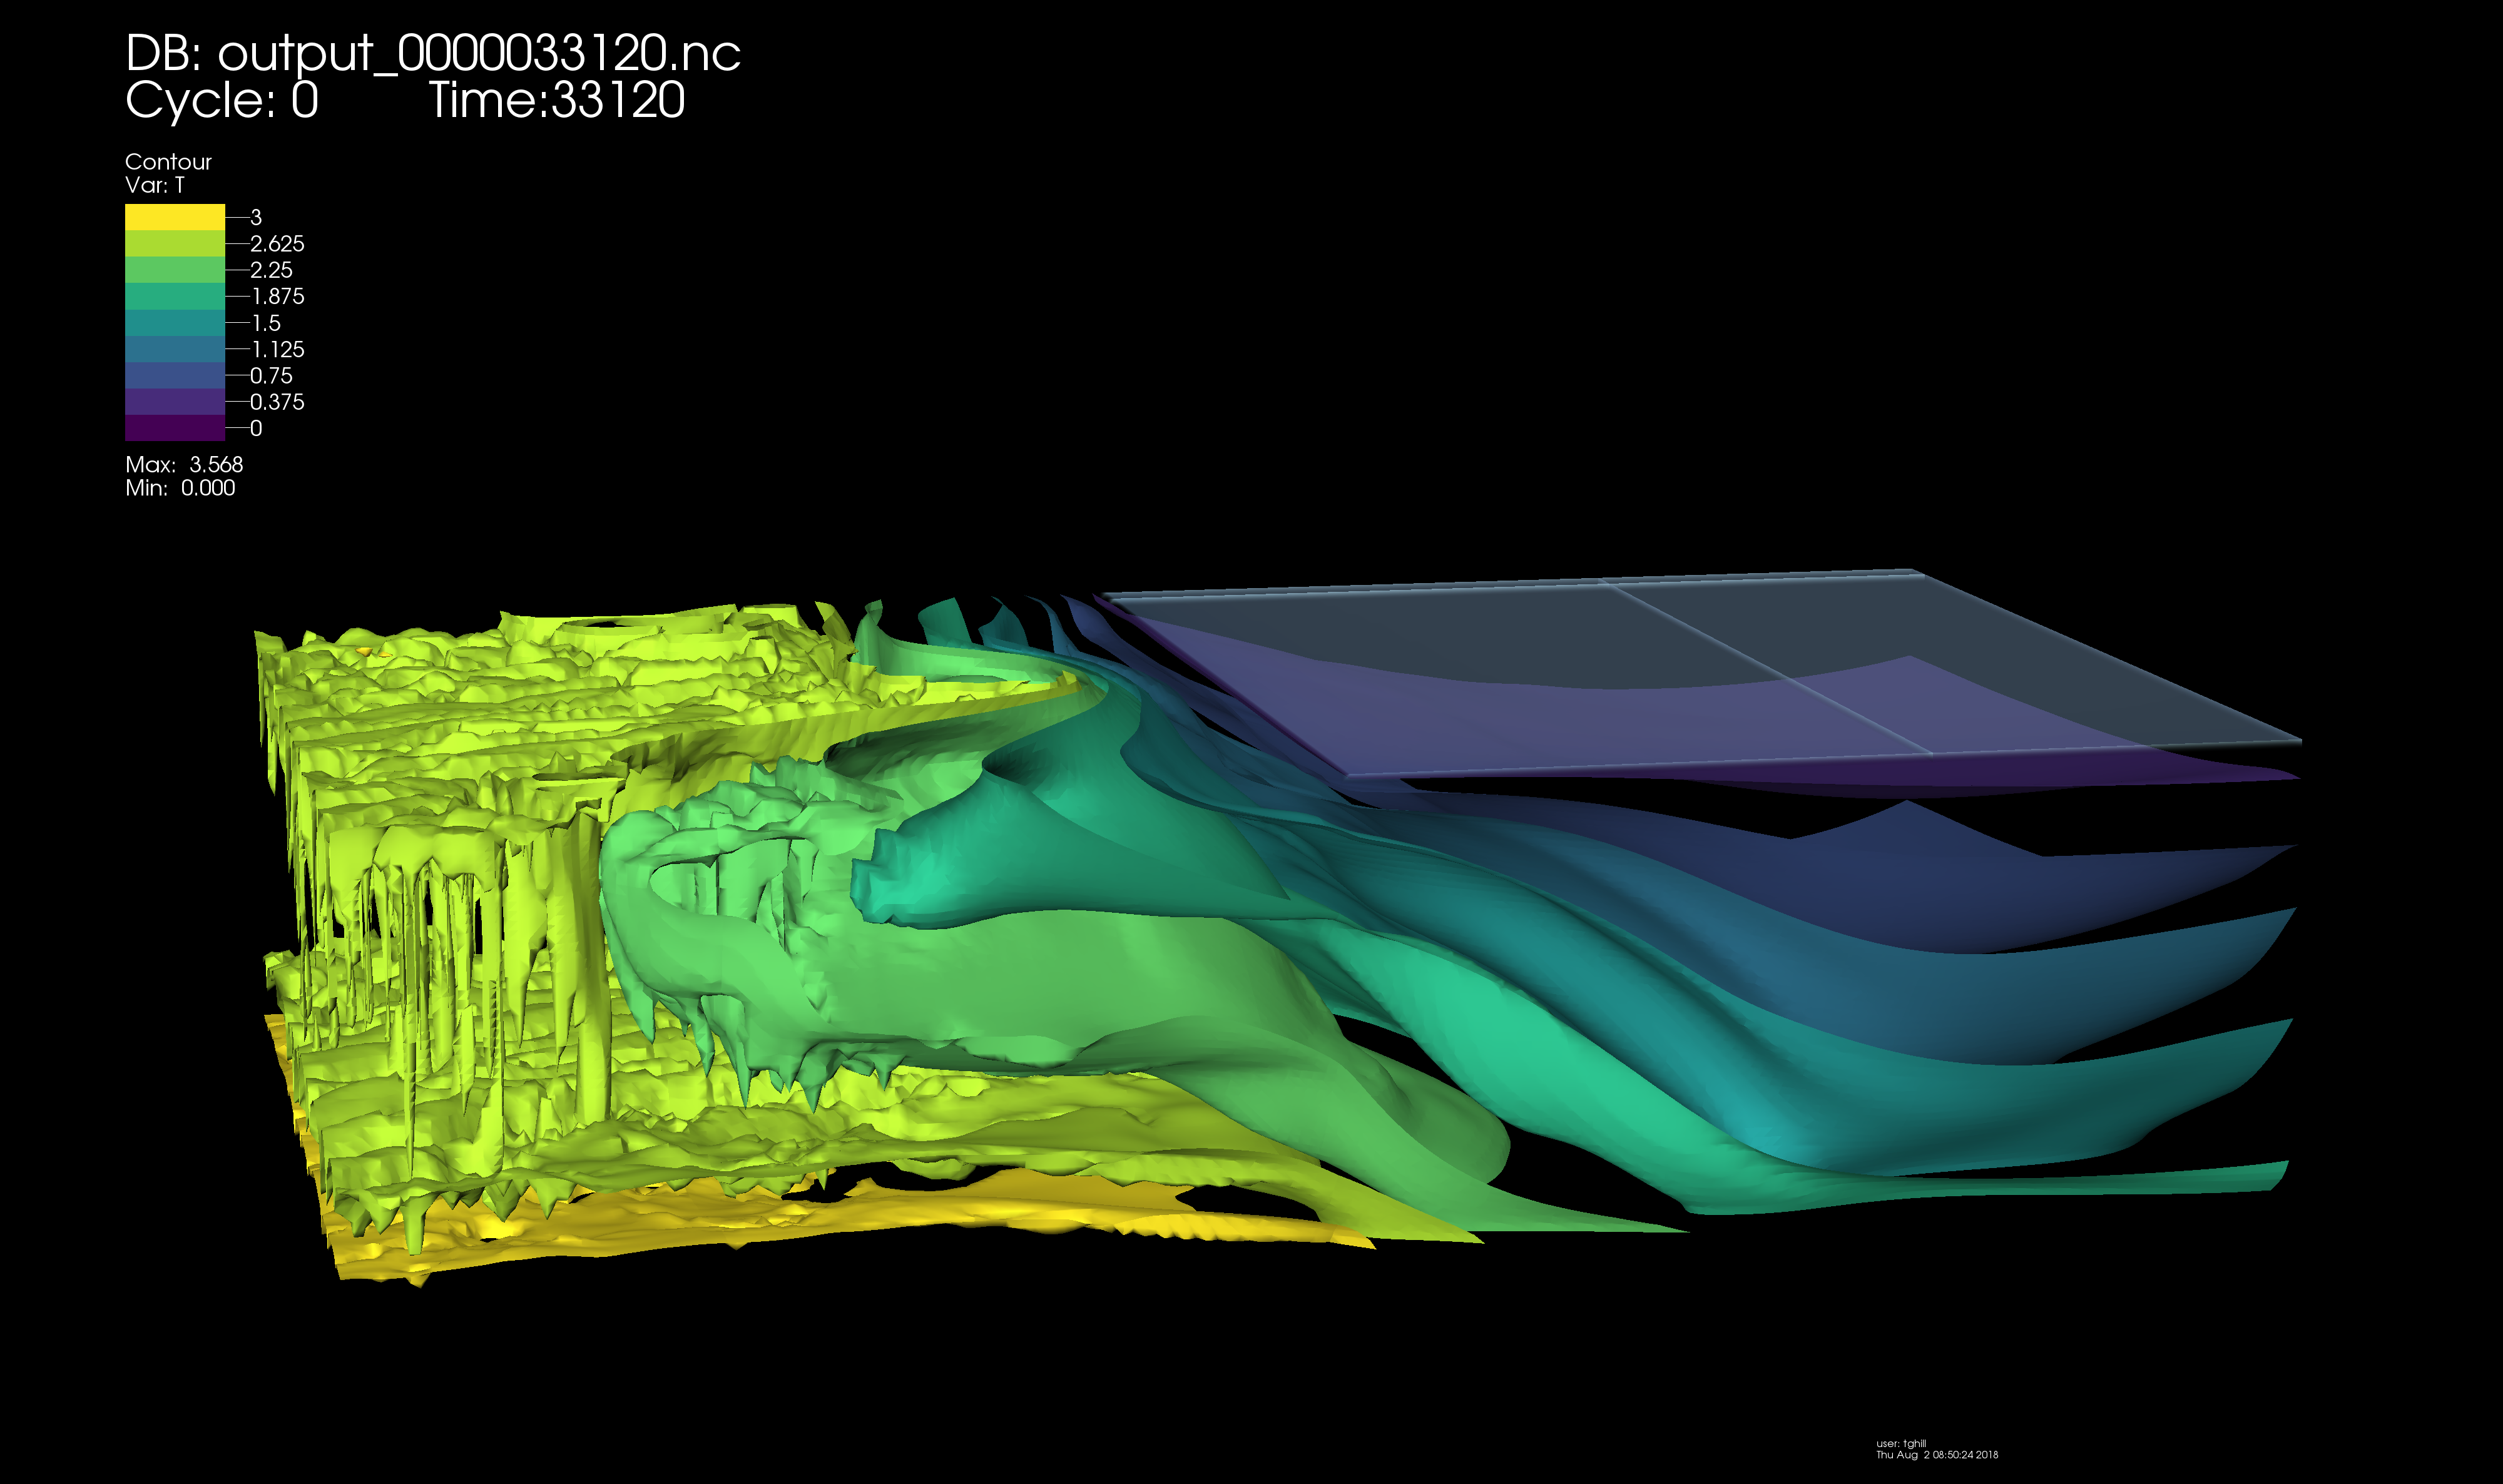
\includegraphics[width=\linewidth]{solarForcing/solarforcing-section02}
\end{subfigure}
\caption{Constant temperature surfaces for hydrostatic configuration of case 3. The top panel shows the entire domain. The bottom panels show two perspectives of a cut of the east half of the domain. The forward face in the bottom left is the center of the domain. The forward face in the bottom right is the Eastern edge of the domain.}
\label{fig:solarForcingConstantT}
\end{figure}

This case was also run in non-hydrostatic configuration. A comparison of the kinetic energy, internal energy, and ice mass are shown in figure \ref{fig:solarForcingCompare}. The kinetic energies agree very well, and the internal energy and ice mass are even closer. This might not be the case for higher resolutions, but this was not studied. This case has a horizontal resolution of $\SI{20}{m}$ and a vertical resolution of $\SI{20}{cm}$. If the resolution is increased to closer to $\SI{5}{m}$ as in the ice melting high resolution cases the curves might diverge.

\clearpage
\begin{figure}[h!]
\centering
\begin{subfigure}{0.98\linewidth}
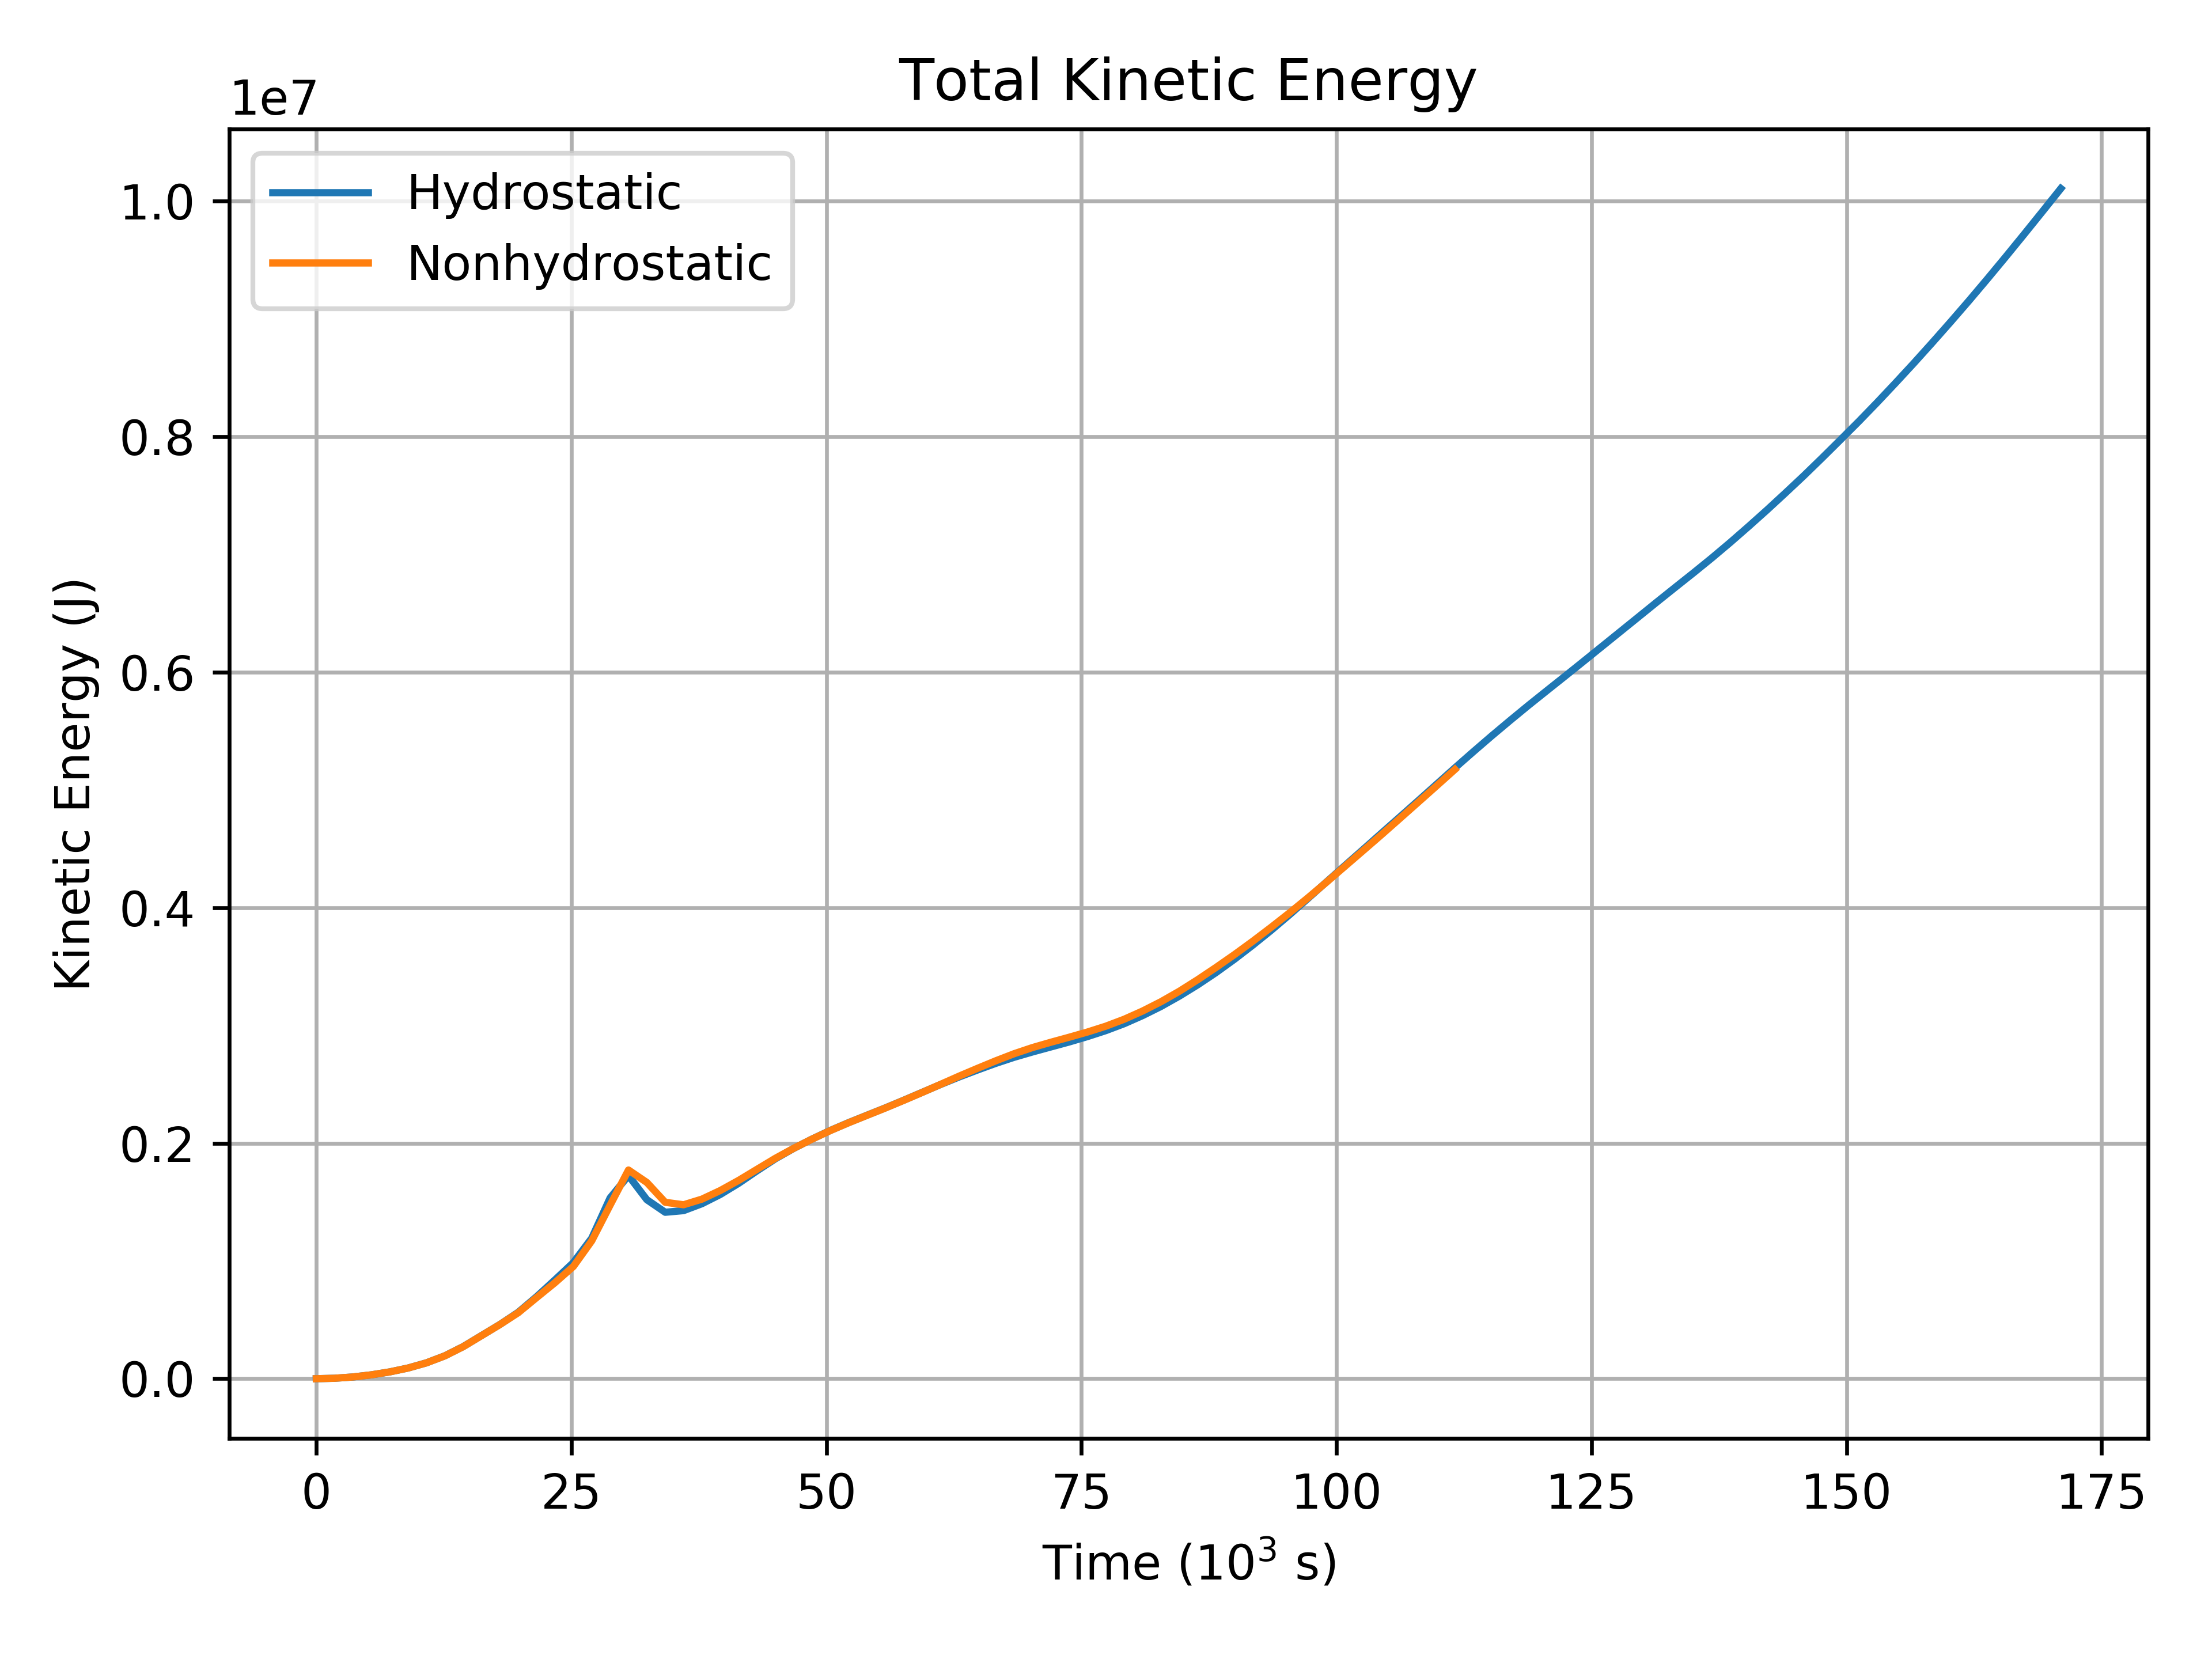
\includegraphics[width=\linewidth]{solarForcing/convect-deltaTKE}
\end{subfigure}

\begin{subfigure}{0.49\linewidth}
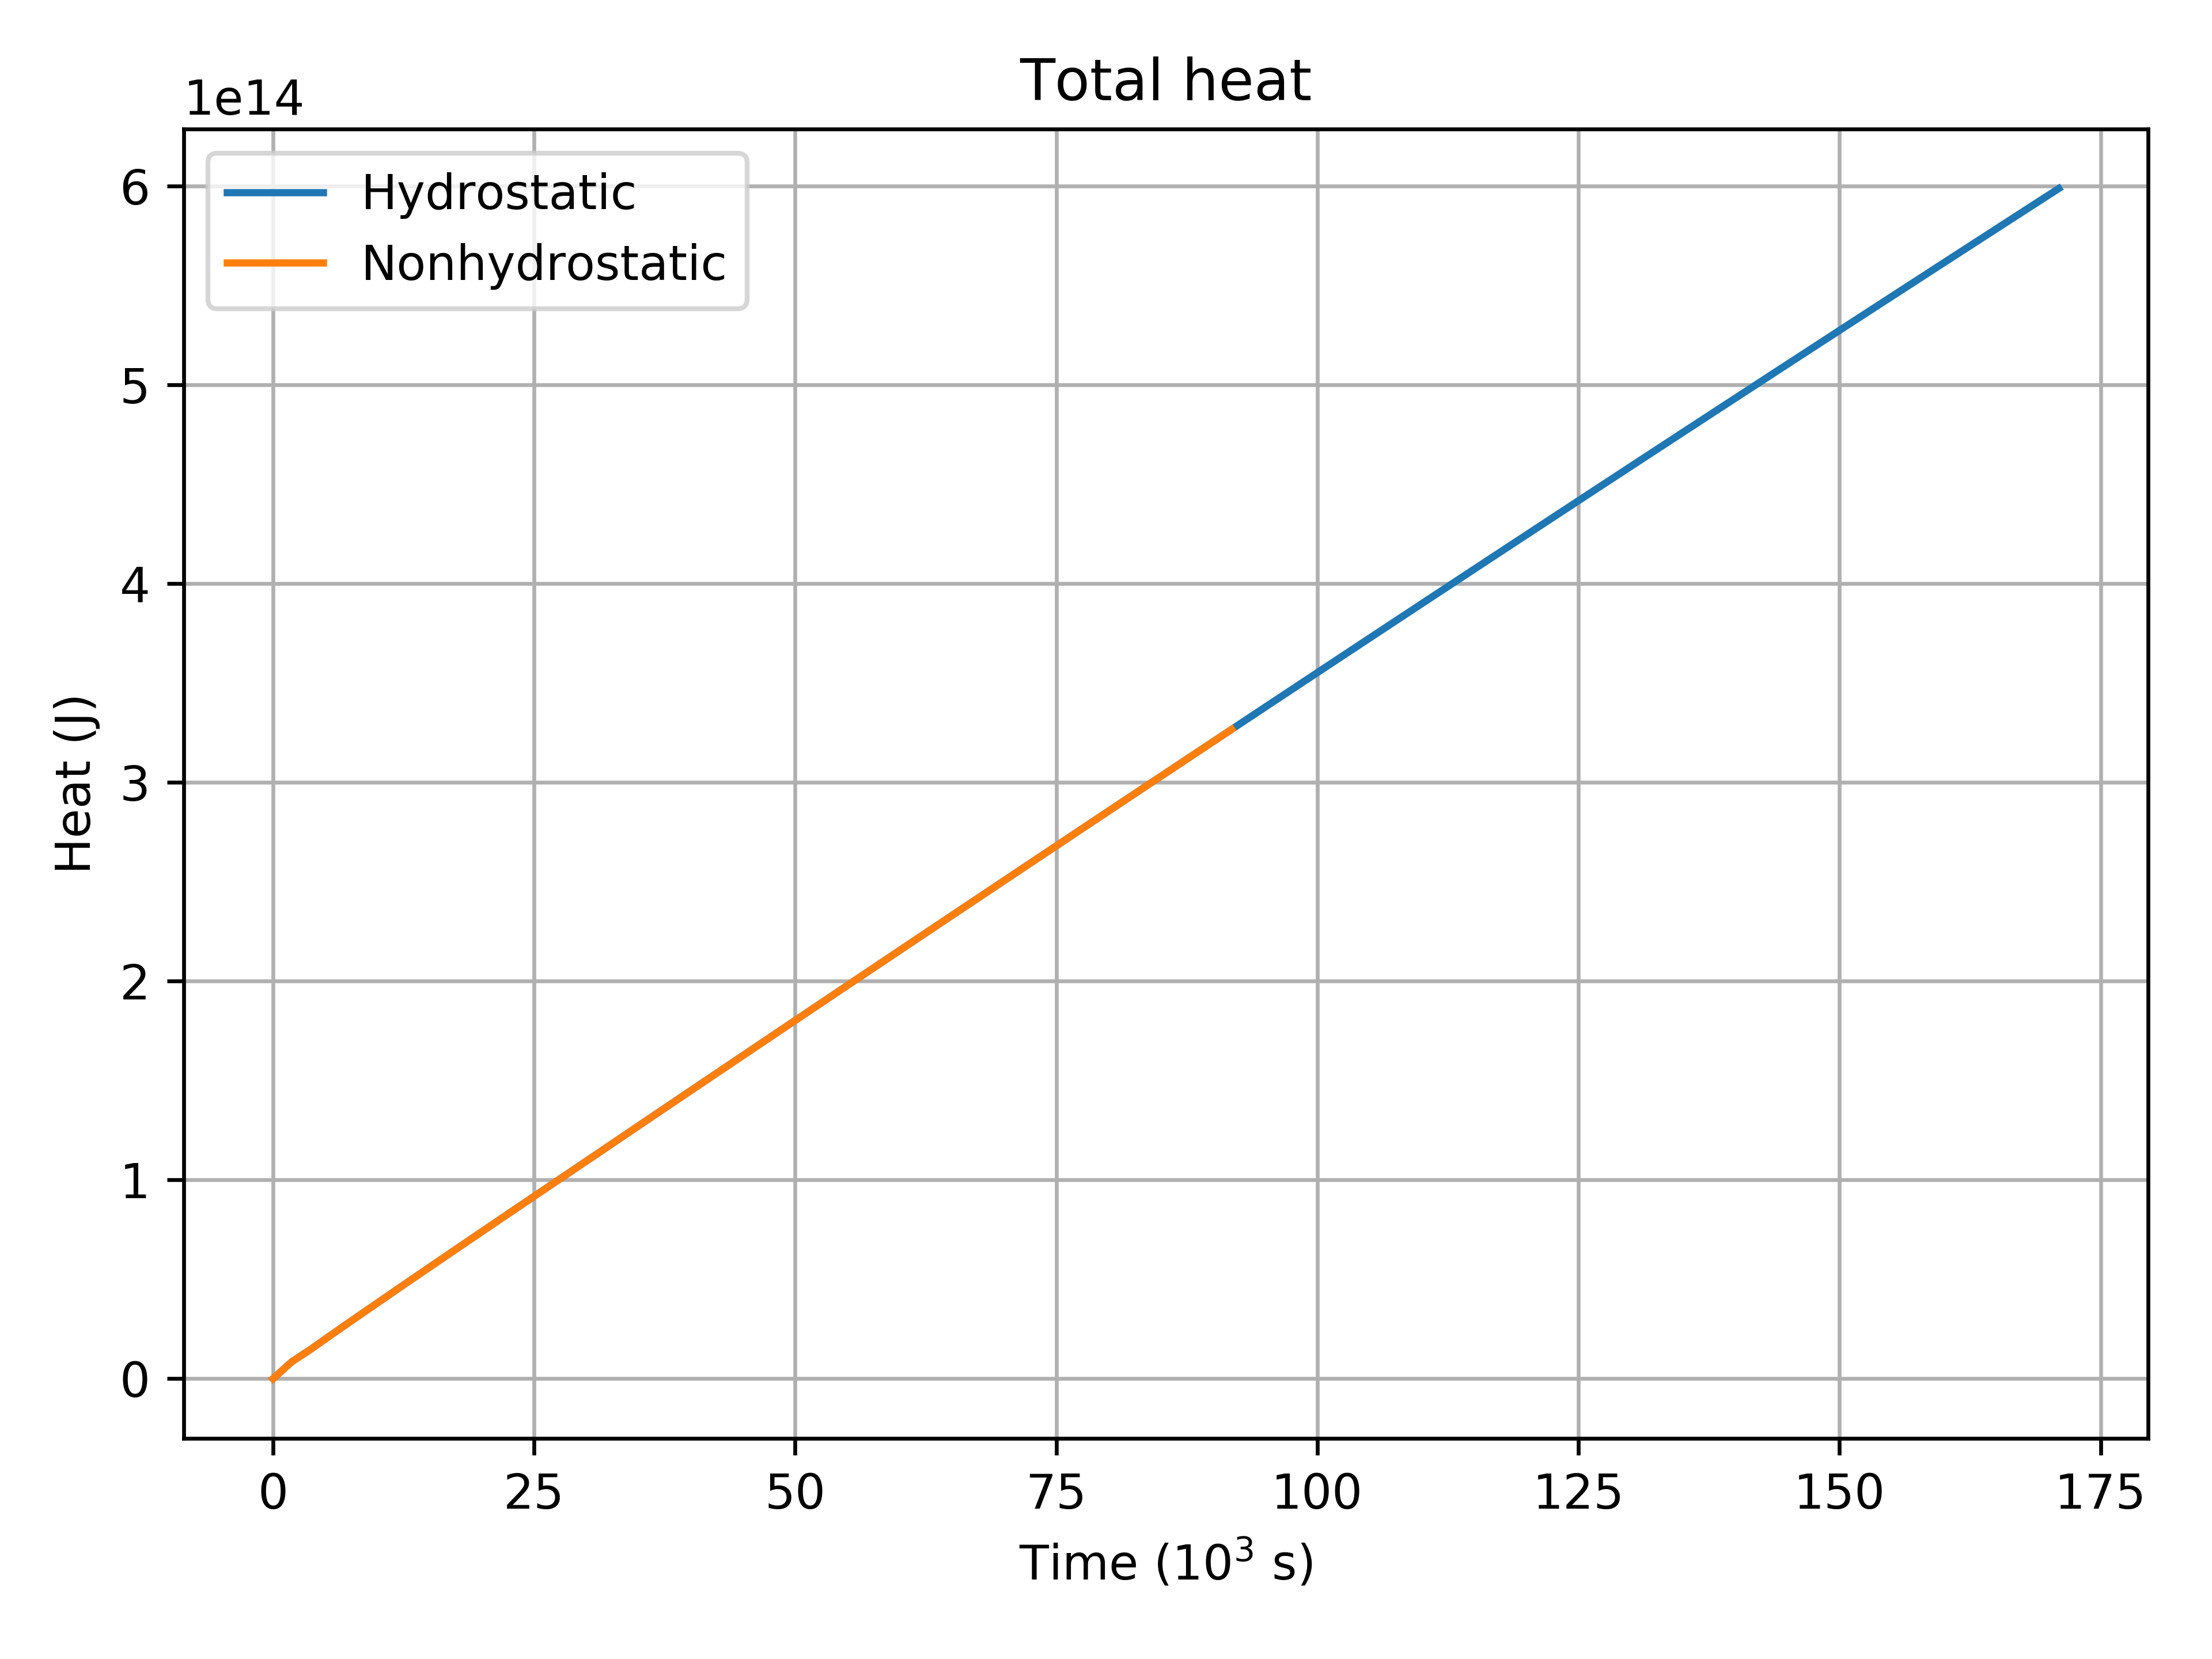
\includegraphics[width=\linewidth]{solarForcing/convect-deltaQ}
\end{subfigure}
\begin{subfigure}{0.49\linewidth}
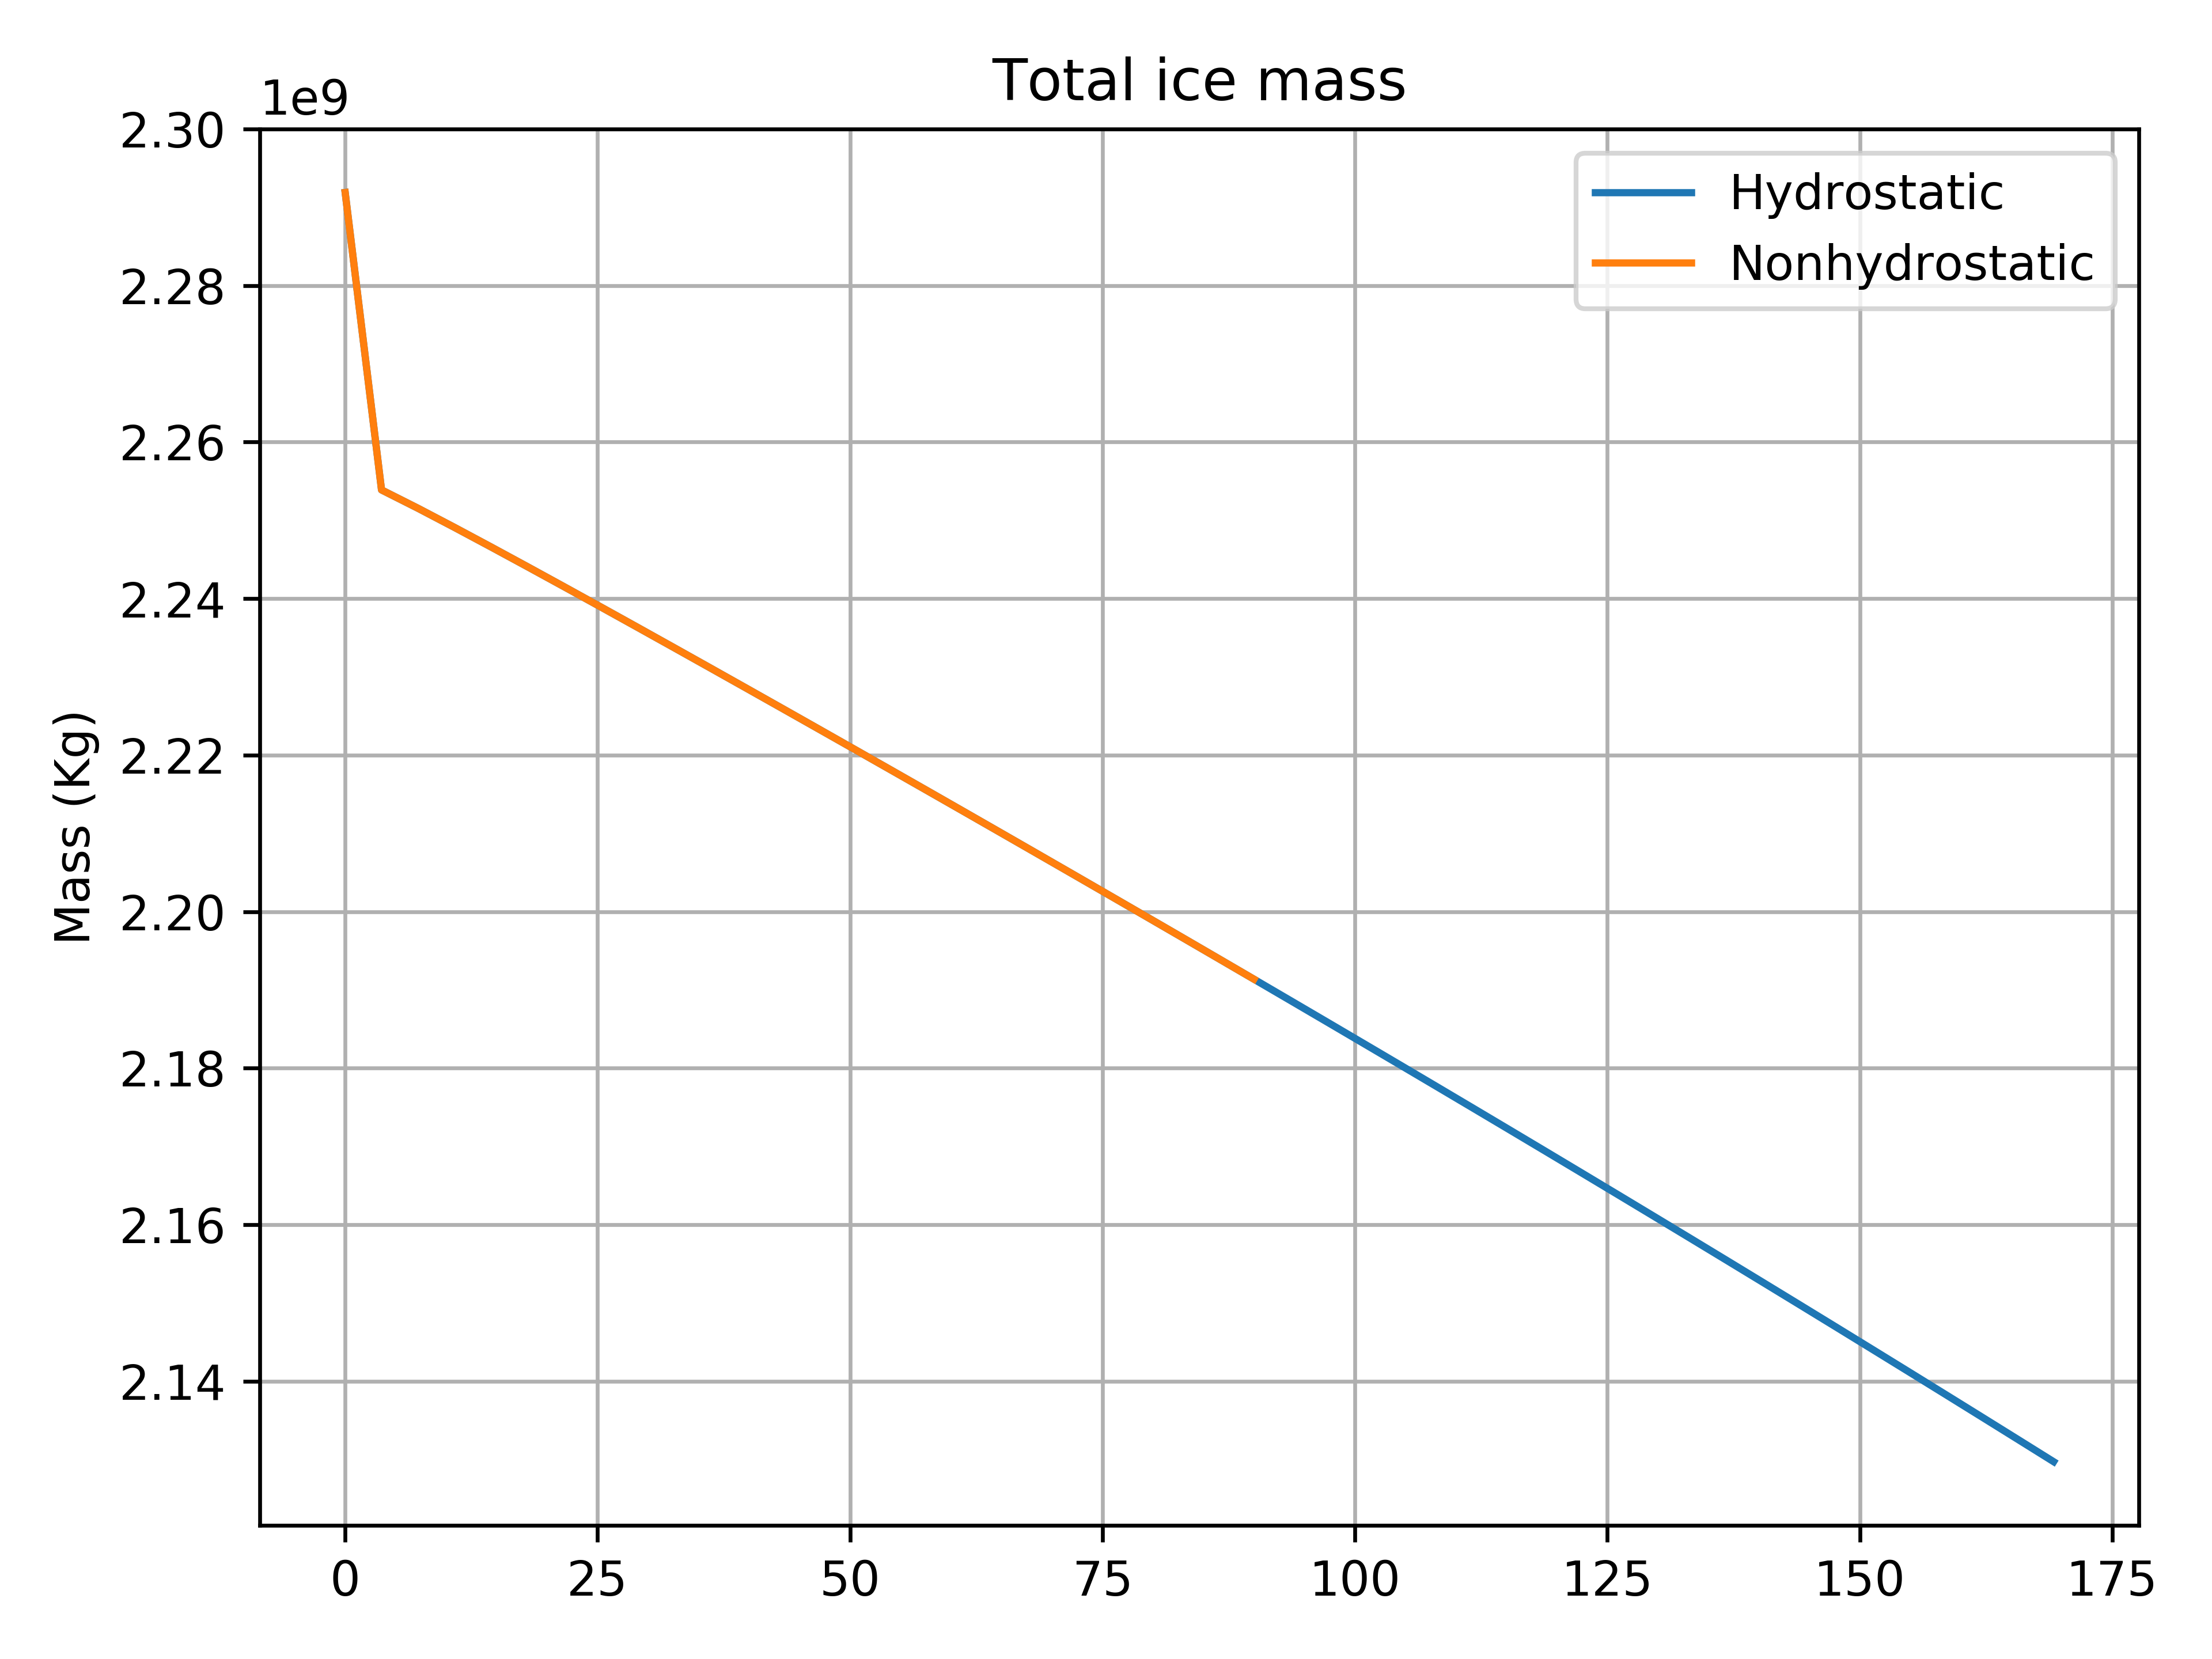
\includegraphics[width=\linewidth]{solarForcing/convect-deltaIce}
\end{subfigure}
\caption{Case 3: comparison of total kinetic energy (top), internal energy in the water (bottom left) and ice mass (bottom right) for hydrostatic and non-hydrostatic configurations.}
\label{fig:solarForcingCompare}
\end{figure}

\subsubsection{What was learned}
From this case, we see that the treatment of solar radiation is consistent with our intuition. At the resolution used, the difference between hydrostatic and non-hydrostatic configurations is very small. This was also a good test case for 3D visualization techniques (figure \ref{fig:solarForcingConstantT}).

\subsubsection{Next steps}
It might be worthwhile to run this case at higher resolution on Graham to see if the non-hydrostatic configuration has more kinetic energy from convection than the hydrostatic case. It would also be interesting to try to resolve the convection currents better and really study how they interact with the ice. This might require scaling the domain down to have much finer resolution.

\subsection{Case 4: Periodic forcing}
So far, all cases have used a similar domain, and have had constant forcing. We try running the model with a much larger domain and daily cycles in the forcing fields. We use a sinusoidal cycle as a rough approximation of the daily cycle of meteorological forcing (see figure \ref{fig:periodicForcingFields}).

The domain is a 25 km x 25 km square lake, modelled at 250 m resolution. The lake is 50 m deep, with 2 m vertical resolution. The sides of the lake are sloped with a constant 2\% slope (drops 50 m over 2.5 km). The meteorological forcing is shown in figure \ref{fig:periodicForcingFields}. Some more parameter details are given in table \ref{table:periodicForcing}.


\begin{longtable}{  p{.30\textwidth}  p{.30\textwidth}  p{.4\textwidth}  }
\hline
\textbf{Paramter Name} & \textbf{Parameter Value} & \textbf{Comment} \\ \hline \hline
\verb|Nx| & 100 & 25 x 4 processors \\ \hline
\verb|Ny| & 100 & 25 x 4 processors \\ \hline
\verb|tempAdvScheme|	&	33	&	High order advection scheme \\ \hline
\verb|nonHydrostatic| & \verb|.FALSE.| & Non-hydrostatic model configuration \\ \hline
\verb|eosType|		&	JMD95z	&	Polynomial approximation to true equation of state. This EOS respects the max in density at $4^{\circ} \textrm{C}$\\ \hline
\verb|delX|			&	\verb|100*250.0|	&	25 km lake, 250 m resolution \\ \hline
\verb|delY|			&	\verb|100*250.0|	&	25 km lake, 250 m resolution \\ \hline
\verb|delZ|			&	\verb|25*2.0|	&	50 m deep lake, 2 m resolution \\ \hline

\verb|uwind|		&	Sinusoidal between $\pm \SI{1}{m/s}$ & Daily cycle with average of $0$  \\ \hline
\verb|vwind| 	& 0	& \\ \hline
\verb|atemp| 	& Sinusoidal between $-5$ and $\SI{15}{\celsius}$ & Daily cycle with average of $+\SI{5}{\celsius}$ \\ \hline
\verb|aqh| 		& $0.01$		&	Specific humidity \\ \hline
\verb|swdown| 	& Sinusoidal between $0$ and $\SI{500}{W.m^{-2}}$	& Daily cycle of SW radiation \\ \hline
\verb|lwdown| 	& Sinusoidal between $50$ and $\SI{550}{W.m^{-2}}$	& Daily cycle of LW radiation, respect minimum LW radiation \\ \hline

\verb|SEAICEuseDYNAMICS| & \verb|.TRUE.| & Allow SEAICE dynamics \\ \hline
\verb|SEAICE_area_reg|   & \verb|1.0E-5| & Ice fraction less than this will be treated as zero ice for next time step \\ \hline
\verb|SEAICE_hice_reg|   & \verb|1.0E-5| & Height cutoff \\ \hline
\verb|SEAICEadvHEFF|     & \verb|.TRUE.| & Advect effective height \\ \hline
\verb|SEAICEadvAREA|     & \verb|.TRUE.| & Advect seaice area fraction \\ \hline
\verb|SEAICEadvScheme|   & 33			& Advection scheme 33: Flux limited direct space and time advection scheme \\ \hline

Temperature & \begin{equation*} \begin{cases} 0^{\circ} \text{C} & z = 0 \text{ m} \\ 4 ^{\circ} \text{C} & z = -50 \text{ m}   \end{cases} \end{equation*} & Temperature stratified lake, pycnocline at $\SI{25}{m}$, mid-depth \\ \hline
Initial SEAICE area fraction   & Large chunks, $0.2 \leq \texttt{SIarea} \leq 1.0$ & Variable ice cover \\ \hline
Initial SEAICE thickness    & Large chunks, $0.5 \leq \texttt{SIheff} \leq 1.0$ & Variable ice cover \\ \hline

\caption{Parameter values for case 3: solar forcing}
\label{table:periodicForcing}
\end{longtable}

\begin{figure}[h!]
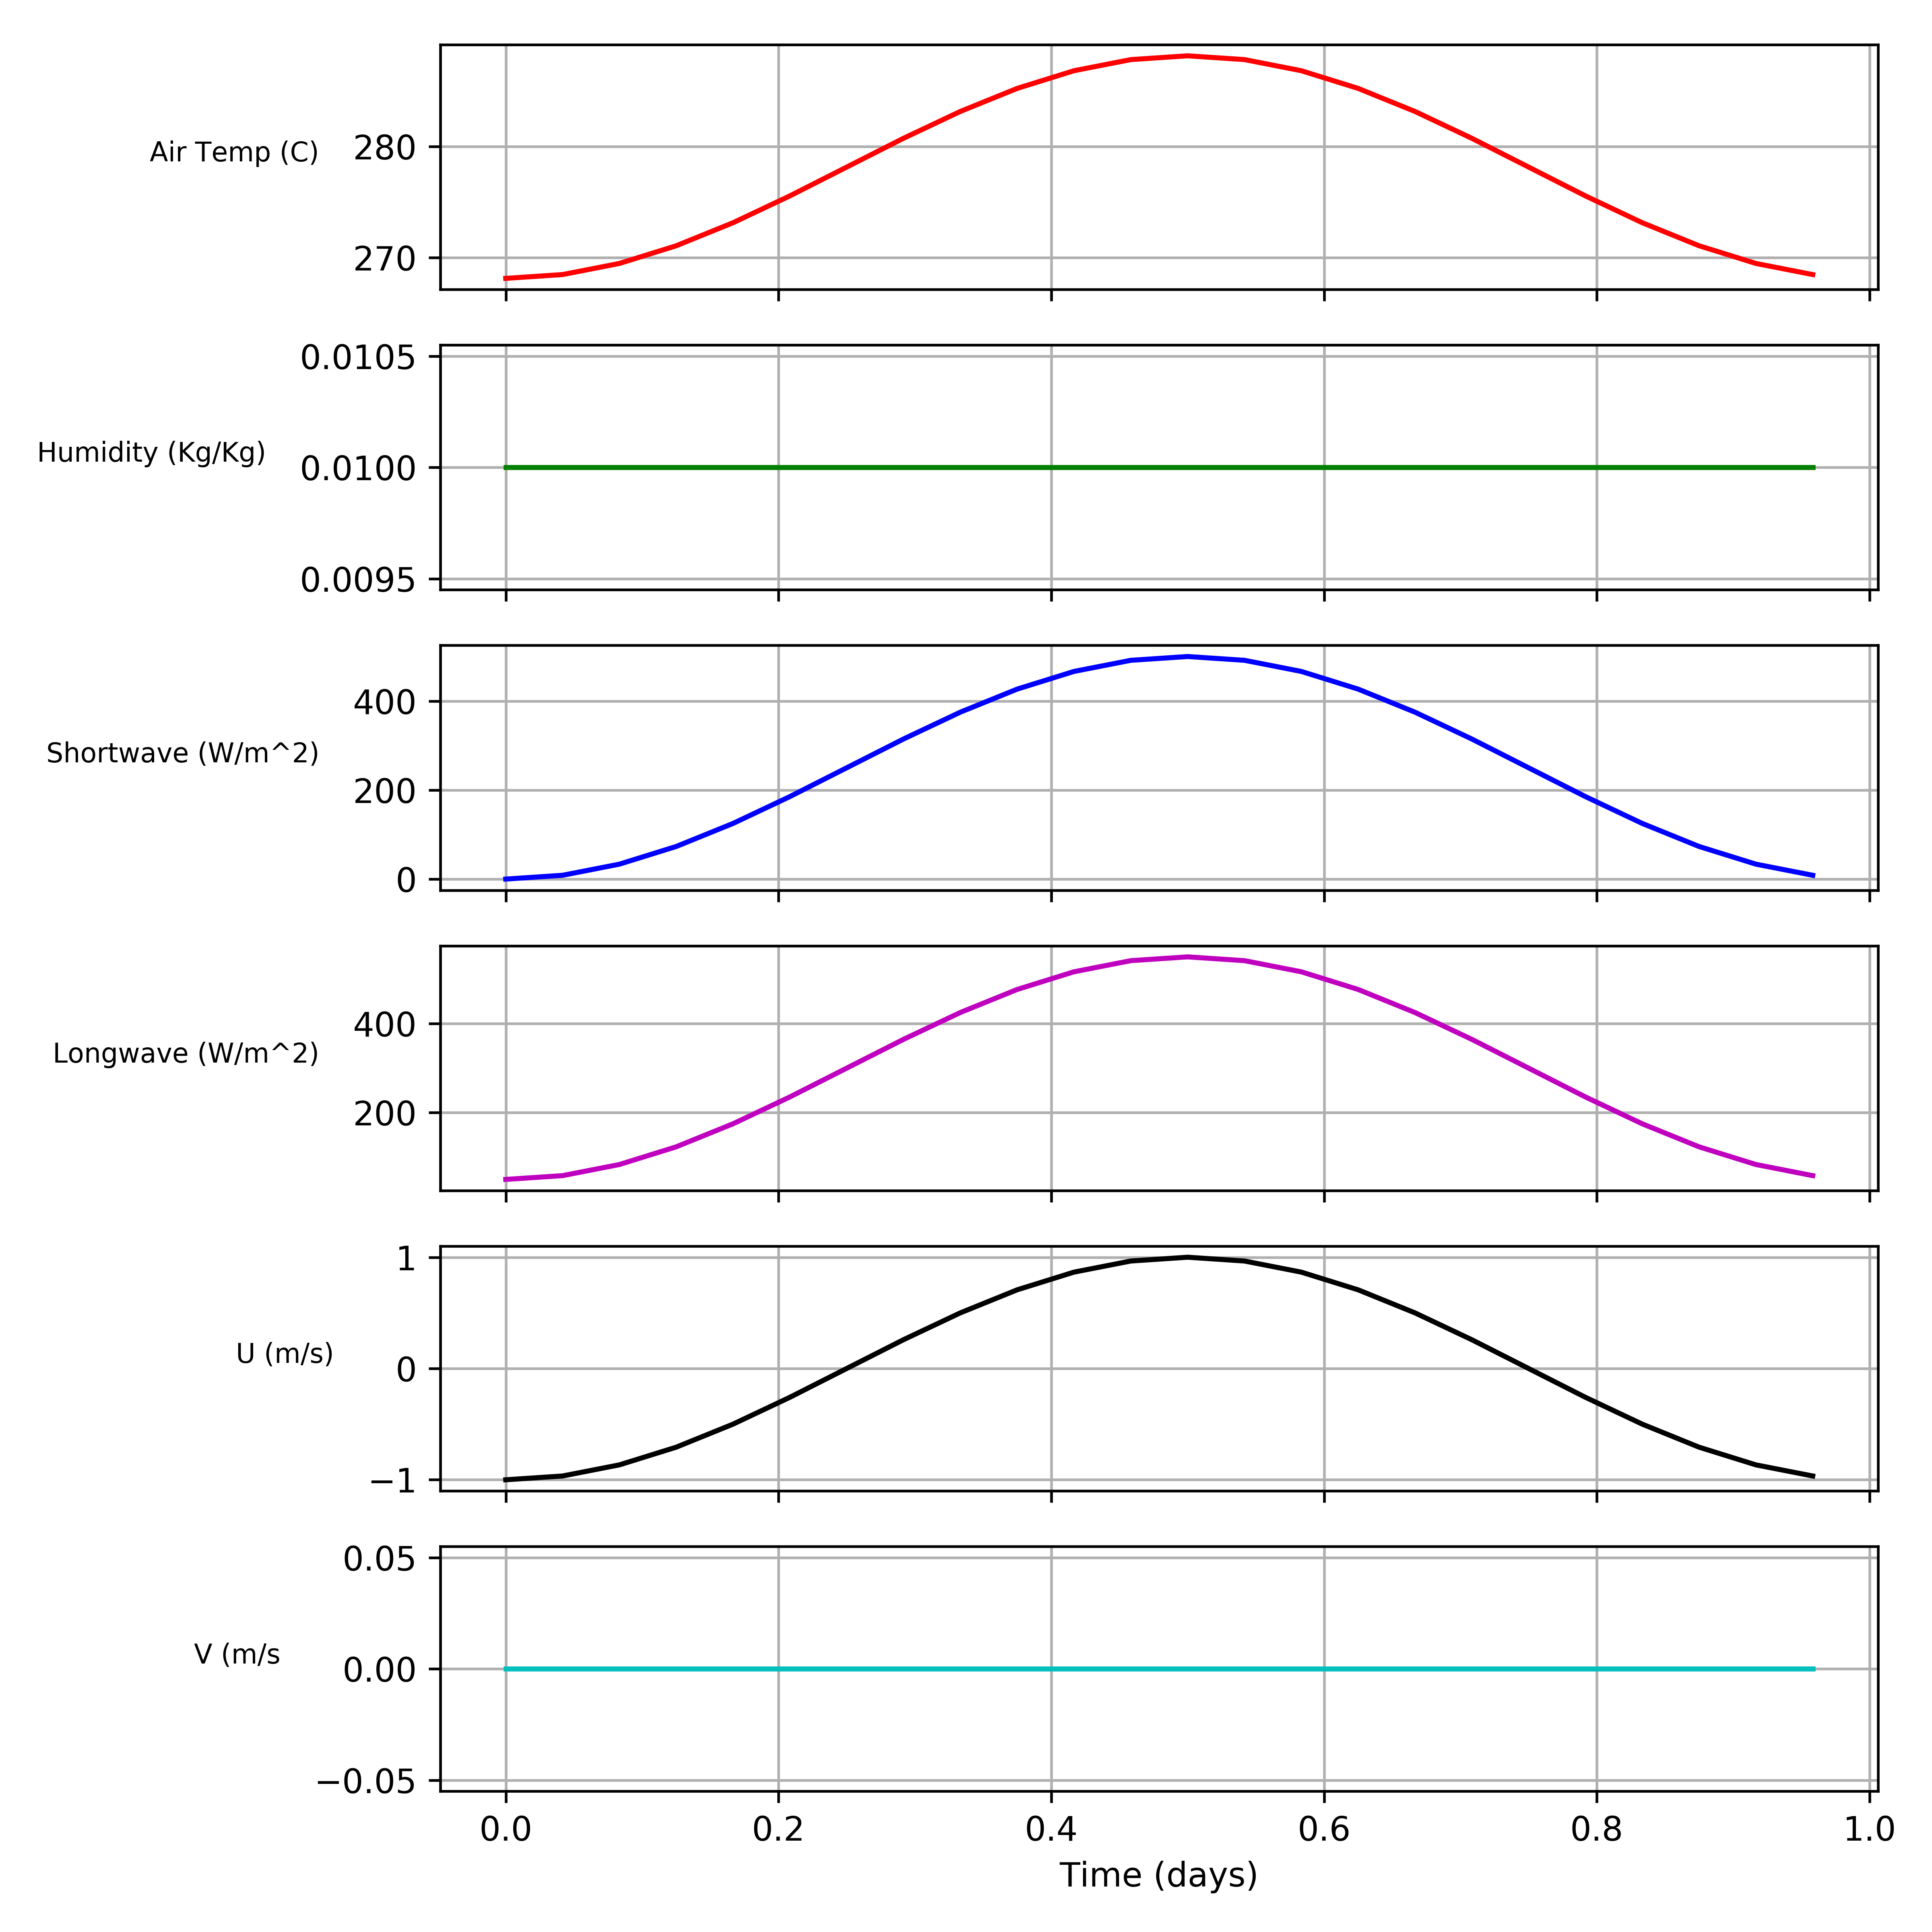
\includegraphics[width=\linewidth]{periodicForcing/forcing}
\caption{Time-dependent forcing values for case 4. Fields are sampled every hour (same frequency as output files are generated).}
\label{fig:periodicForcingFields}
\end{figure}

\subsubsection{Results}
\begin{figure}[h!]
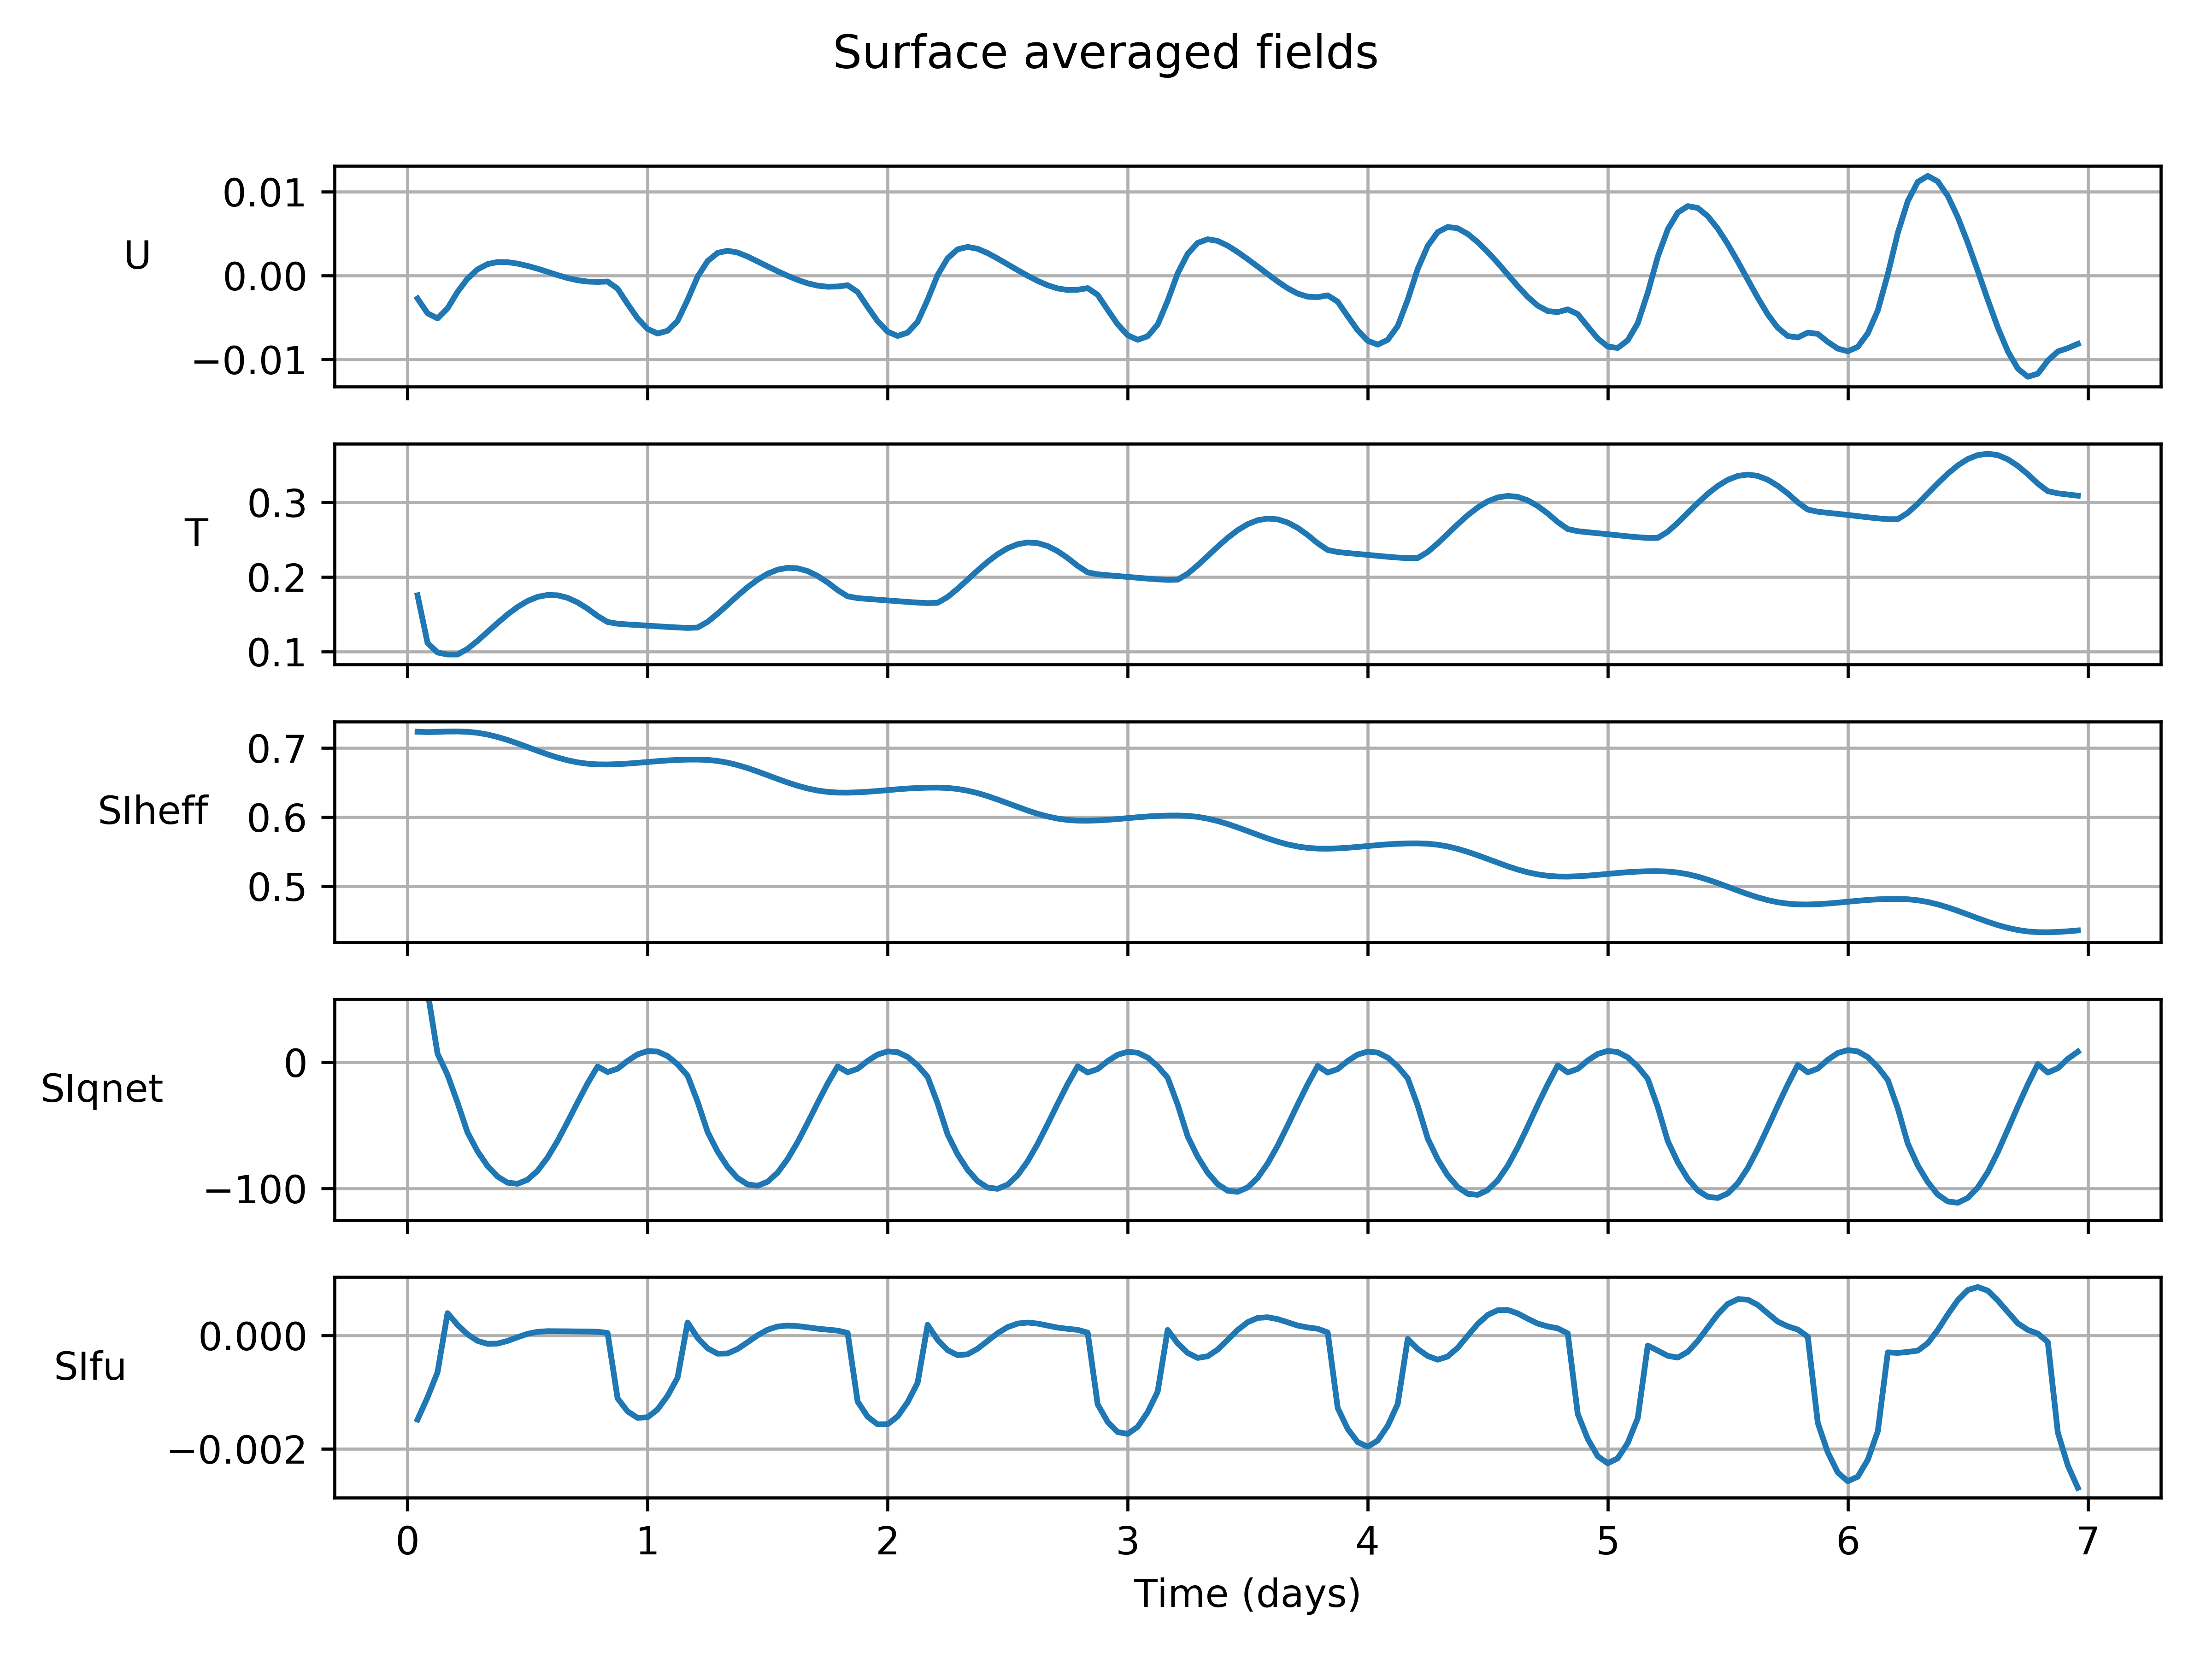
\includegraphics[width=\linewidth]{periodicForcing/response-fields}
\caption{Mean value of output fields in response to periodic forcing for case 4. From top to bottom: mean surface U currents, mean surface temperature, mean effective ice thickness, mean heat transfer from the lake into the ice, mean surface wind stress (U direction)}
\label{fig:periodicForcingResponse}
\end{figure}

We expect a roughly sinusoidal signal in the output fields in response to the input forcing (fig \ref{fig:periodicForcingFields}). The mean value of the output fields is shown in figure \ref{fig:periodicForcingResponse}. Notice the strange shape of the wind stress curve, and that the peak positive $U$ value occurs before midday. We would expect the peak positive surface currents to occur at or slightly after the peak positive wind speed, but the currents appear to lead the wind.

A 3D visualization of this case is shown in figure \ref{fig:periodicVisualization}. This visualization is a cut of the north half of the domain, with the open face the center of the domain. You can see some variability in the upper constant T contours, created by the initial variability in the ice cover.

\begin{figure}[h!]
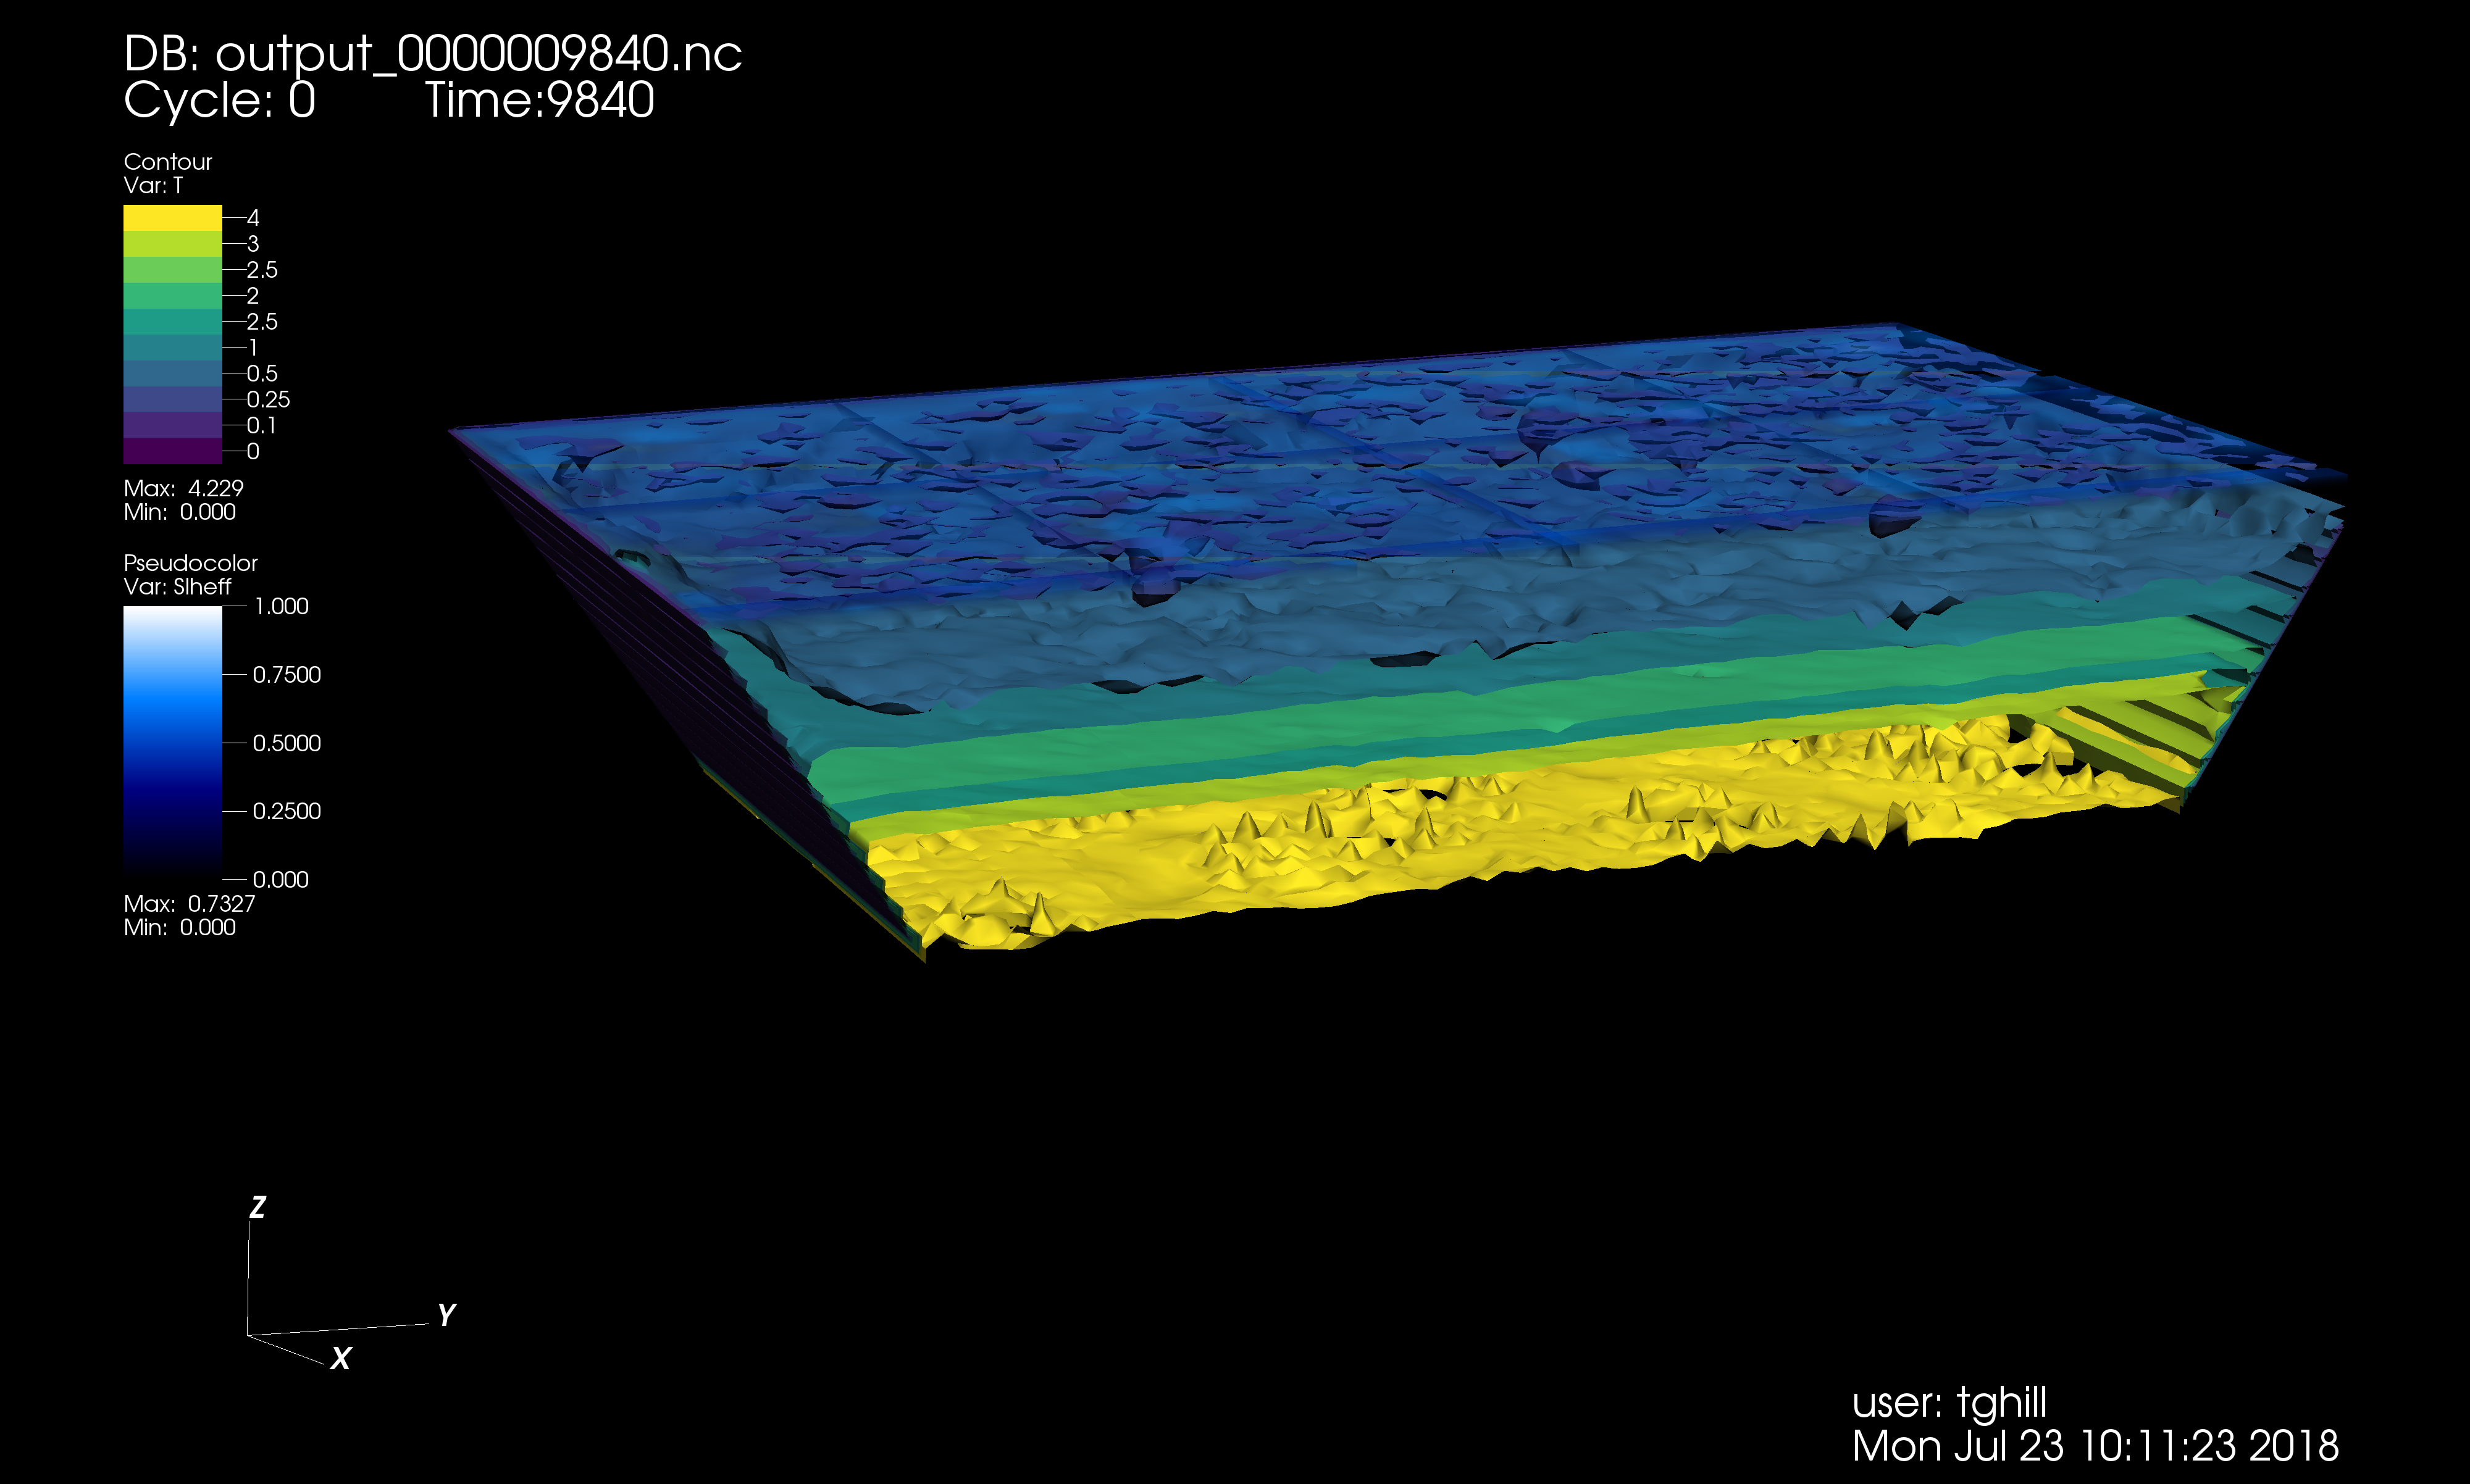
\includegraphics[width=\linewidth]{periodicForcing/domain-results}
\caption{3D visualization of the temperature and ice thickness for case 4 with periodic forcing.}
\label{fig:periodicVisualization}
\end{figure}

\subsubsection{Run with constant temperature}
We want to see what happens when we run this case with no temperature stratification. The response curves above have the strange "capped" structure, and we want to know if this goes away or stays when we take out the stratification. The capped structure could be due to the wind creating an internal seiche, and removing the stratification would remove the seiche. We set the initial water to constant $\SI{0}{\celsius}$.

Running this case, the response curves have the same shape (figure \ref{fig:periodicForcingResponseConstantT}).

This case NaN'd before the end of the model time (1 week). The other case did not NaN. I don't know why this case broke and the other didn't.

\begin{figure}[h!]
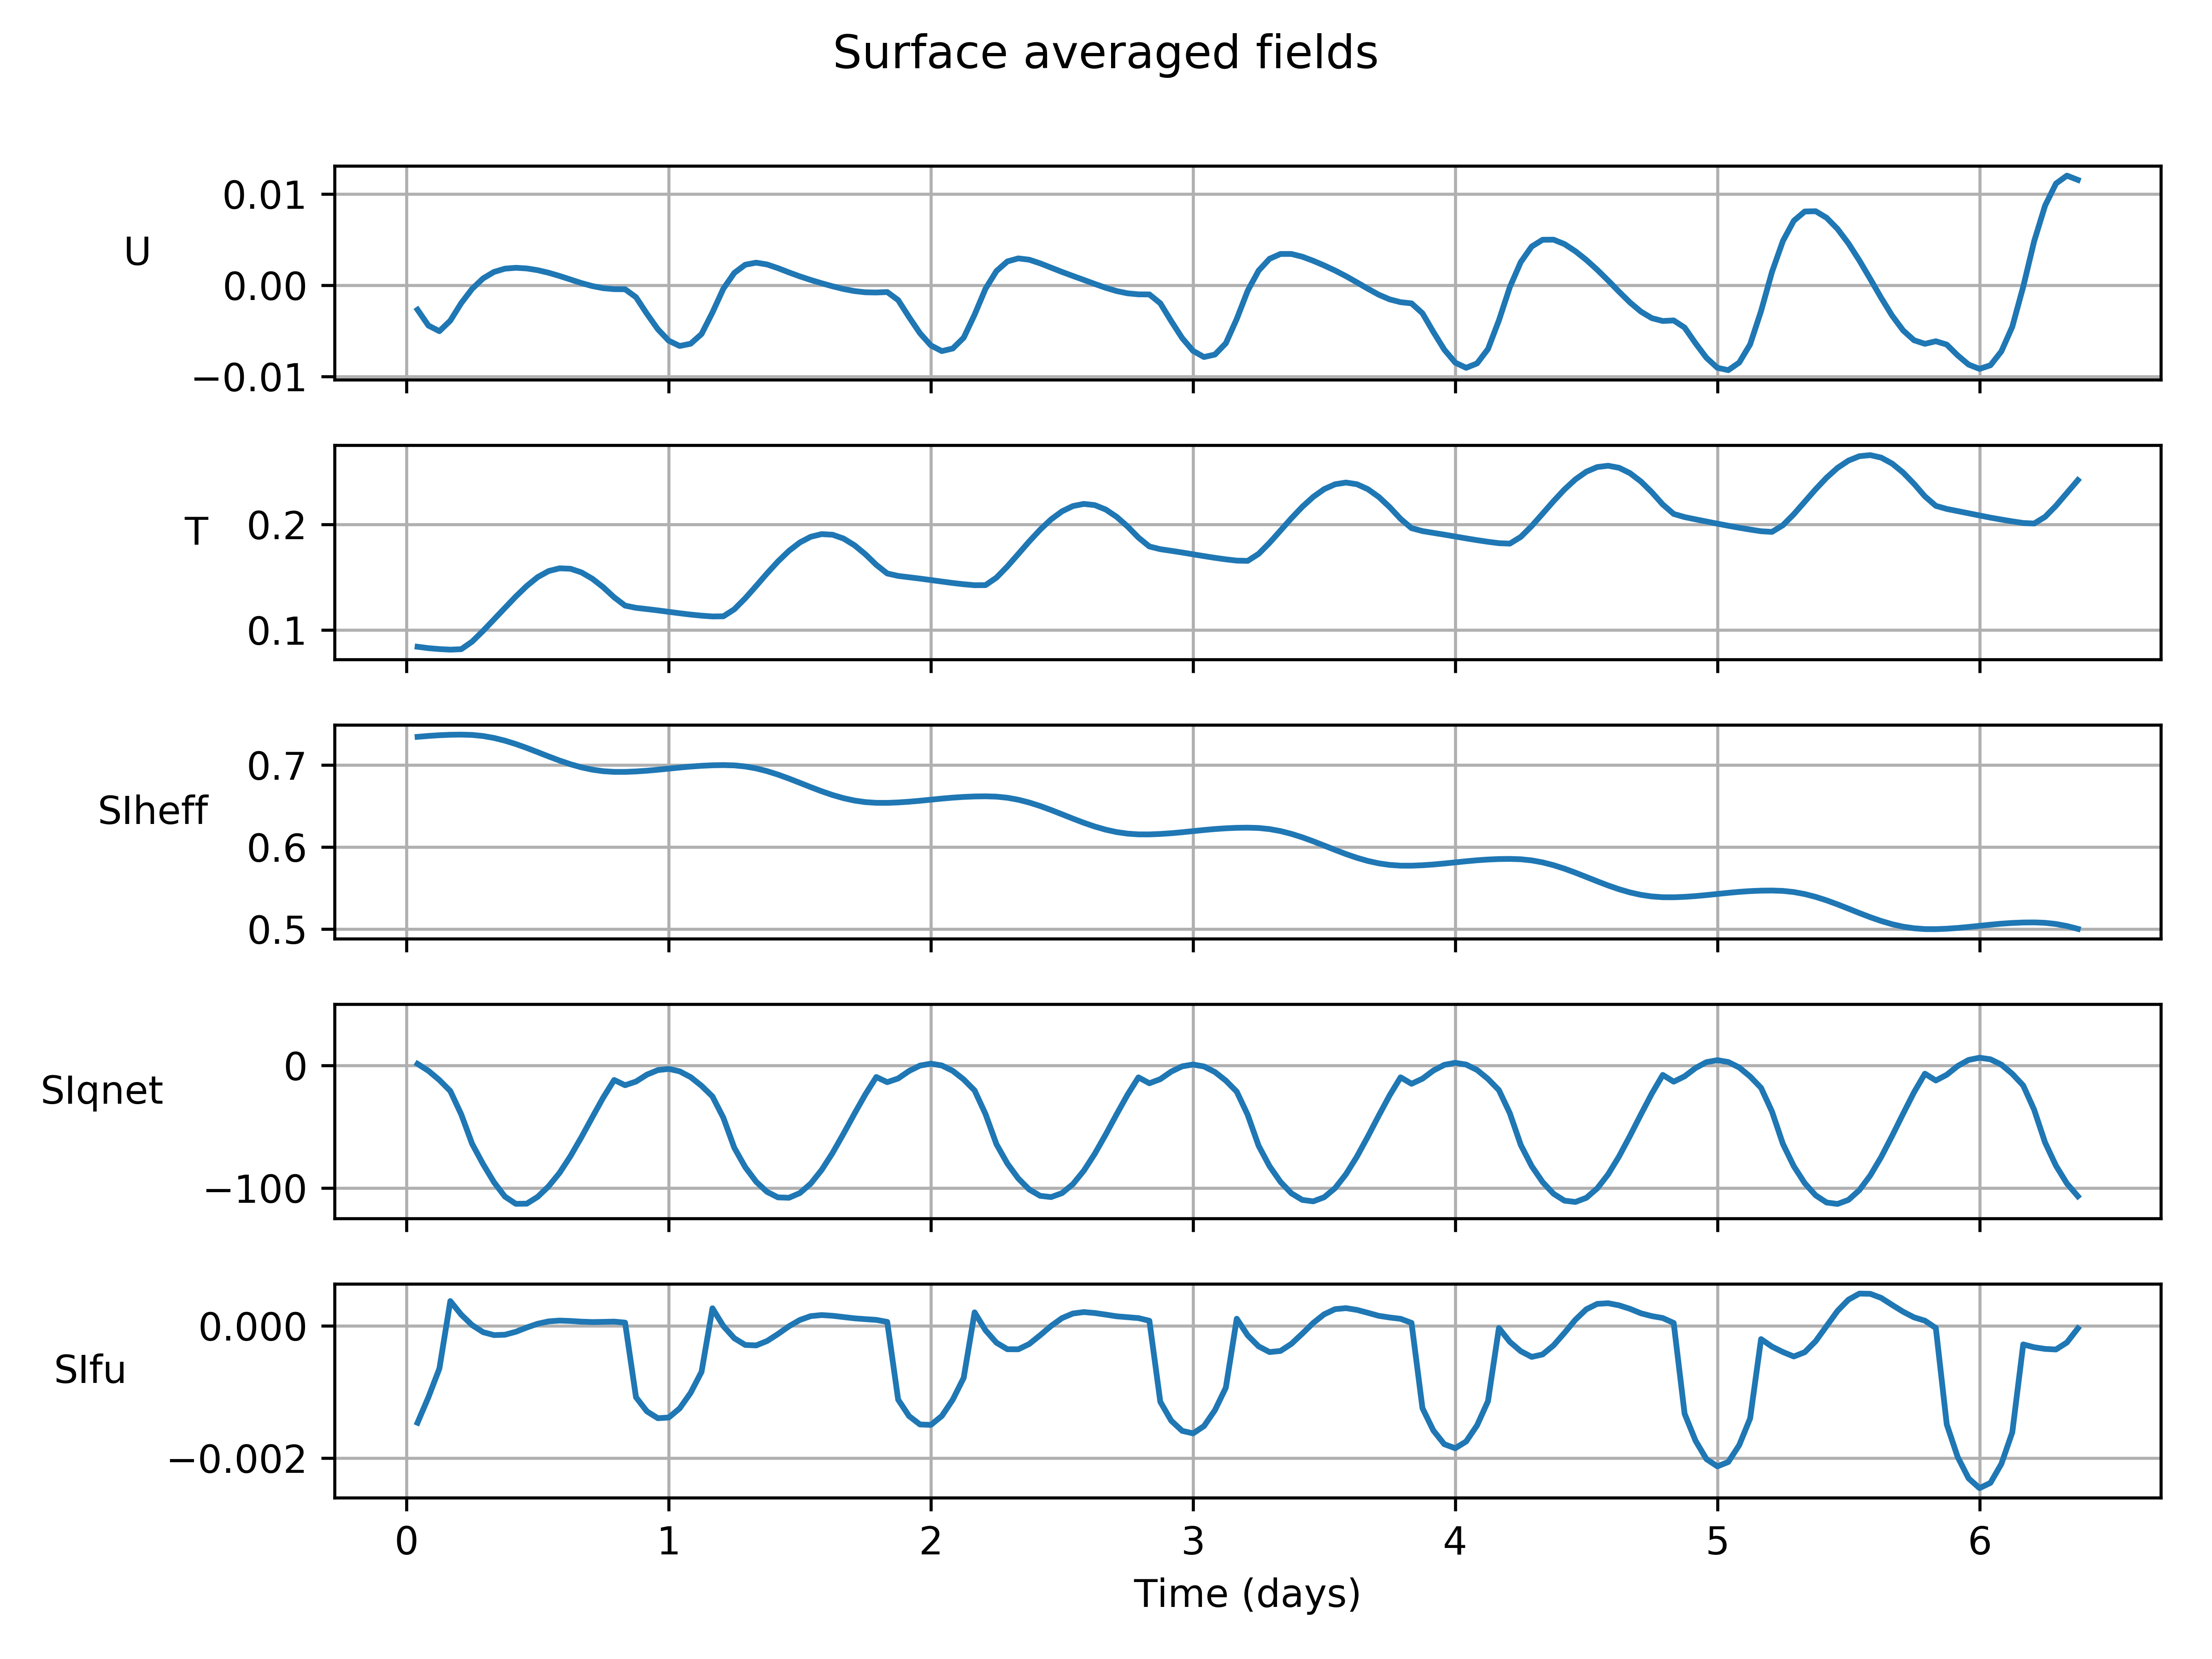
\includegraphics[width=\linewidth]{periodicForcing/response-constantT-fields}
\caption{Mean value of output fields in response to periodic forcing, with no temperature stratification. From top to bottom: mean surface U currents, mean surface temperature, mean effective ice thickness, mean heat transfer from the lake into the ice, mean surface wind stress (U direction)}
\label{fig:periodicForcingResponseConstantT}
\end{figure}

\begin{figure}[h!]
\centering
\begin{subfigure}{0.48\linewidth}
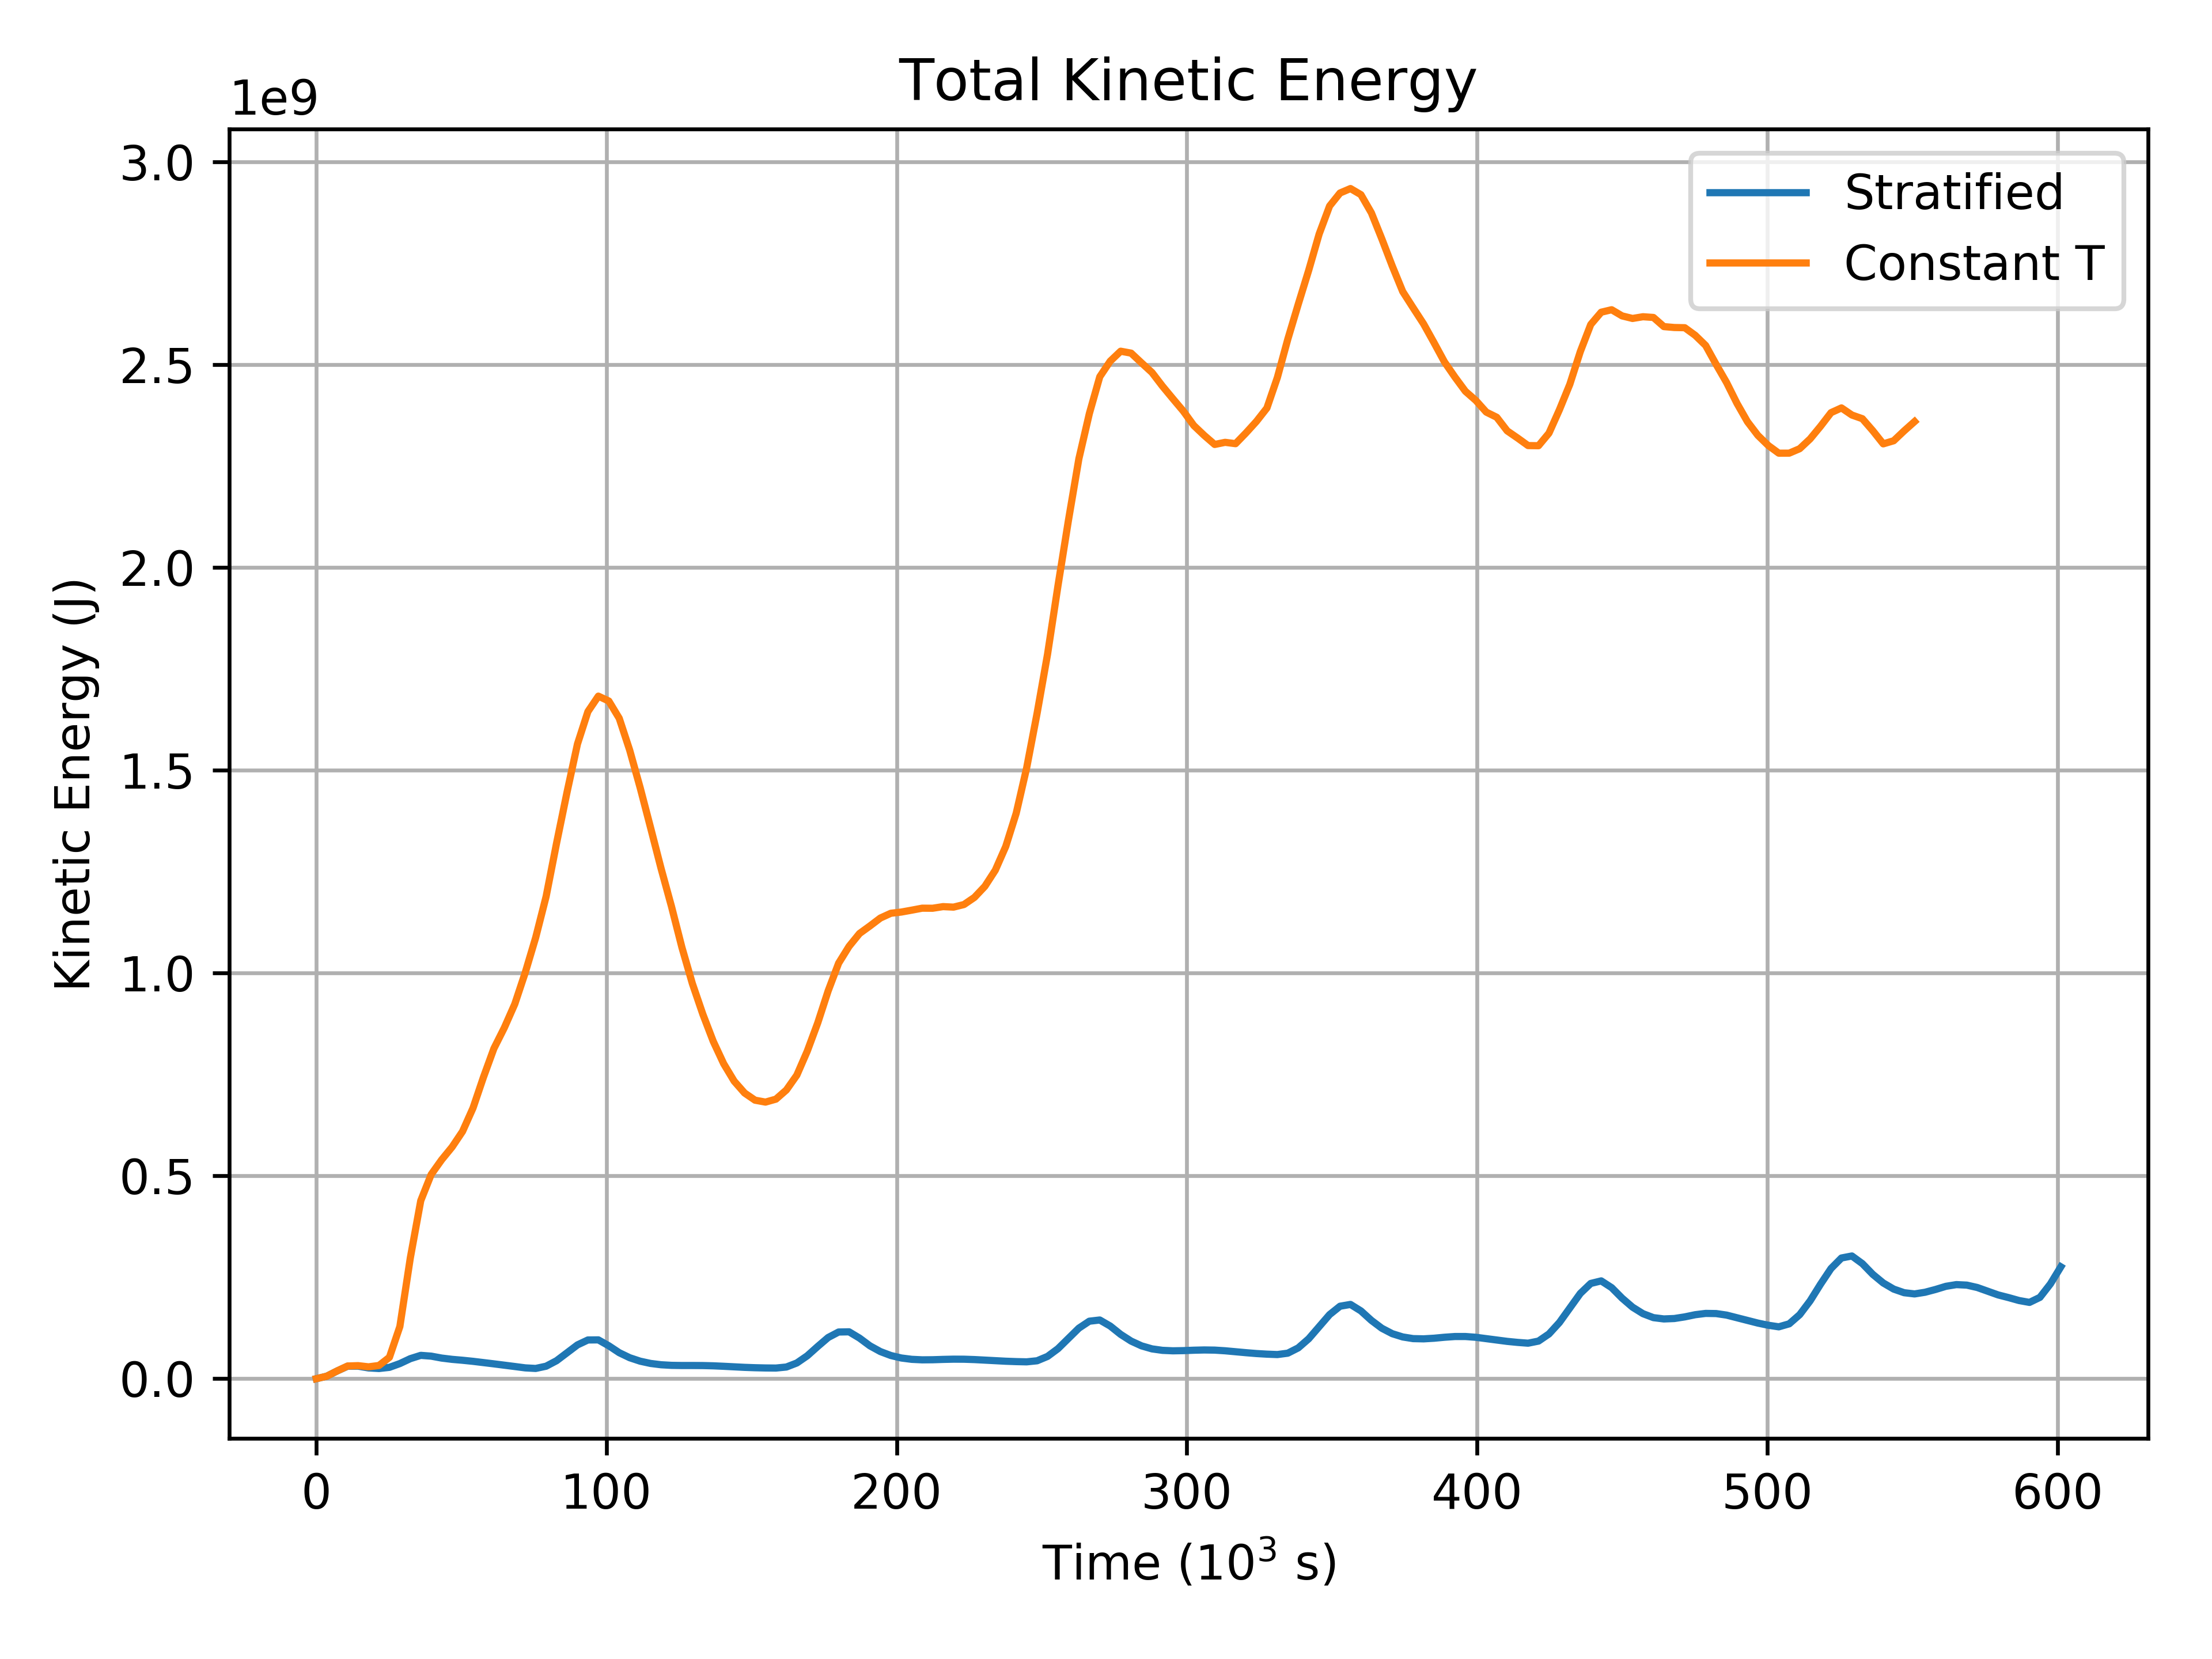
\includegraphics[width=\linewidth]{periodicForcing/forcing-TKE}
\caption{}
\label{fig:periodicForcingTKE}
\end{subfigure}
\begin{subfigure}{0.48\linewidth}
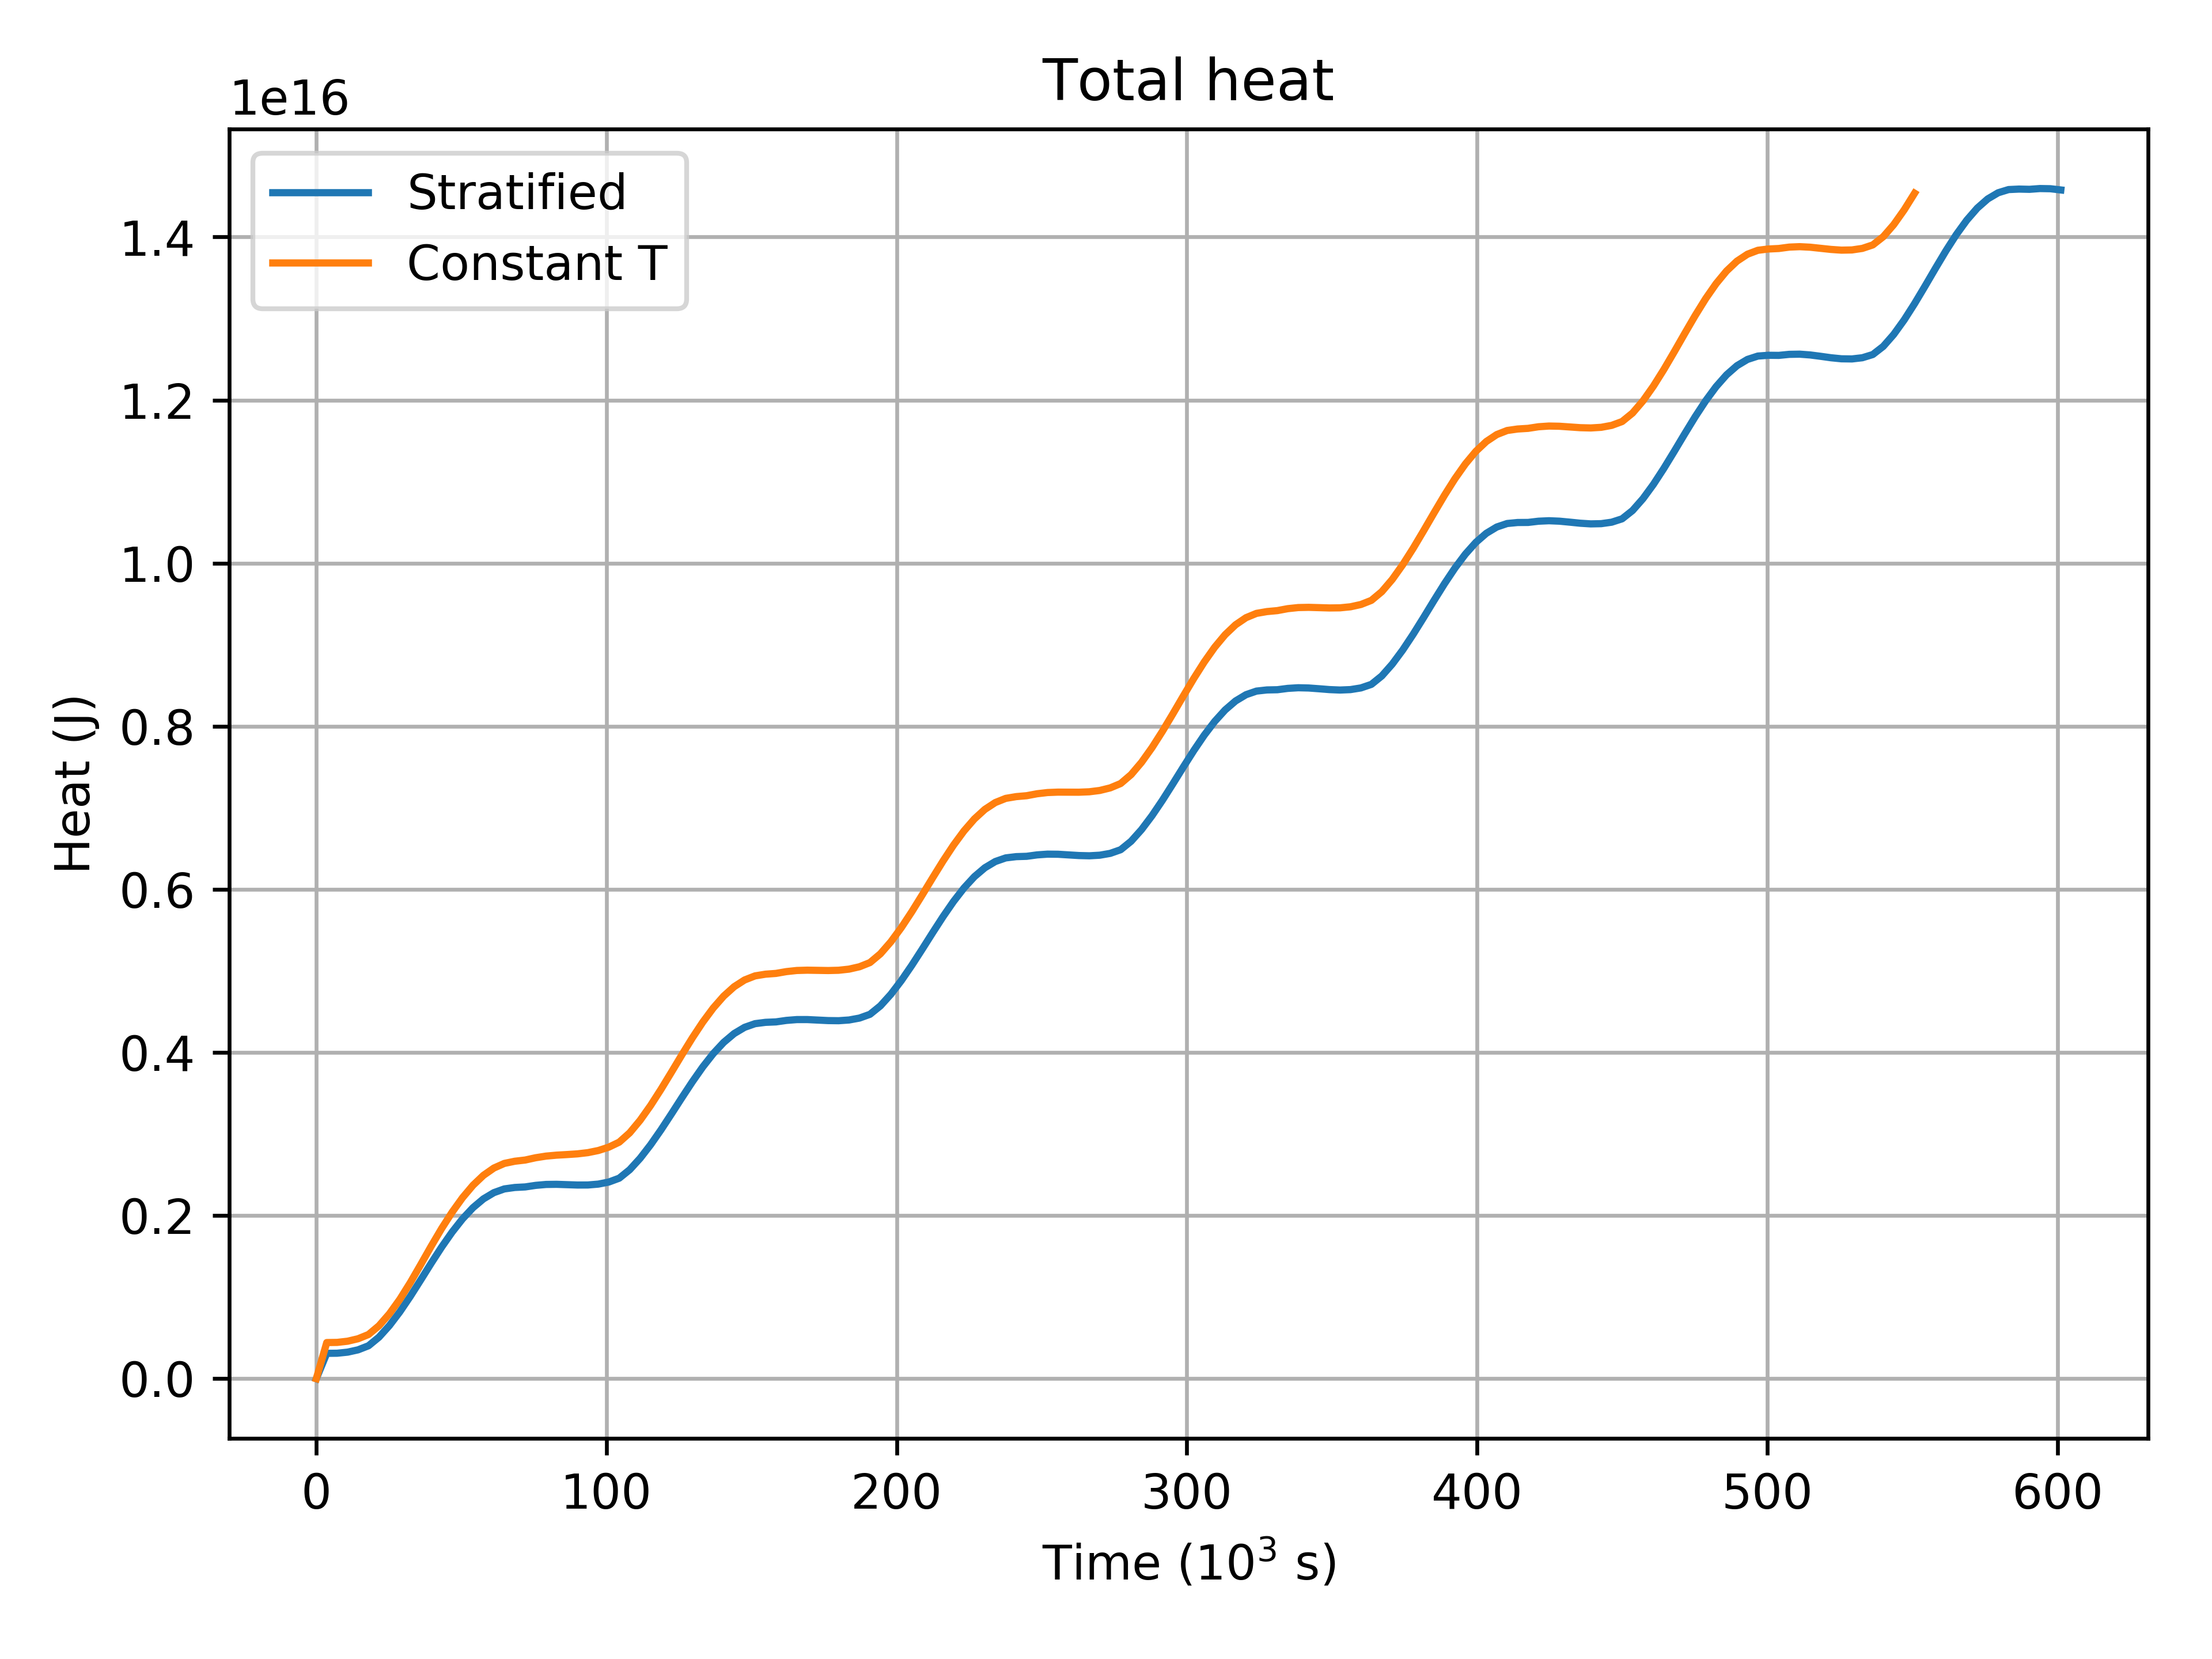
\includegraphics[width=\linewidth]{periodicForcing/forcing-Q}
\caption{}
\label{fig:periodicForcingQ}
\end{subfigure}
\caption{Case 4: comparison of total kinetic energy (top) and internal energy (bottom) between temperature stratified and non-stratified cases.}
\end{figure}

However, the total kinetic energy is significantly higher in the constant temperature case, shown in figure \ref{fig:periodicForcingTKE}. The difference is mostly due to the vertical velocity. When a cold parcel of water near the top of the lake is heated by the sun it warms, and gets denser. This water then starts moving downward. In the stratified case, near the pycnocline there is a restoring buoyant force which should slow or stop the vertical motion. In the non-stratified case, there is no restoring force and the parcel should continue falling and accelerating. I think this is the reason for the significant difference in kinetic energy. However, this should be computed with available/background potential energy.

In the end, the kinetic energy difference might not be very significant. The internal energy (\ref{fig:periodicForcingQ}) is 7 orders of magnitude greater than the kinetic energy by the end of the simulation.

\subsubsection{What we learned}
From running this case, we learned how to include time-dependent forcing with the EXF package (see description of EXF package, section \ref{sec:EXF})

\subsubsection{Next steps}
For this case, there are some clear next steps:
\begin{itemize}
\item{Simulate a more realistic daily cycle in the forcing, and try to bring in real meteorological observations}
\item{Compute the full potential/kinetic/internal energy budget}
\item{Diagnose why the constant temperature case NaN before the stratified case}
\end{itemize}

\subsection{Case 5: 1D comparison}
\label{sec:CLIMo}
Taken together, the results presented above show the model behaves well qualitatively. Now we want to validate the model quantitatively.

One way to quantitatively validate the model is to compare to a simple 1D model which has been validated against observations. A good candiate for this is the Canadian Lake Ice Model (CLIMo) (\cite{Duguay2003}). CLIMo has a simple formulation compared to MITgcm, and is very quick to run (seconds for a year of model time).

\subsubsection{Comparison case}
We design a very simple case to compare the two models. We run MITgcm with a small, shallow square lake (2 km x 2 km x 2 m). We exclude wind forcing, and include constant air temperature, humidity, shortwave and longwave downward radiation. We run a few cases with varying downward radiation values.

CLIMo had to be modified slightly for our purposes: The shortwave and longwave downward radiation were forced to a constant specified value that is a new input into the model instead of computing values from cloud cover and seasonal cycles. To better match MITgcm, CLIMo's ice emissivity is set to be $\varepsilon = \frac{\SI{5.5e-8}{}}{\SI{5.67e-8}{}} \approx 0.98$, which is exactly what MITgcm uses. CLIMo's freezing temperature is set to $\SI{-1.96}{\celsius}$, which is the value of the input \verb|SEAICE_freeze| in MITgcm.

I changed CLIMo to make these changes, which in some sense is backwards. We should ideally be changing MITgcm to agree better with CLIMo since CLIMo is supposed to be the validated model. In practice it is much easier and faster to change parameters in CLIMo and see how it changes the agreement. Then once they agree better, we can revert CLIMo to its validated state and change the corresponding parameters in MITgcm. That being said, some of the changes to CLIMo are trying to explain the disagreement rather than correct it, including the suggestion to reduce CLIMo to have 1 ice layer.

We run both models with four radiation cases:
\begin{enumerate}
\item{$\SI{0}{W.m^{-2}}$ longwave, $\SI{0}{W.m^{-2}}$ shortwave}
\item{$\SI{75}{W.m^{-2}}$ longwave, $\SI{75}{W.m^{-2}}$ shortwave}
\item{$\SI{125}{W.m^{-2}}$ longwave, $\SI{125}{W.m^{-2}}$ shortwave}
\item{$\SI{0}{W.m^{-2}}$ longwave, $\SI{300}{W.m^{-2}}$ shortwave}
\end{enumerate}

\subsubsection{Comparison results}
The mean ice thickness between the models is compared in figure \ref{fig:CLIMoCompare}. The models agree very well with no downward radiation, and the agreement gets systematically worse with increasing radiation. Considering the differences between the model formulations, the agreement is better than expected.

\begin{figure}[h!]
\begin{subfigure}{0.475\linewidth}
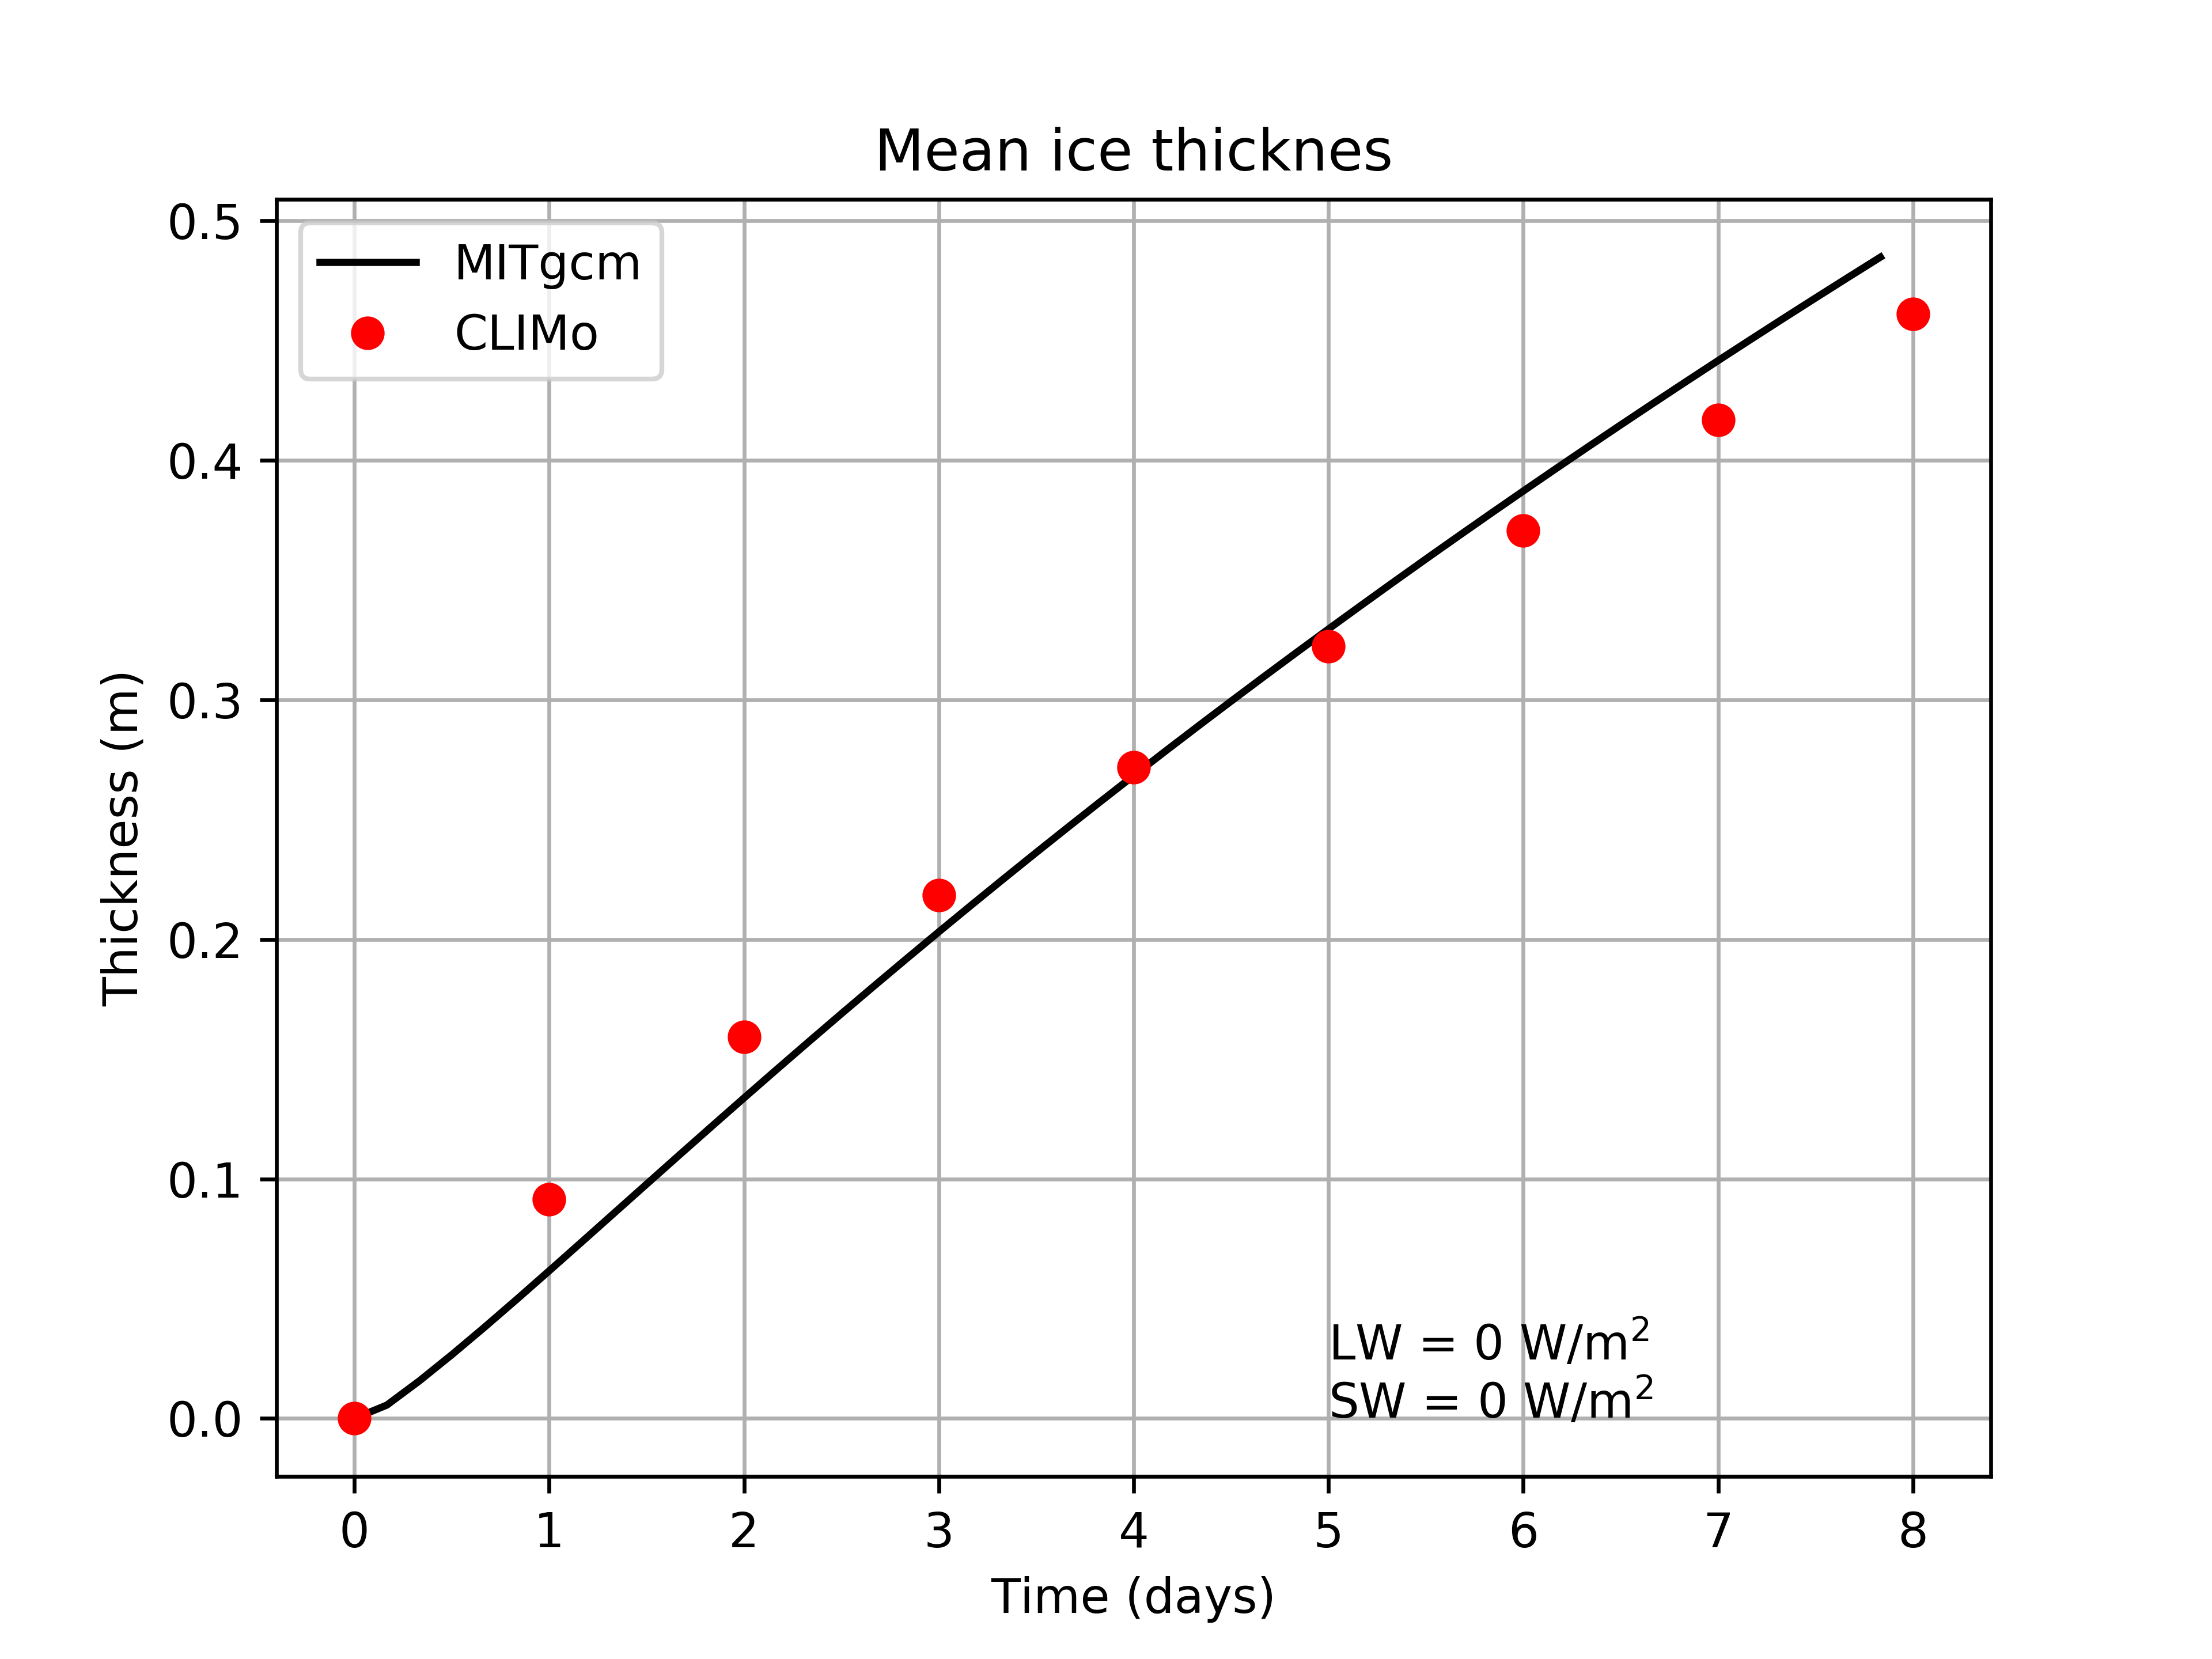
\includegraphics[width=\linewidth]{climo/MITgcm-CLIMo-compare-0-0}
\end{subfigure}
\begin{subfigure}{0.475\linewidth}
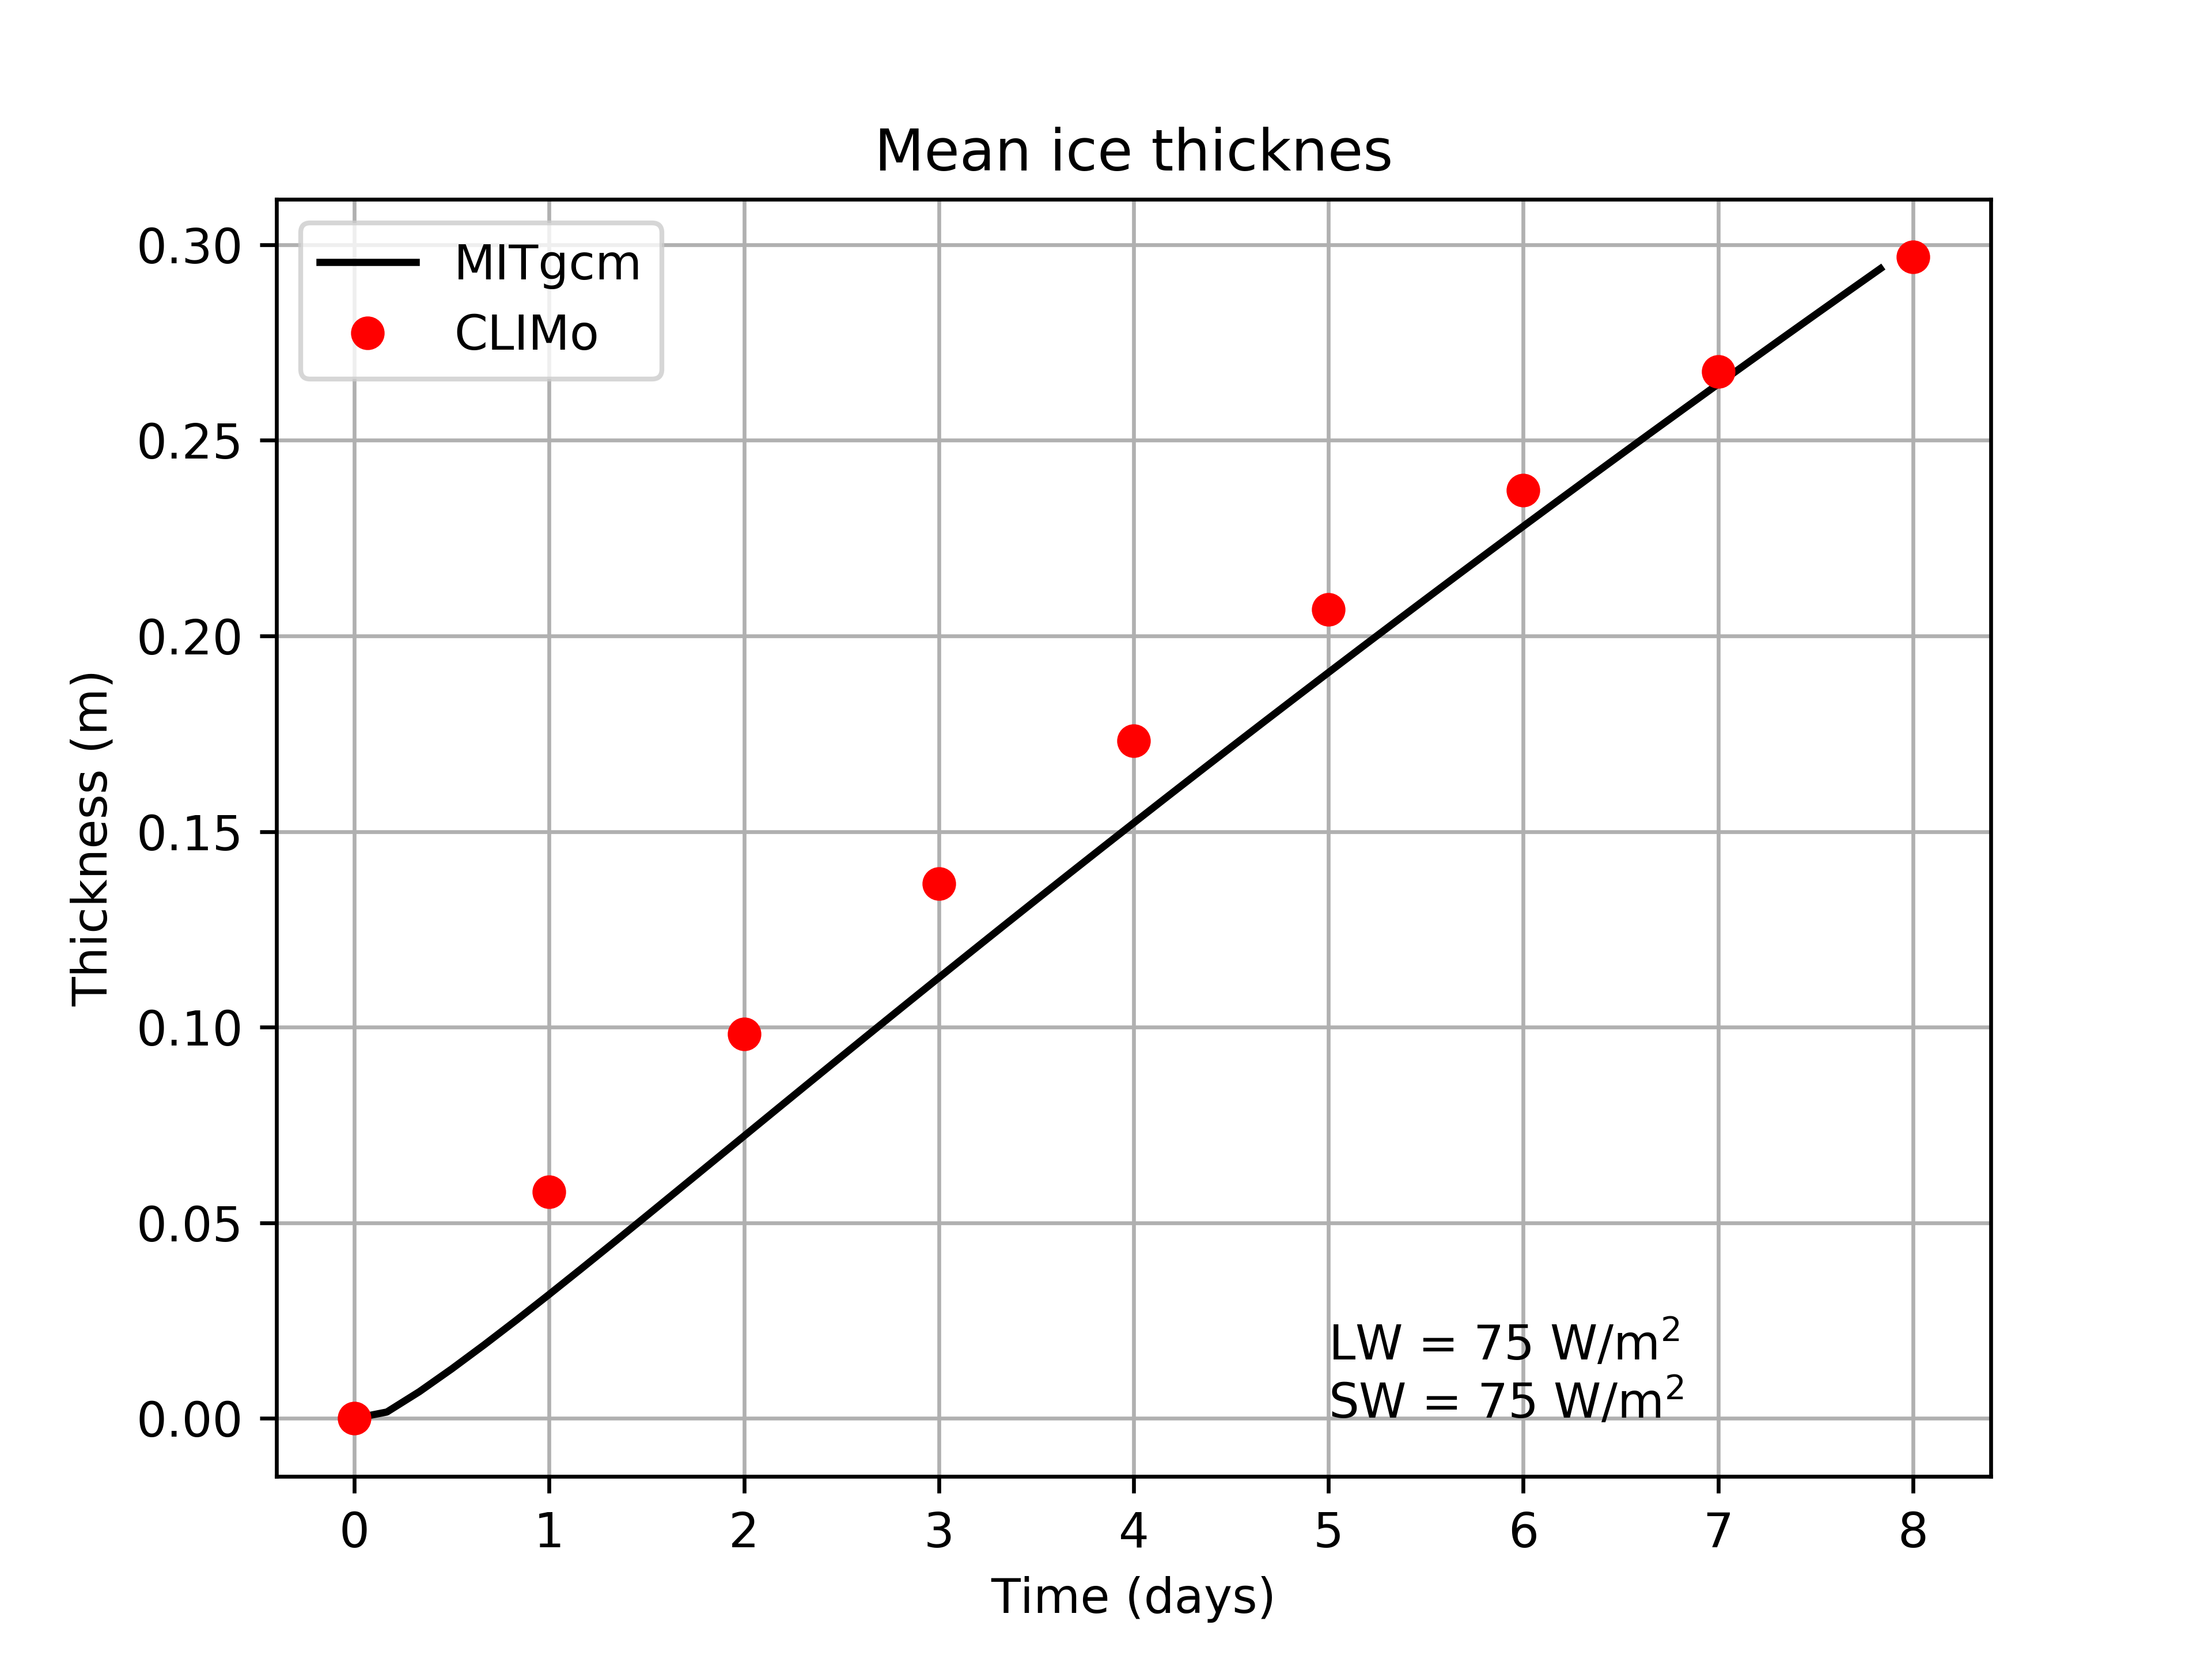
\includegraphics[width=\linewidth]{climo/MITgcm-CLIMo-compare-75-75}
\end{subfigure}

\begin{subfigure}{0.475\linewidth}
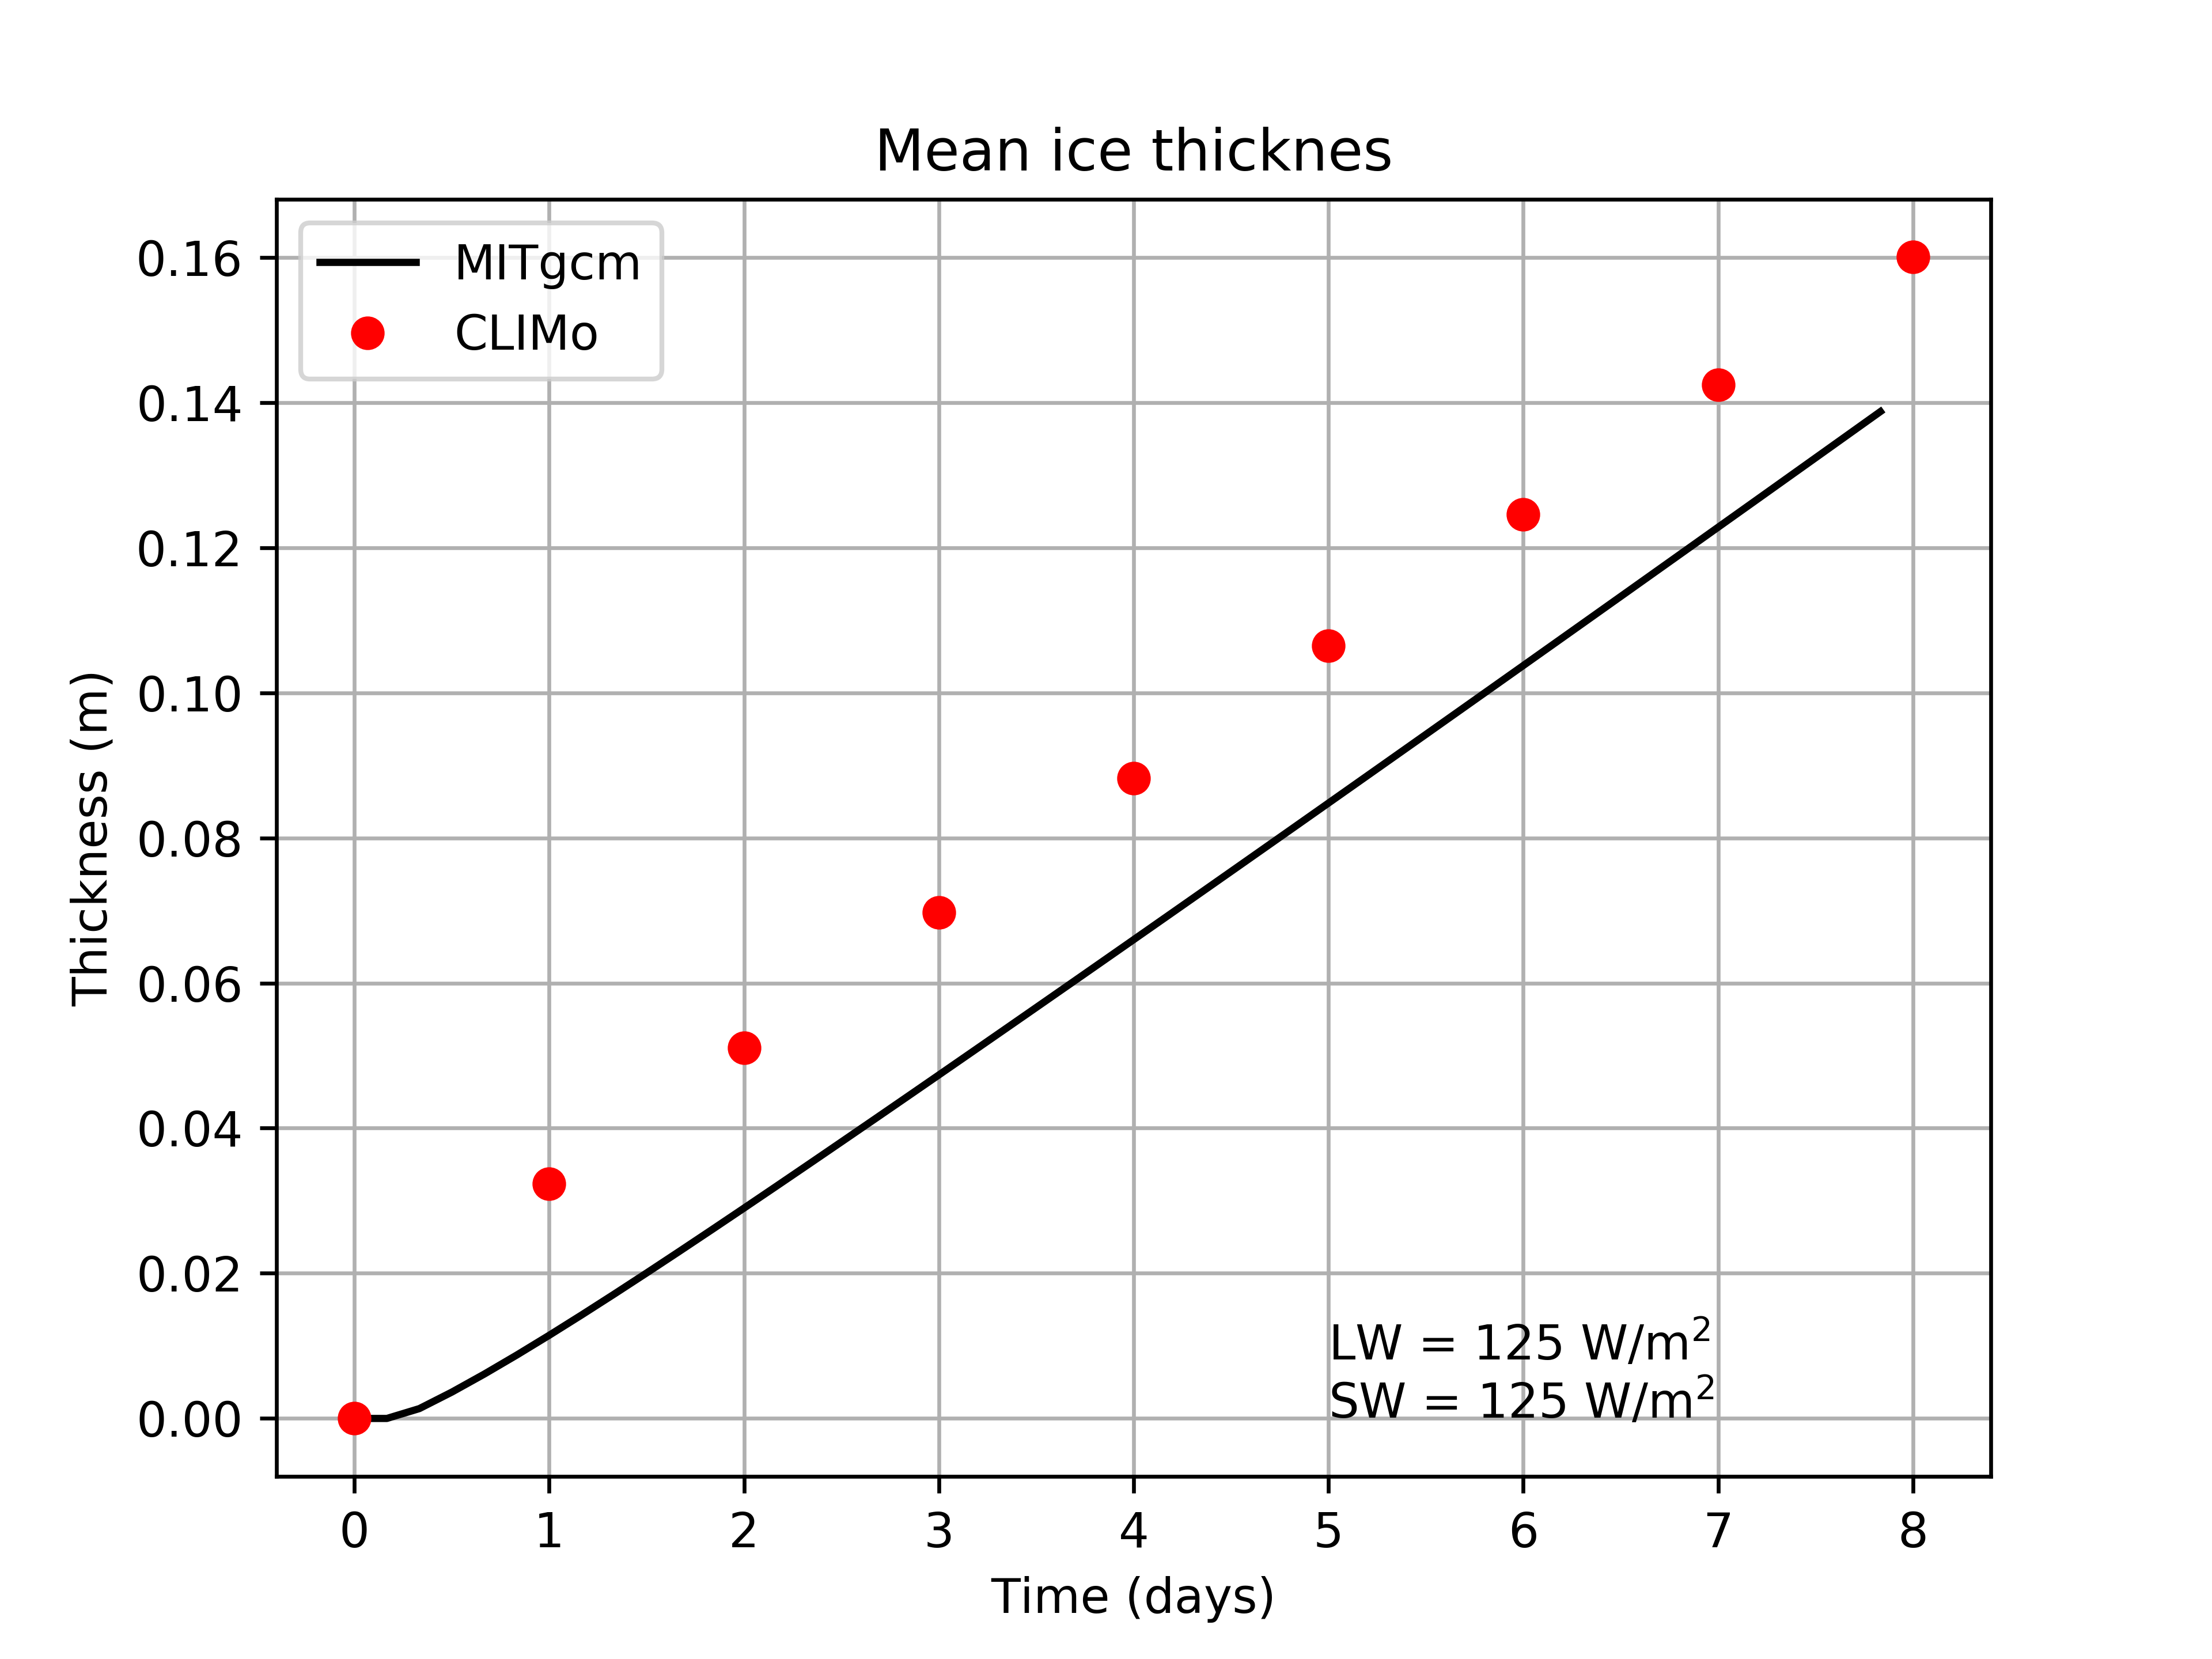
\includegraphics[width=\linewidth]{climo/MITgcm-CLIMo-compare-125-125}
\end{subfigure}
\begin{subfigure}{0.475\linewidth}
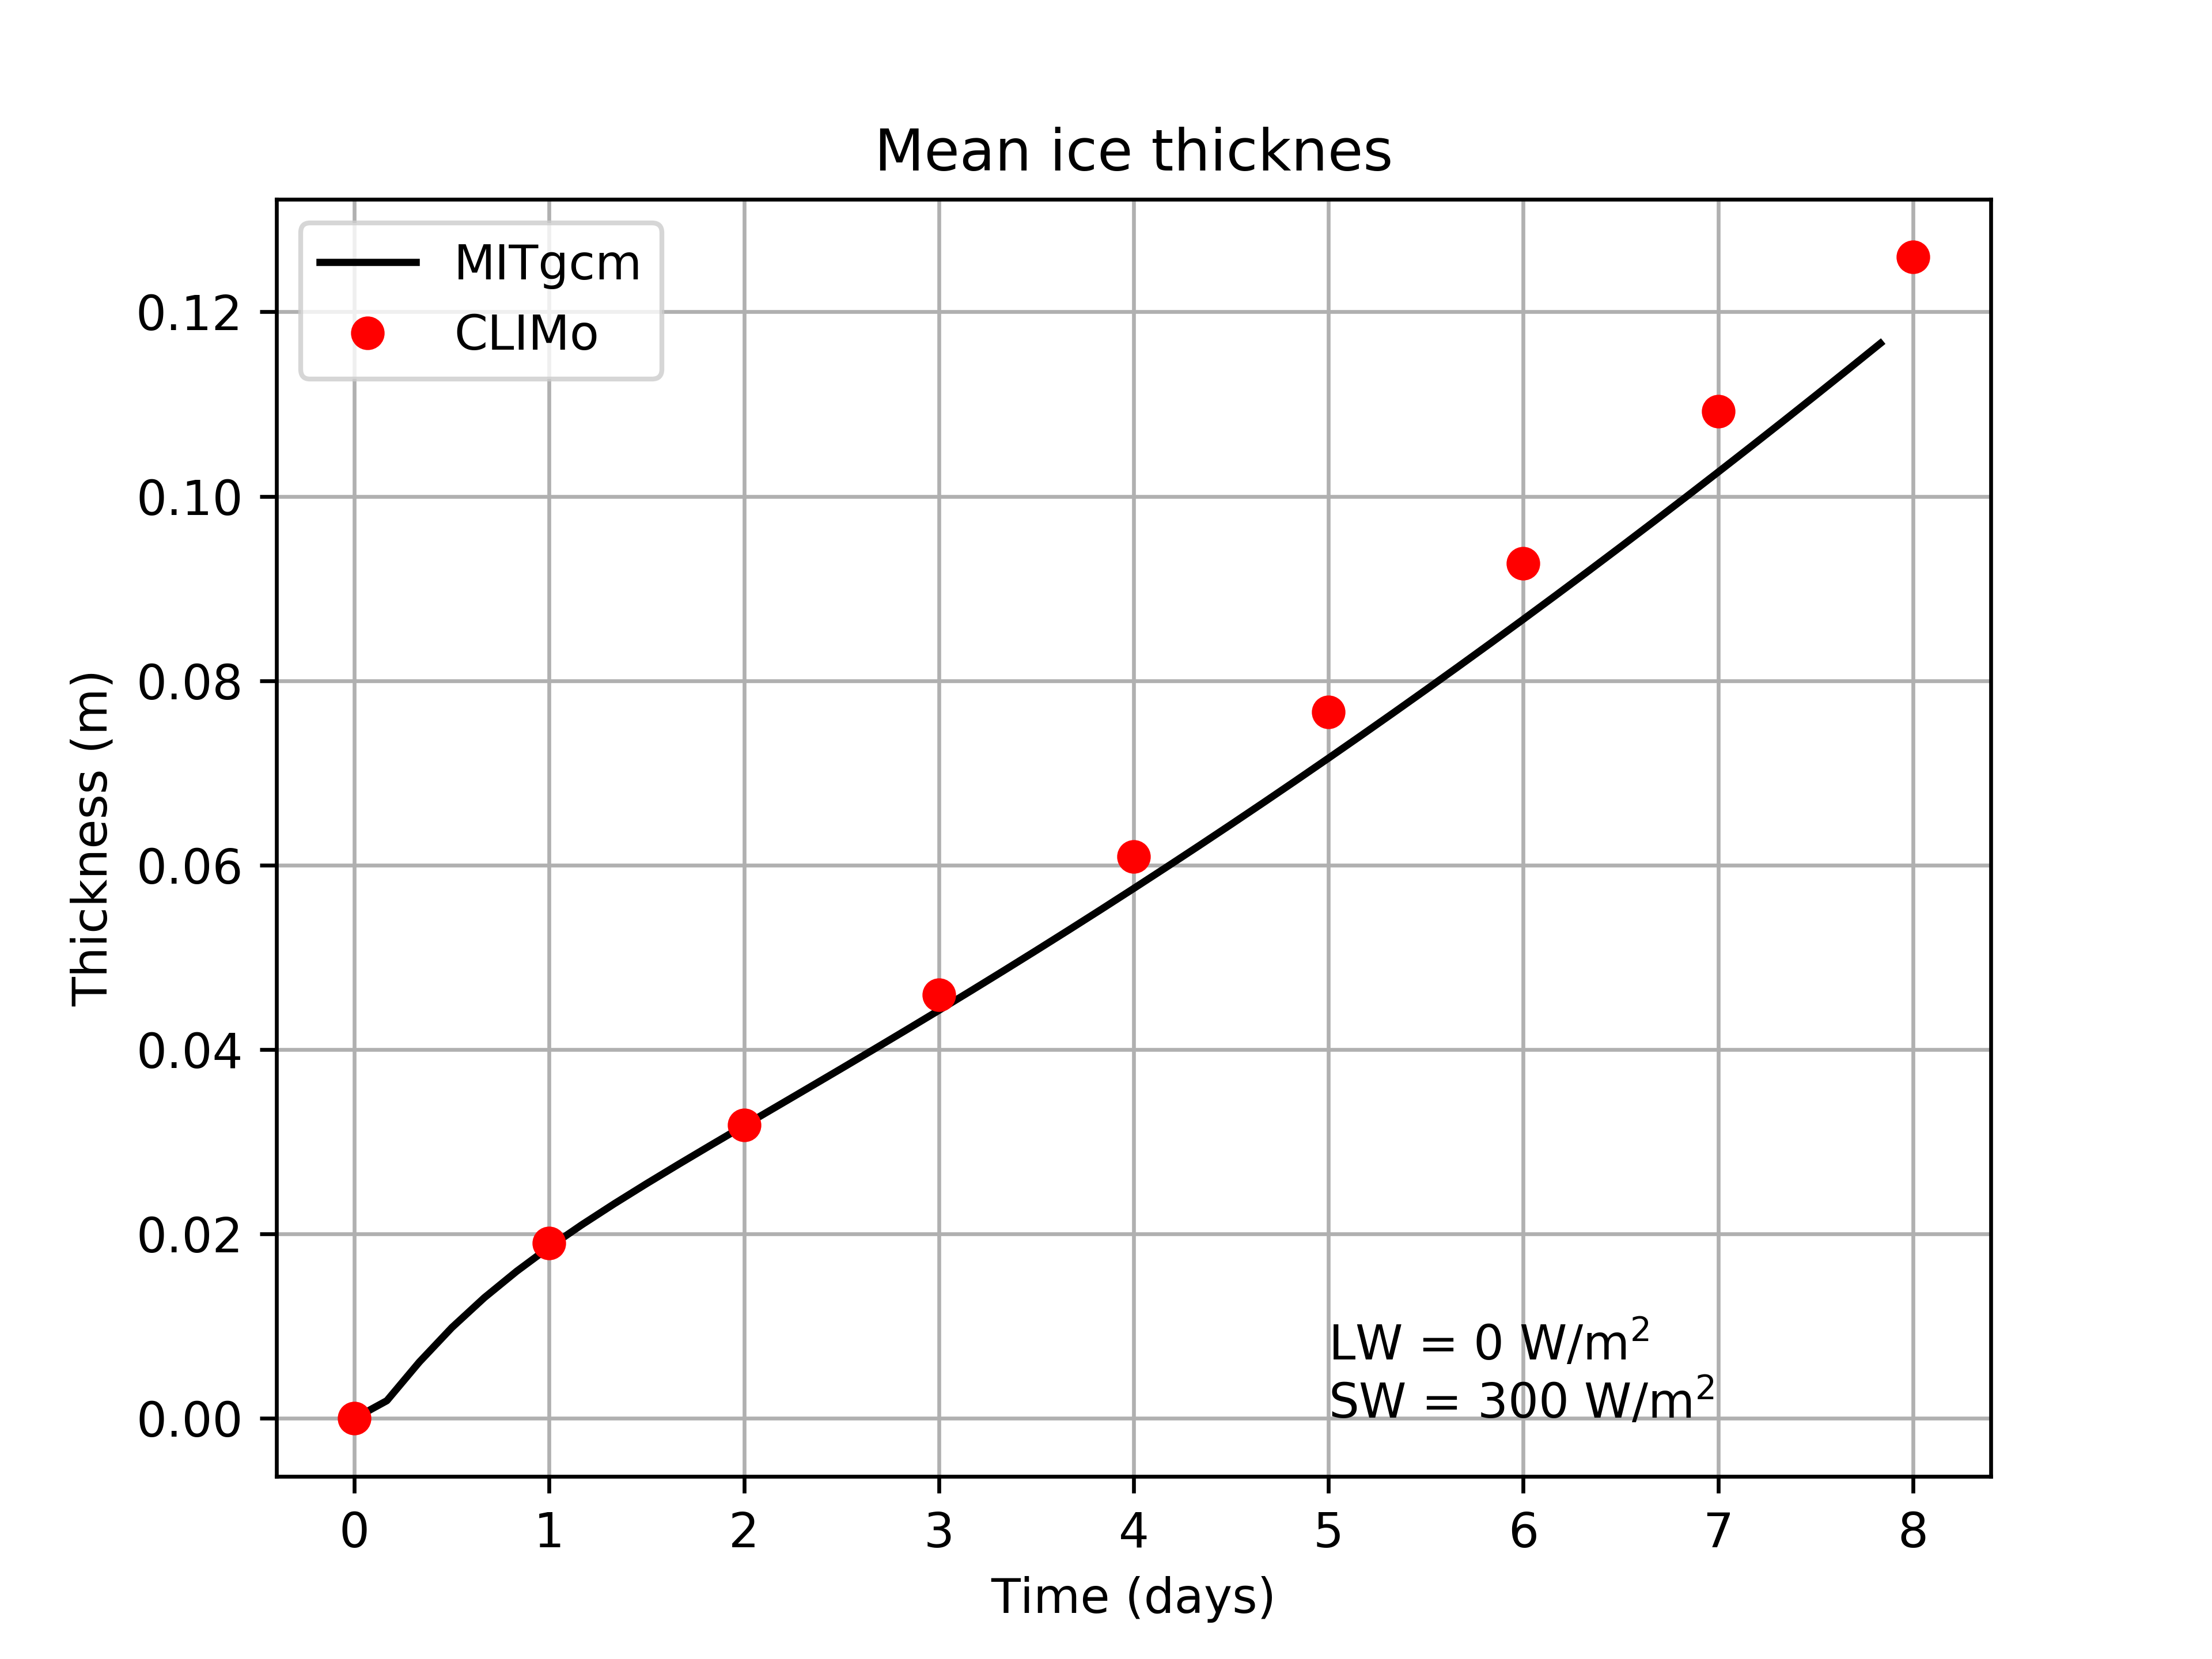
\includegraphics[width=\linewidth]{climo/MITgcm-CLIMo-compare-0-300}
\end{subfigure}
\caption{Mean ice thickness comparison between MITgcm and CLIMo for varying downward radiation values for case 5.}
\label{fig:CLIMoCompare}
\end{figure}

\subsubsection{Next steps}
The agreement from figure \ref{fig:CLIMoCompare} is very good, but we would like to explain why the error systematically increases with increasing radiation. Some more modifications to try are:
\begin{itemize}
\item{Reduce CLIMo to a 1 layer ice model. The current configuration uses 5 layers, and it may agree better with  layer. There is supposed to be radiation and heat conduction between ice layers, which may explain some of the differences.}
\item{Make the albedo values agree better. As discussed in sec \ref{sec:MITgcmAlbedo}, the albedo used in MITgcm is very high. The CLIMo albedo is computed as $\alpha_{CLIMo} = \max(0.44 \left(h\right)^{0.28} + 0.08, \alpha_{water})$, which is lower than the MITgcm albedo until $\SI{4.5}{m}$, and then is greater. Even worse, it is suggested that CLIMo over-estimates snow-free ice albedo (\cite{Svacina2014}). However, if we decrease the MITgcm albedo we would expect that for increasing radiation it would grow ice slower, which would make the agreement worse.}
\item{Turn off CLIMo's snow capabilities entirely by setting the number of snow layers to 0}
\item{Investigate the shortwave radiation extinction scale in CLIMo. The MITgcm parameterization is discussed in section \ref{sec:MITgcmRadiation}. We know MITgcm is hard-coded to a clear ocean water type, maybe if we make the shortwave radiation extinction agree with CLIMo better it will be more applicable to lake modelling.}
\item{For completeness, run a case with downward longwave radiation and no downward shortwave radiation}
\end{itemize}
If the comparison is still interesting, some more long term things to consider:
\begin{itemize}
\item{Compare seasonal ice growth between the models. Run CLIMo and MITgcm with seasonal forcing and compare ice on/off dates and maximum ice thickness.}
\item{Keep CLIMo around, and periodically compare more complicated runs. This might point out areas where either model could be improved}
\end{itemize}


\section{Recurring issues}

\subsection{NetCDF/HDF5 libraries}
I have periodically had problems with the NetCDF/HDF5 libraries. These problems usually came from running out of disk space or disk quotas, but sometimes show up when the wrong modules are loaded. When processing the model binary output files to netCDF files, sometimes the process fails with a generic netCDF or HDF library error. This may be caused by one of the two issues below.

\subsubsection{Disk space or quota}
The first time this issue came up, I had run out of my disk quota on Graham. Try running the bash command \verb|ls -l|. You want to see something like \verb|drwxr-s--- 3 tghill ctb-mmstastn   4096 Jul 24 14:08 include| for each line. Of the two names, the second should be \verb|ctb-mmstastn|, because then your file storage will count towards the contributed resource space, instead of your own (or elsewhere). If a file shows up with group ownership that is your username (or another supervisor who has smaller storage space), you can change the ownership by running \verb|chown [username]:ctb-mmstastn| (or a different group name). If you want to run MITgcm on Hood, ask Robyn for access to a project disk to work on.

\subsubsection{Modules}
The loaded modules on Graham can also present problems. I haven't been able to determine which modules don't work together when running or compiling the model, but to install and use NetCDF tools, the NetCDF and HDF modules should be loaded. You can seach for the current versions with  the command \verb|module spider netcdf|, \verb|module spider hdf5|. If you're compiling and running in parallel, you might need to load the mpi versions. The list of modules below has worked for me for compiling, running, and converting output to netCDF.

\begin{itemize}
\item{StdEnv/2016.4}
\item{nixpkgs/16.09}
\item{imkl/11.3.4.258}
\item{intel/2016.4}
\item{openmpi/2.1.1}
\item{hdf5/1.8.18}
\item{netcdf-mpi/4.1.3}
\end{itemize}

\subsection{MITgcm python utils}
A python \verb|FutureWarning| comes up when running the netCDF conversion package from \verb|gcmpy| with python 3. This might become an Exception in python 3.7. This is caused by a problem in the MITgcmutils package that ships with MITgcm.

The problem line was fixed in commit \href{https://github.com/MITgcm/MITgcm/commit/36b33d0052b0c72fb6cc21138bf556aa3c96c9f1}{36b33d0d}, see \href{https://github.com/MITgcm/MITgcm/pull/140}{this pull request}. Any model code before this change should be updated to the most recent version with this issue fixed.

\section{Physics of the model}
The model uses physical parameterizations that are usually documented to some extent in the MITgcm documentation. As part of getting the model up and running, I looked into some of the parameterizations and compared to what we expect.

\subsection{Radiative cooling}
We looked into the radiative cooling of ice when starting to compare MITgcm ice growth rates to the 1-D model CLIMo (Canadian Lake Ice Model).

The radiative cooling should follow the Stefan-Boltzmann law for total radiative power $M$
\begin{equation}
M = \varepsilon \sigma T^4
\end{equation}
Where $M$ is the radiant emittance (\si{W.m^{-2}}), $\varepsilon$ is the emissivity, and $\sigma = \SI{5.670373e-8}{W.m^{-2}.K^{-4}}$ is the Stefan-Boltzmann constant.

The peak wavelength of the spectral distribution should follow Wien's law
\begin{equation}
\lambda_{max} = \frac{b}{T}
\end{equation}
Where $b = \SI{2.898e-3}{m.K}$ is Wien's displacement constant and T is the temperature. For \SI{0}{\celsius}, $\lambda_{max} \approx \SI{e-5}{m}$ is deep in the infrared (longwave). Therefore, all the radiant emittance should be captured as upward longwave radiation.

The emittance will depend on the value of emissivity used. The SEAICE packages takes in ice emissivity with the variable \verb|SEAICE_emissivity| which is actually $\sigma \varepsilon$. The default value is $\sigma \varepsilon = \SI{5.50e-8}{ W.m^{-2}.K^{-4}}$.  Computing the expected emittance, 

\begin{equation*}
M = \SI{306.17}{W.m^{-2}}
\end{equation*}

The model shows very good agreement with this value.	

\subsection{Water surface energy budget}
As one way to compare the effect of parameters and meteorological forcing values, we compute the total internal energy in heat of the water, as well as the heat fluxes across the water boundary. We expect that

\begin{equation}
\frac{d Q}{d t} = \Phi_{net} = \Phi_{ice} + \Phi_{atm}
\end{equation}

The model outputs $-\Phi_{net}$ as the diagnostic \verb|SIqnet| (heat flux from the water into ice if ice covered, atmosphere if open water). To check this, we compute the internal energy of the water as

\begin{equation}
Q = c_w \sum_{x, y, z} \rho \Delta V \Delta T
\end{equation}
Where the sum is over all grid cells, $\Delta V$ is the volume of each cell, and $\Delta T$ is the temperature at time $t$ minus the initial temperature.

The derivative is taken using the most basic scheme,

\begin{equation*}
\frac{d Q}{d t} \approx \frac{Q(t_{n+1}) - Q(t_n)}{t_{n+1} - t_n}
\end{equation*}

Finally, a plot of $\frac{d Q}{d t} + \verb|SIqnet|$ should be near zero (not identically zero because of the derivative scheme) for all times. We have found this to be the case.

\subsection{Surface albedo}
\label{sec:MITgcmAlbedo}
In comparing the MITgcm ice growth rate to CLIMo, I investigated the albedo parameterization of MITgcm. The model classifies ice according to the temperature of the surface water $T_{surf}$ comapred to the freezing/melting temperature $T_{melt}$

\begin{equation*}
\textrm{ice} = \begin{cases} \textrm{dry}, & T_{surf} < T_{melt} \\ \textrm{wet}, & T_{surf} \geq T_{melt} \end{cases}
\end{equation*}
The default ice albedo is
\begin{equation*}
\alpha_i = \begin{cases} 0.75, T_{surf} < T_{melt} \\ 0.66, T_{surf} \geq T_{melt} \end{cases}
\end{equation*}
The default snow albedo is
\begin{equation*}
\alpha_s = \begin{cases} 0.84, T_{surf} < T_{melt} \\ 0.70, T_{surf} \geq T_{melt} \end{cases}
\end{equation*}
And the values are controlled by the input variables \verb|SEAICE_dryIceAlb|, \verb|SEAICE_wetIceAlb|, \verb|SEAICE_drySnowAlb|, and \verb|SEAICE_wetSnowAlb|.

\subsection{Thermodynamics}
The SEAICE package is mainly intended for ice dynamics, but includes basic thermodynamics. The THSICE package is be fully compatible with SEAICE and include improved thermodynamics. However, the THSICE package is not well suited for freshwater simulations, so for the purpose of this document it is recommended to continue to use only the SEAICE package for dynamics and thermodynamics.

The THSICE package is intended to improve the thermodynamics of saltwater ice. When ice forms over salt water, some pockets of salt water called brine pockets get trapped in the ice. These brine pockets provide interesting thermodynamics. When the ice is warmed, some of the ice around the brine pockets will be melted. This meltwater must be freshwater, so it dilutes the salt in the brine pocket. This can sufficiently dilute the brine pocket so that the pocket freezes completely, releasing latent heat to the surrounding ice \cite{Winton2000}.

Clearly this process is irrelevant for freshwater lake ice. While the three-layer formulation of \cite{Winton2000} is an improvement over what is described in the \href{http://mitgcm.org/public/r2_manual/final/online_documents/node254.html}{SEAICE documentation}, the implementation does not work for freshwater. The model tends to NaN once ice starts to form. Moreover, the SEAICE documentation says ``NOTE: THIS SECTION IS TERRIBLY OUT OF DATE'' about the thermodynamics description in the documentation. Therefore, we can't really compare the packages anyways.

On a more practical note, the THSICE package breaks the model with any good advection schemes. It runs (with unphysical results, no ice motion) advection scheme 2. With 33 or 77 (77 is highly recommended for this package) it breaks the model very quickly, often after the first time step. We have enough justification to exclude the package from our simulations.

\subsection{Total kinetic energy}
I compute the total kinetic energy of the water as an additional way to compare the differences between different parameters and configurations. The total kinetic energy is computed as
\begin{equation}
\textrm{TKE} = \frac{1}{2} \sum_{x, y, z} \rho \left ( u^2 + v^2 + w^2\right ) \Delta V
\end{equation}
Where $\rho = \rho_0 + \rho^{\prime}$ is the total (reference + anomaly) density of the gri cell, $u, v, w$ are the $x, y, z$ velocities, and $\Delta V$ is the volume of the grid cell.

\subsection{Dynamical ice model}
\label{sec:iceDynamics}
The equation governing the dynamical evolution of the ice is the conservation of momentum equation

\begin{equation}
m \frac{D \mathbf{u}}{D t} = -m f \mathbf{k}\times \mathbf{u} - m\nabla \phi(0) + \mathbf{F} + \mathbf{\tau_{air}} + \mathbf{\tau_{ocean}}
\end{equation}

Where  $m = m_i + m_s$ is the total mass of ice and snow per unit area, $\phi(0)$ is the sea surface height potential, $\mathbf{F} = \nabla \cdot \sigma$ is the divergence of the ice stress tensor, and $\tau_{air}, \tau_{ocean}$ are the wind-ice and ocean-ice stresses. The wind and ocean stresses are parameterized as

\begin{equation}
\begin{aligned}
\mathbf{\tau_{air}} &= \rho_{air}C_{air}\left \| \mathbf{U}_{air} - \mathbf{u} \right \| R_{air}\left(\mathbf{U}_{air} - \mathbf{u}\right) \\
\mathbf{\tau_{water}} &= \rho_{water}C_{water}\left \| \mathbf{U}_{water} - \mathbf{u} \right \| R_{water}\left(\mathbf{U}_{water} - \mathbf{u}\right)
\end{aligned}
\end{equation}

Where $\mathbf{U_i}$ are the surface winds of the atmosphere and water, $C_i$ are air and water drag coefficients, $\rho_i$ are reference densities, and $R_i$ are rotation matrices.

\subsection{Radiation}
\label{sec:MITgcmRadiation}
The model can be forced with net or downward shortwave and longwave radiation. Longwave radiation is absorbed by the surface layer, while shortwave radiation penetrates into the interior of the water. This section describes the penetrating shortwave radiation. The equations here come from \cite{PaulsonSimpson1977} and the source code, particularly \verb|pkg/exf/exf_radiation.F|, \verb|model/src/swfrac.F| and \verb|model/src/external_forcing.F|.

First, consider the amount of shortwave radiation that is transmitted through the surface. The reflected shortwave radiation is the product of the surface albedo and the incoming shortwave radiation, $\alpha I_{down}$. Then, the amount absorbed into the water is

\begin{equation}
I_0 = (1 - \alpha) I_{down}
\end{equation}

The radiation transmission model \cite{PaulsonSimpson1977} splits the radiation into two wavelength bands. Each decays exponentially

\begin{equation}
\frac{I}{I_0} = R e^{-z/\zeta_1} + (1 - R) e^{-z/\zeta_2}
\end{equation}
Where $I$ is the radiation at depth $z$ (positive from the surface), and $R = 0.62$, $\zeta_1 = \SI{0.60}{m}$, $\zeta_2 = \SI{20}{m}$ are constants that come from Jerlov water type IA. This water type represents clear ocean water, and is hard-coded into MITgcm.

This treatment should work well for relatively deep water, but for shallow lakes this is a problem. For example, with a 2 m deep lake approximately 37\% of the radiation makes it to the bottom of the lake. This radiation should then be absorbed by the bottom and eventually heat the lake from the bottom, but this is not accounted for.

\subsection{Humidity}
The EXF package uses specific humidity (input as \verb|aqhfile|), which is the ratio of the mass of water vapour to the total mass of a unit volume of air. This is different than relative humidity, which we are generally more familiar with.

The comparison between relative humidity and specific humidity depends on temperature and atmospheric pressure. The conversion is outlined below. Constants are given in table \ref{table:humidityConstants}

\begin{table}
\begin{tabularx}{\textwidth}{X X X}
\hline
\textbf{Symbol} & \textbf{Name} & \textbf{Value} \\ \hline \hline
$N$ & Avogadro's number & $\SI{6.022e23}{{mol}^{-1}}$ \\ \hline
$R$ & Ideal gas constant & $\SI{8.3145}{J.{mol}^{-1}}$ \\ \hline
$M_{H2O}$ & Molar mass of water & $\SI{18.01534}{g.{mol}^{-1}}$ \\ \hline
$M_{dry}$ & Molar mass of dry air & $\SI{28.9644}{g.{mol}^{-1}}$ \\ \hline
\end{tabularx}
\caption{Constants for relative humidity calculation}
\label{table:humidityConstants}
\end{table}

The most relevant direction is to compute specific humidity from relative humidity. We would usually choose a relative humidity value, and want to find the corresponding specific humidity to input to the model. The specific humidity is the mass ratio of water vapor to dry air. That is,

\begin{equation}
\label{eq:specificHumidity}
q = \frac{X_{H2O}M_{H2O}}{X_{H2O}M_{H2O} + \left(1 - X_{H2O}\right) M_{dry}}
\end{equation}
Where $X_{H20}$ is the molar mixing ratio (equivalent to pressure ratio), 
\begin{equation}
X_{H2O} = \frac{P_{H2O}}{P}
\end{equation}
$P_{H2O}$ is the partial pressure of water vapour, and $P$ is the atmospheric pressure (in Pa). The partial pressure of water is given by
\begin{equation}
P_{H2O} = \frac{R \cdot e(T)}{100}
\end{equation}
Where $R$ is the relative humidity (\%), $T$ is the temperature ($^{\circ}\textrm{C}$) and $e(T)$ is the vapour pressure of water (Pa),
\begin{equation}
e = 100 \left[a_0 + T \left( a_1 + T \left( a_2 + T \left( a_3 + T \left( a_4 + T \left( a_5 + T a_6 \right) \right) \right) \right) \right) \right]
\label{eq:vapourPressure}
\end{equation}
The constants are given for water and ice in table \ref{table:vapourConstants}, and $e = \min\left({e_{water}},{e_{ice}}\right)$.

\begin{table}
\begin{tabularx}{\textwidth}{c c c}
\hline
\textbf{NA} & \textbf{Water} & \textbf{Ice} \\ \hline \hline
$a_0$ & \SI{6.107799961}{} & \SI{6.109177956}{} \\ \hline
$a_1$ & \SI{4.436518521e-1}{} & \SI{5.034698970e-1}{} \\ \hline
$a_2$ & \SI{1.428945805e-2}{} & \SI{1.886013408e-2}{} \\ \hline
$a_3$ & \SI{2.650648471e-4}{} & \SI{4.176223716e-4}{} \\ \hline
$a_4$ & \SI{3.031240396e-6}{} & \SI{5.824720280e-6}{} \\ \hline
$a_5$ & \SI{2.034080748e-8}{} & \SI{4.838803174e-8}{} \\ \hline
$a_6$ & \SI{6.136820929e-11}{}& \SI{1.838826904e-10}{}\\ \hline
\end{tabularx}
\caption{Vapour pressure constants for equation \ref{eq:vapourPressure}}
\label{table:vapourConstants}
\end{table}

All together with $e(T)$ given by \ref{eq:vapourPressure},

\begin{equation}
\label{eq:humidityConversion}
q = \frac{1}{1 + \frac{P\cdot 100}{R\cdot e(T)} \cdot \frac{M_{dry}}{M_{H2O}}}
\end{equation}

Going the other way, we see that with $q = 0.01$, $T = \SI{-10}{\celsius}$ and $P = 101325 Pa$, the relative humidity is above 500\%. Clearly this is a problem!

The model was run in the configuration from fig \ref{fig:CLIMoCompare} with $\SI{125}{W.m^{-2}}$ downward SW and LW radiation with the original humidity value ($q = 0.01$, $R \approx 580\%$) and a more realistic value ($q = \SI{8.e-4}{}$, $R = 50\%$). The output is exactly identical. Changing the humidity values has no effect on any of the output fields. This is suspicious - humidity should have some effect. This is probably worthwhile to investigate: when does humidity matter? It should matter to evaporation at least. Maybe this case just has no evaporation.

\section{Visualization tools}
Visualization tools for animations of top-down views and cross-sections were developed in python. These are good to get an idea of what is happening in a case, and to compare cases. Code and documentation for these post-processing tools live on \href{https://github.com/timghill/gcmpy}{GitHub here}.

Some basic scripts for 3D visualization in VisIt were also developed. These are more involved to use and develop, but produce much more interesting graphics. These will be added to the wiki as examples of VisIt scripts.

\section{Conclusions}
The cases presented in Results are good toy cases to validate the qualitative dynamics of the MITgcm ice model in freshwater lakes. The model clearly freezes water into ice and melts ice at physical temperatures (with the right advection scheme). The ice dynamics once it forms are intuitively correct. The ice is advected by wind forcing and surface currents, and the ice exerts surface stress on the water in response ($-\tau_{water}$ is applied to the surface layer of water).

The various packages necessary for modelling freshwater lake ice have been used and documented here, and some of the physical parameterizations are examined here. It is determined that the THSICE package that is recommended to be used by the MITgcm documentation is not applicable to freshwater ice. The interesting thermodynamics it is meant to recreate do not exist in freshwater ice, and some detail of the implementation of the package does not work with freshwater.

The comparison to CLIMo is very promising, but has some more work to be done before the model is well validated.

\section{Next steps}
There are some clear directions to extend the cases from Results in that are dicussed within the individual sections. There are some overall directions to go from here:
\begin{itemize}
\item{Make the comparison to the 1D model more complete (sec \ref{sec:CLIMo}}
\item{Include the recommendations from the SEAICE section \ref{sec:SEAICE} into the toy cases}
\item{Learn what the thermodynamic formulation of the SEAICE package is. It might be an interesting project to write a better thermodynamics package for freshwater ice. It could be based on the layer structure of the THSICE package, but with salinity eliminated from the equations}
\end{itemize}

\subsection{What to expect when changing the model}
There is lots to change in the model, and many more runs to carry out. This section gives a rough outline of how long you should expect changing the model to take, and how long some runs will take.

\subsubsection{How long to change the model configurations}

\subsubsection*{Minor changes}
A minor change is something like changing the resolution of the model, change a few run time parameters, or running with different forcing files. These changes don't require recompiling the model, and should only take a few hours at most. It should be easy to estimate how long these changes should take. You shouldn't run in to too many surprise errors.

\subsubsection*{Moderate change}
A moderate change is something like changing the grid size of the model, or changing compile time options of a package. These require recompiling the model and changing run time options. Accounting for some mistakes and compile time, changes like this will probably take a few hours to a day to get running.

\subsubsection*{Significant change}
A significant change is something like adding a new package to the model that you haven't used before, or designing an entire new case from scratch: writing scripts to make the forcing files, setting model parameters, compiling, and fixing all typos and mistakes. This will likely take a few days to flush out all the bugs and weird problems that come out.

\subsubsection{How long to run the model}
The time the model needs to run for is highly dependent on how many processors you run it with. But some general guidelines are below.

\begin{table}
\begin{tabularx}{\textwidth}{X X X X}
\hline
\textbf{Case size} & \textbf{Example} & \textbf{Time expected} & \textbf{Approximate number of processors} \\ \hline \hline
Small & Case 1 and 5 & About 1 to a few hours & 4 - 16 \\ \hline
Medium & Case 3 and 4 & 2 - 12 hours & 16 - 32 \\ \hline
Large & Case 3 hydrodynamic and case 2 hydrostatic & 12 hours to a few days & 25 - 144 \\ \hline
Significant & Case 2 hydrodynamic & Few days to a week & $\mathcal{O}(400)$ \\ \hline
\end{tabularx}
\caption{Approximate case size and run time guidelines}
\label{table:runTime}
\end{table}

A very small case like case 1 or case 5 should take somewhere around an hour to run on a handful of processors (on the order of 8 or 16).

\bibliography{refs}

\end{document}